%%%%%%%%%%%%%%%%%%%%%%%%%%%%%%%%%%%%%%%%%
% Beamer Presentation
% LaTeX Template
% Version 1.0 (10/11/12)
%
% This template has been downloaded from:
% http://www.LaTeXTemplates.com
%
% License:
% CC BY-NC-SA 3.0 (http://creativecommons.org/licenses/by-nc-sa/3.0/)
%
%%%%%%%%%%%%%%%%%%%%%%%%%%%%%%%%%%%%%%%%%

%----------------------------------------------------------------------------------------
%	PACKAGES AND THEMES
%----------------------------------------------------------------------------------------

\documentclass[10pt, a4paper, twoside]{article}
\usepackage{graphicx} % Allows including images
\graphicspath{{../figures/}}
\usepackage{booktabs} % Allows the use of \toprule, \midrule and \bottomrule in tables
\usepackage{amsmath, amssymb, amsthm, gensymb}
\usepackage{mathtools}
\usepackage{hyperref}
\usepackage{epigraph}
\usepackage{etoolbox}
\usepackage{listings}
\usepackage{exercise}
\usepackage{multirow}
\usepackage{array}
\newcolumntype{C}{@{}c@{}}
\newcommand{\bottombox}[1]{\makebox[2em][r]{#1}\hspace*{\tabcolsep}\hspace*{2em}}%
\newcommand{\innerbox}[2]{%
    \begin{tabular}[b]{c|c}
       \rule{2em}{0pt}\rule[-2ex]{0pt}{5ex} & \makebox[2em]{#2} \\\cline{2-2}
       \multicolumn{2}{r}{{#1}\hspace*{1.5\tabcolsep}\hspace*{2em}\rule[-2ex]{0pt}{5ex}}
    \end{tabular}}
\renewcommand{\arraystretch}{1.25}
\makeatletter
\patchcmd{\epigraph}{\@epitext{#1}}{\itshape\@epitext{#1}}{}{}

\usepackage{tikz}
\usetikzlibrary{shapes,arrows,positioning}
\usetikzlibrary{arrows.meta}
\usetikzlibrary{chains,fit,shapes,calc}
\usepackage{adjustbox}
\usepackage{physics}

\newcommand{\uvec}[1]{\textbf{#1}}

\newtheorem{exe}{Exercise}
\newtheorem{program}{Programming exercise}
\newtheorem{theorem}{Theorem}

\usepackage{exercise}

\DeclareMathOperator{\Hessian}{Hess}

\definecolor{myblue}{RGB}{80,80,160}
\definecolor{mygreen}{RGB}{80,160,80}

\newcommand{\colvec}[1]{\begin{pmatrix} #1 \end{pmatrix}}


% extracted from linalgjh.sty from https://github.com/indraniel/linear-algebra

%-------------making aligned columns
% Usage: \begin{aligncolondecimal}{2} 1.2 \\ .33 \end{aligncolondecimal}
% (negative argument centers decimal pt in column).  Also Usage:
% \begin{aligncolondecimal}[0em]{2} 1.2 \\ .33 \end{aligncolondecimal}
% to make the left and right LaTeX-array padding disappear.
\RequirePackage{array}\RequirePackage{dcolumn}
\newenvironment{aligncolondecimal}[2][.1111em]{%
\setlength{\arraycolsep}{#1}
\newcolumntype{.}{D{.}{.}{#2}}\begin{array}{.}}{%
\end{array}}


% Usage: \dcolvec[2]{1.23 \\ 4.56} where the optional argument is the number
% of decimal places.
\newcommand{\dcolvec}[2][-1]{\left(\begin{array}{@{}D{.}{.}{#1}@{}} #2 \end{array}\right)}

%\graphicspath{{../figures/}}
%%%%%%%%%%%%%%%%%%%%%%%%%%%%%%%%%%%%%%%%%%%%%%%%%%%%%%%%%%%%%%%%%%%%%%%%%%%%%
%%%%%%%%%%%%%%%%%%%%%%%%%%%%%%%%%%%%%%%%%%%%%%%%%%%%%%%%%%%%%%%%%%%%%%%%%%%%%
%%%%%%%%%%%%%%%%%%%%%%%%%%%%%%%%%%%%%%%%%%%%%%%%%%%%%%%%%%%%%%%%%%%%%%%%%%%%%

\begin{document}
\title{Titolo}
\author{Mattia Puddu\\mattiapuddu@icloud.com}
\date{\today}

%%%%%%%%%%%%%%%%%%%%%%%%%%%%%%%%%%%%%%%%%%%%%%%%%%%%%%%%%%%%%%%%%%%%%%%%%%%%%
%%%%%%%%%%%%%%%%%%%%%%%%%%%%%%%%%%%%%%%%%%%%%%%%%%%%%%%%%%%%%%%%%%%%%%%%%%%%%
%%%%%%%%%%%%%%%%%%%%%%%%%%%%%%%%%%%%%%%%%%%%%%%%%%%%%%%%%%%%%%%%%%%%%%%%%%%%%


\begin{itemize}
  \item Learn about the origins and applications of Operations Research
  \item Understand system modelling principles
  \item Understand algorithm efficiency and problem complexity
  \item Contrast between the optimality and practicality
  \item Learn about software for operations Research
  \item Introduction to the Python/Colab environment
\end{itemize}


%%%%%%%%%%%%%%%%%%%%%%%%%%%%%%%%%%%%%%%%%%%%%%%%%%%%%%%%%%%%%%%%%%%%%%%%%%%%%
%%%%%%%%%%%%%%%%%%%%%%%%%%%%%%%%%%%%%%%%%%%%%%%%%%%%%%%%%%%%%%%%%%%%%%%%%%%%%
%%%%%%%%%%%%%%%%%%%%%%%%%%%%%%%%%%%%%%%%%%%%%%%%%%%%%%%%%%%%%%%%%%%%%%%%%%%%%

\section{Operation research}


\begin{minipage}{7cm}{Operations research (OR)...}
The use of quantitative methods to assist analysis and decision-makers in designing, analysizing and improving the performance or operation of systems.
\end{minipage}
\begin{minipage}{7cm}{...or}
Applied math field, where mathematical tools and operators aren’t used to investigate mathematics further but rather to analyse and solve problems within the OR domain by designing innovative solution approaches.
\end{minipage}
Link to a \href{https://towardsdatascience.com/the-big-picture-of-operations-research-8652d5153aad}{big picture view of OR}


%------------------------------------------------


  \begin{center}
    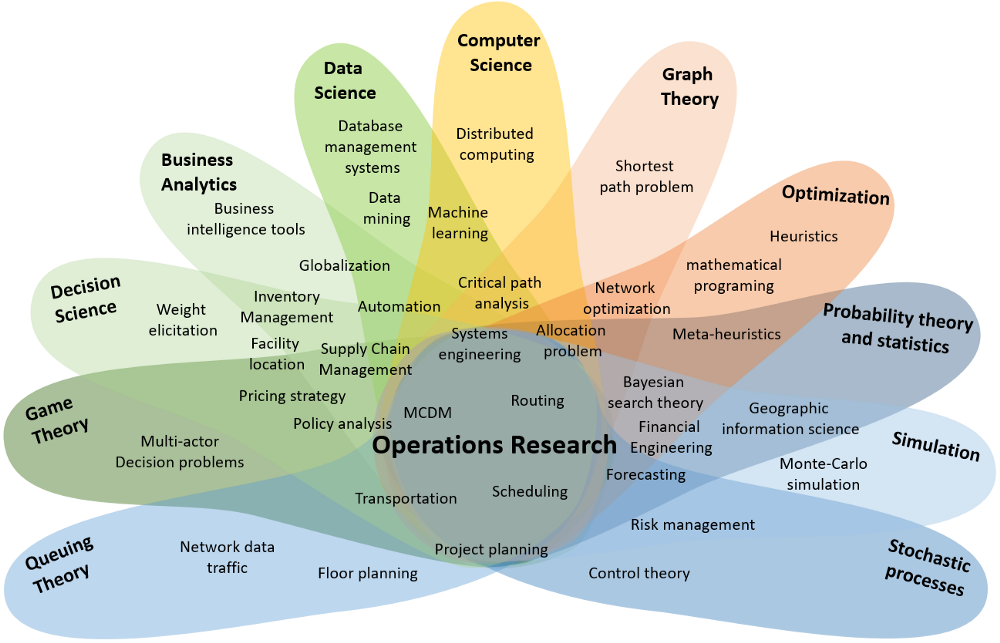
\includegraphics[width=\textwidth]{OR_AlexElkjaer.png}
  \end{center}



  \begin{itemize}
    \item OR incorporates analytical tools from many different disciplines, so that they can be applied in a rational way to help decision-makers solve problems and control operations in practice
    \item OR has been taking shape since the industrial revolution, and most notably after WWII
  \end{itemize}
  The term Operations Research was first coined in 1940 by McClosky and Trefthen
in a small town, Bowdsey, of the United Kingdom, in a military context (the Battle of England).



  \begin{itemize}
    \item A model is a simplified, idealized representation of a real object, a real process, or a real system
    \item In mathematical models, the building blocks are mathematical structures (equations, inequalities, matrices, functions and operators)
    \item Building a model:
          \tikzstyle{decision} = [diamond, draw, fill=blue!20,text width=4.5em, text badly centered, node distance=3cm, inner sep=0pt]
\tikzstyle{block} = [rectangle, draw, fill=blue!20,text width=15em, text centered, rounded corners, minimum height=3em]
\tikzstyle{line} = [draw, -latex']
\tikzstyle{cloud} = [draw, ellipse,fill=red!20, node distance=3cm,minimum height=2em]


\begin{adjustbox}{max totalsize={.9\textheight},center}

  \begin{tikzpicture}[node distance = 2cm, auto,rotate=90,transform shape]
    % Place nodes
    \node [block] (step1) {Area in need of model?};
    \node [block, below of=step1] (step2) {Controllable aspects?};
    \node [block, below of=step2] (step3) {Goals and purpose?};
    \node [block, below of=step3] (step4) {Constraints and limitations?};
    \node [block, below of=step4] (step5) {Create model};
    \node [block, below of=step5] (step6) {Collect data};
    \node [block, below of=step6] (step7) {Solve model and analyse};
    \node [coordinate, above right =1cm and 1cm of step7] (inici){};
    \node [coordinate, below right =1cm and 1cm of step4] (final){};
    % Draw edges
    \path [line] (step1) -- (step2);
    \path [line] (step2) -- (step3);
    \path [line] (step3) -- (step4);
    \path [line] (step4) -- (step5);
    \path [line] (step6) -- (step7);
    \path [line] (step7.east) -| (inici) -- (final) |- (step4.east);
  \end{tikzpicture}

\end{adjustbox}

  \end{itemize}



  \begin{itemize}
    \item The best model of a system strikes a practical compromise between being realistic vs understandable and computationally tractable
    \item Detail $\neq$ Accuracy (not all details are correct nor necessary)
    \item A too detailed model brings complexity to analyze it and exploit it
    \item Models need to be realistic and simple
  \end{itemize}
  \epigraph{``Everything should be made as simple as possible, but not simpler"}{Albert Einstein}




  \begin{itemize}
    \item Does the problem need to be solved?
    \item What is the {\it real} problem?
    \item Would the eventual solution to the problem useful for somebody?
    \item Would anybody try to implement the solution?
    \item How much of the analyst's time and cost is worth?
    \item Are there time and resources available to solve the problem?
    \item Will the solution create other serious problems for which there is no apparent remedy?
  \end{itemize}


{Problem formulation in Operational Research}

      \begin{description}
        \item[Decision variables] In what are we going to base our decision?
        \item[Objective function] How is our function build with respect to the variables?
        \item[Constraints] What are the limits in our model variables and function?
      \end{description}

      \begin{center}
        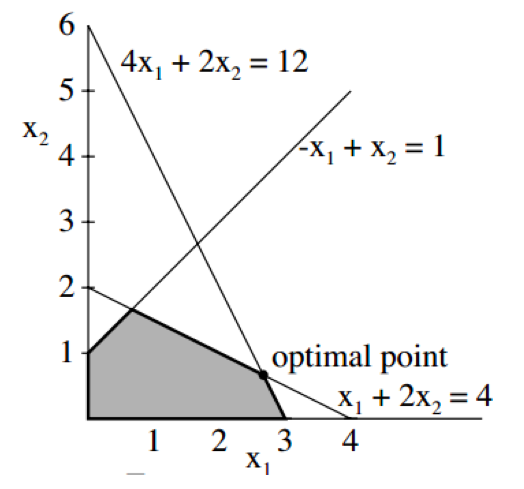
\includegraphics[width=0.8\textwidth]{LP.png}
      \end{center}




  \begin{minipage}{7cm}{Algorithm}
    Sequence of operations that can be carried out in a finite amount of time
  \end{minipage}
  \begin{itemize}
    \item It can be repeated or called recursively but it will eventually terminate.
    \item Factors influencing the execution time (unrelated to the algorthm itself):
    \begin{itemize}
      \item the programming language,
      \item the programmer's skills,
      \item the hardware being used,
      \item the task load on the computer system during execution.
    \end{itemize}
    \item The performance of an algorithm is typically linked to the size of the problem.
  \end{itemize}




      \begin{minipage}{7cm}{Class P}
        Problems that can be solved by an algorithm within an amount of computation time proportional to some polynomial function of the problem size.
      \end{minipage}
      \begin{minipage}{7cm}{Class NP}
        Problems that require computation time proportional to some exponential (or larger) function of the problem size. (The subset sum problem, for example, is $O(2^n\cdot n$))
        %https://towardsdatascience.com/how-to-find-all-solutions-to-the-subset-sum-problem-597f77677e45, incloent python program
      \end{minipage}
   
      \begin{center}
        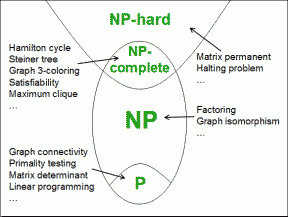
\includegraphics[scale=0.5]{nphard288.png}\\
        \footnotesize{\url{http://www.solipsys.co.uk/new/PVsNP.html}}
      \end{center}
   



  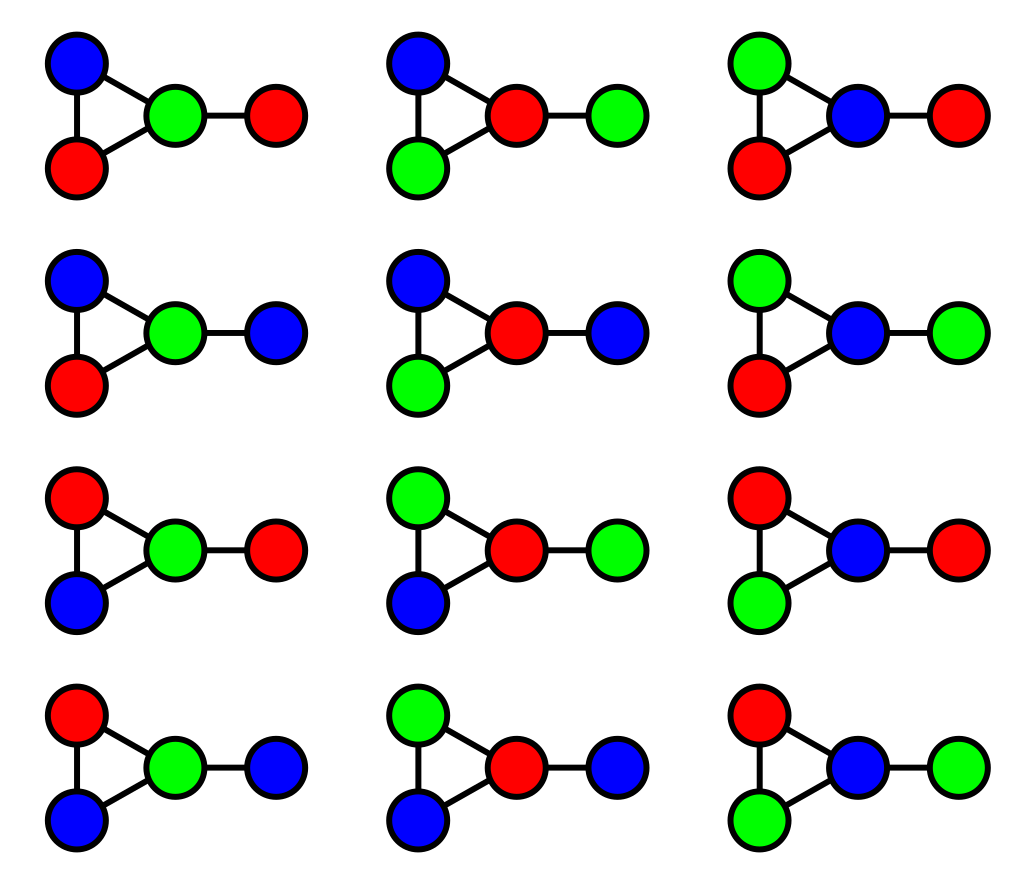
\includegraphics[width=\linewidth]{3colorproblem.png}



 
      \begin{itemize}
        \item Performance of algorithm independent of software/hardware/developer skill....? \# of computational steps.
        \item Consider worst case scenario: the largest number of steps that may be necessary.
      \end{itemize}
    
      \begin{center}
        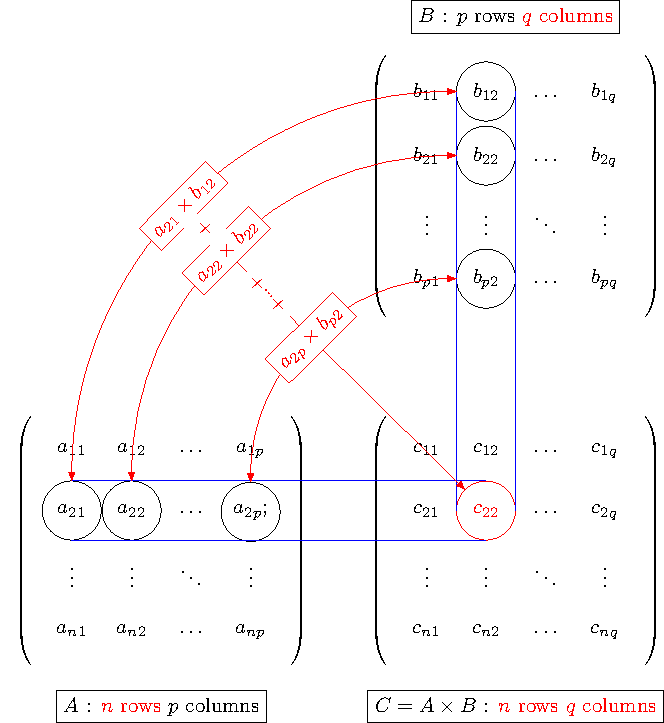
\includegraphics[width=0.7\linewidth]{matrixmultipl.pdf}
      \end{center}
      \footnotesize
      Multiplying two $n\times n$ matrices, in worst case, involves time proportional to $2n^3$.
      \normalsize
    




{Matrix multiplication is $O(n^3)$}
  \begin{footnotesize}
  \lstinputlisting[language=Python]{../code/matrixmultN3.py}
\end{footnotesize}

%--- Next Frame ---%

{$O(n)$ notation}
  \begin{itemize}
    \item We say $f(n)=O(g(n))$, and we read as "$f(n)$ is big-O of $g(n)$", if there is some $C$ and $N$ such that
    \[
      |f(n)| \leq C g(n), \; \forall n\geq N.
    \]
    In the previous example, multiplying two $n \times n$ matrices costs $2n^3=O(n^3)$ flops\footnote{FLOating Point operationS per second}. We say the algorithm is of order 3.
    \item $n$ denotes the problem size and $g(n)$ is some function of problem size.
    \item $g(n)$ is the algorithm's worst case step count, as a function of $n$.
    \item $c$ is the constant of proportionality, and accounbts for extraneous factors affecting execution time (hardware speed, programming style, computer system load during execution)
  \end{itemize}



{Different orders, different complexity}
  \begin{center}
    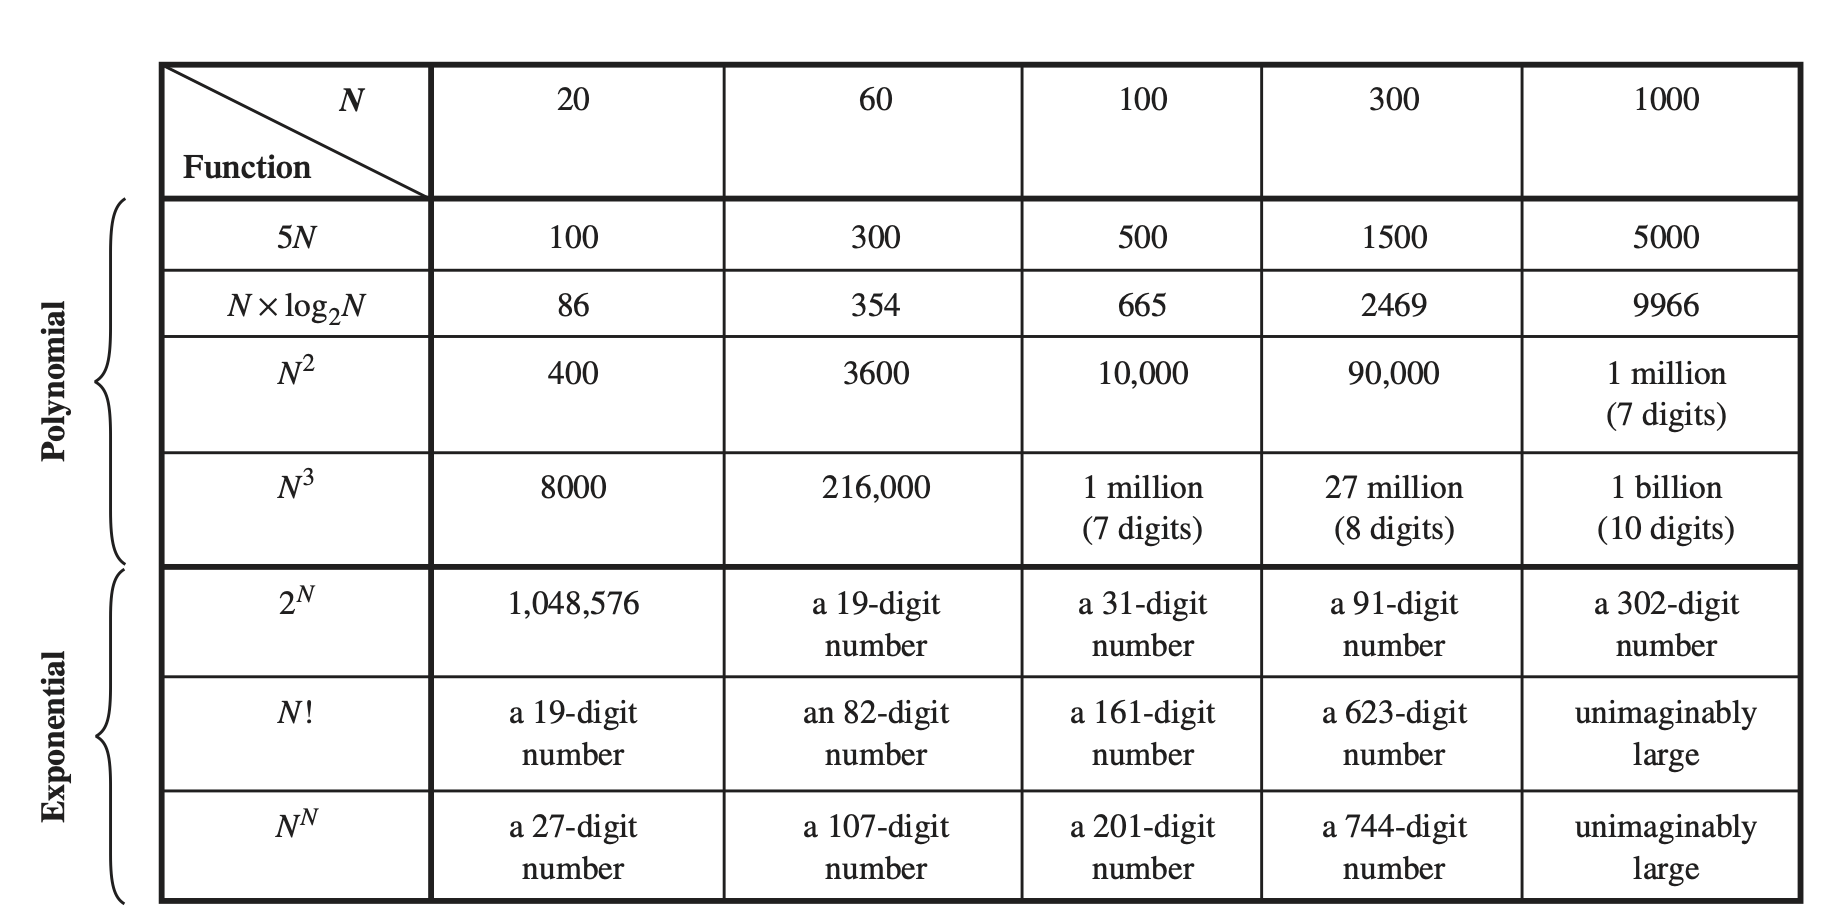
\includegraphics[width=0.8\textwidth]{Harel1.png}
  \end{center}
  Extracted from \cite{harel}


[t]{Growth rate of some functions}
 
      For comparison: the number of protons in the known universe has 79 digits; the number of nanoseconds since the Big Bang has 27 digits.\cite{harel}
   
      \begin{center}
        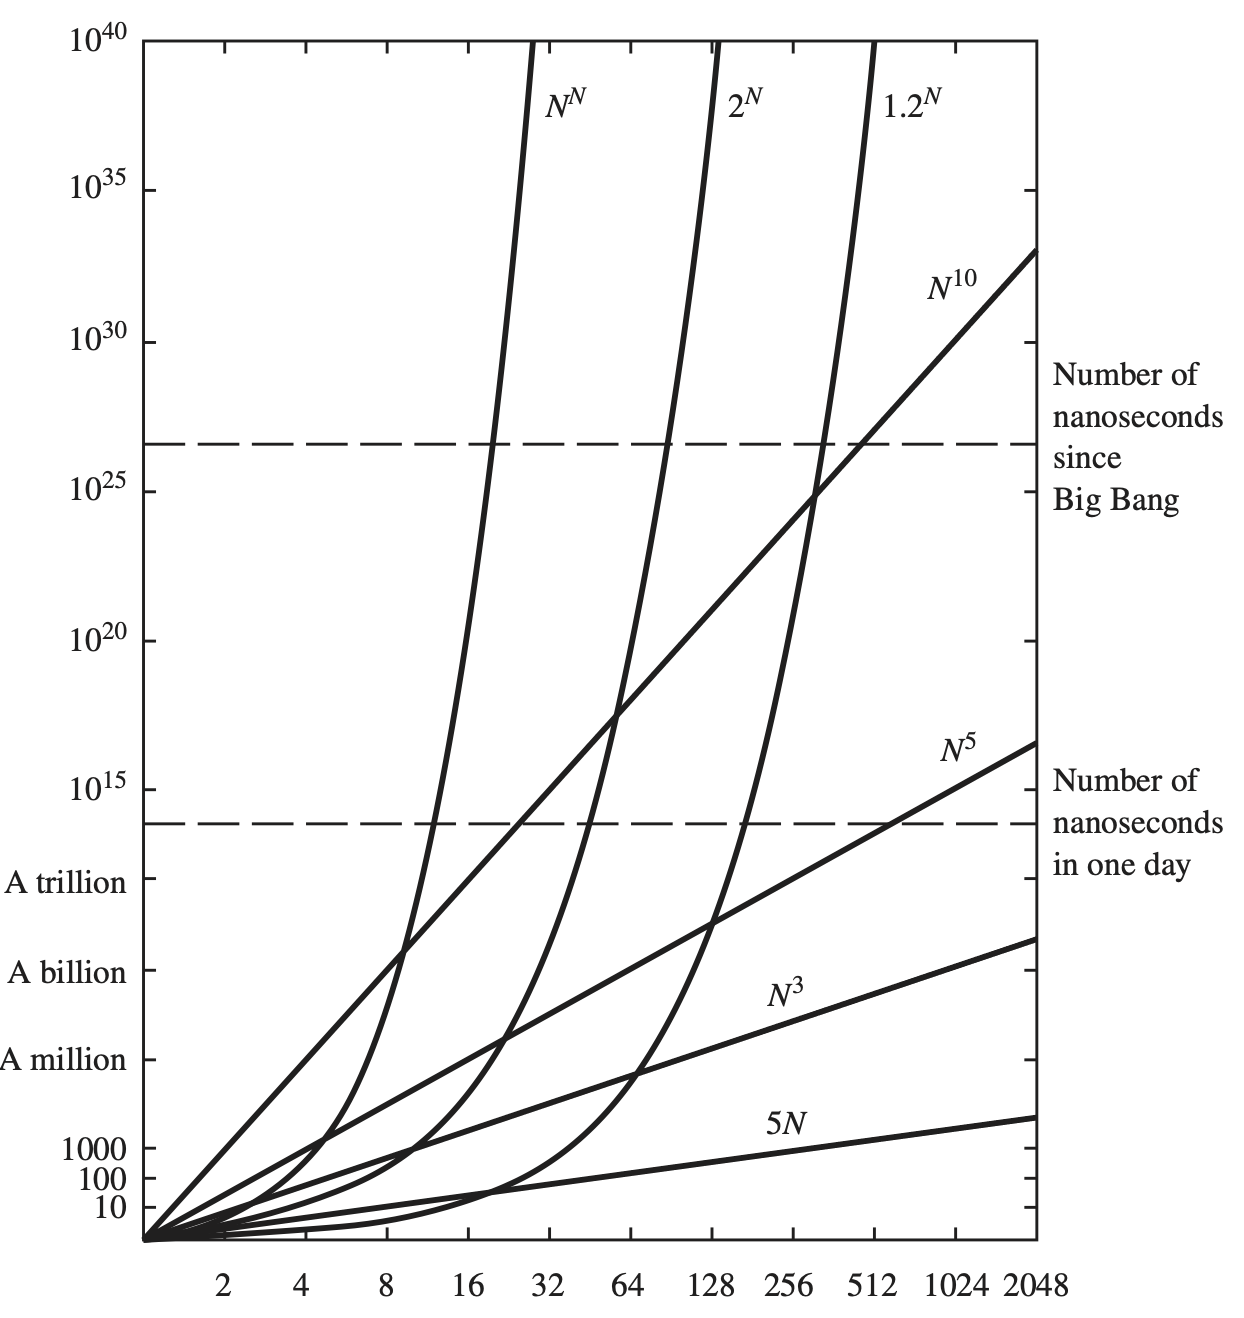
\includegraphics[width=\textwidth]{Harel2.png}
      \end{center}
 


[t]{Search space complexity: the travelling salesman problem (TSP)}
 
      \begin{itemize}
        \item A salesman must visit $n$ cities
        \item Each city must be visited just once
        \item Which path should he take to minimize the total distance travelled?
      \end{itemize}
 
      \begin{center}
        
\includegraphics[width=0.7\textwidth]{XKCD_TSP.png}
      \end{center}
      \url{https://xkcd.com/399}
 


[t]{Search space complexity: the travelling salesman problem (TSP)}
  \begin{center}
    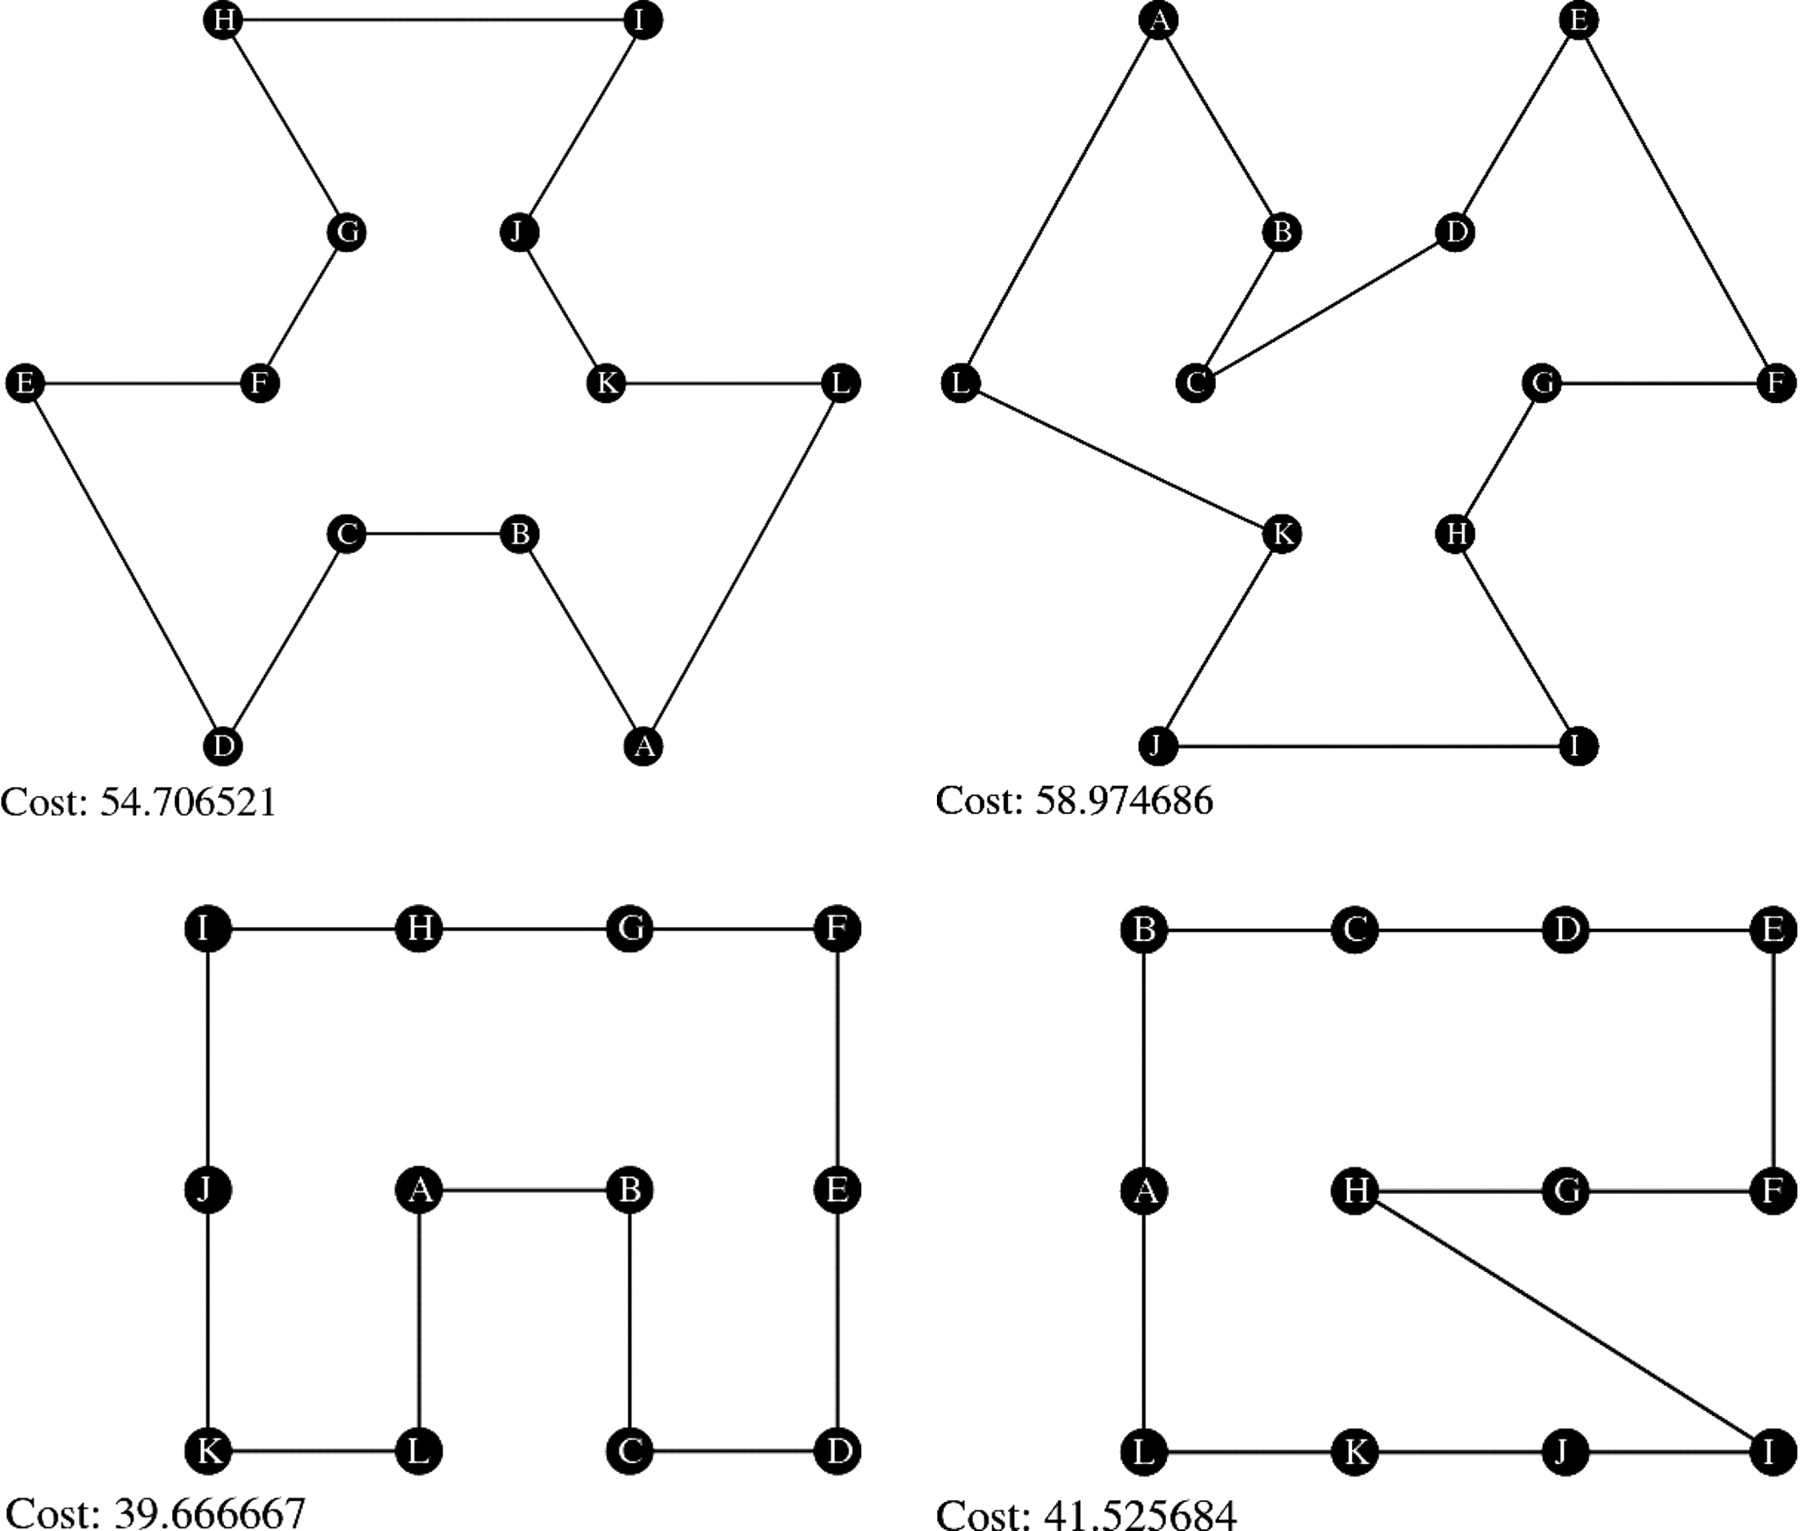
\includegraphics[width=0.5\textwidth]{TSP.jpg}
  \end{center}
  \url{https://doi.org/10.1073/pnas.0609910104}


{TSP practical example}
  Let us assume there are 4 cities and these are the "distances"\footnote{Note that the distance is not necessarily identical in both directions} between them:
  \begin{center}
  \begin{tabular}{c|cccc}
    $D_{ij}$ & city A & city B & city C & city D \\\hline
    city A & 0 & 5 & 10 & 20  \\
    city B & 10 & 0 & 35 & 20  \\
    city C & 20 & 10 & 0 & 5 \\
    city D & 10 & 5 & 10 & 0
  \end{tabular}
  \end{center}
  Check \href{https://github.com/JordiVillaFreixa/ORcourse/blob/main/code/TSPnaive.ipynb}{code} at GitHub 


{TSP practical example}
  \begin{itemize}
    \item The number of combinations is $(n-1)!$. This is the search space
    \item Asssuming a computer takes a milisecond to evaluate a solution, How long would it take for the computer to find the optimal solution in our 4 nodes problem? and how long for problems with 10, 20, 50 cities?
  \end{itemize}


{Optimality and Practicality}
  \begin{itemize}
    \item We have been trained in mathematics to find exact/perfect solutions. This is not always possible:
    \begin{itemize}
      \item Models are approximate representations of the real systems
      \item Accumulated round-off errors in computers
      \item Input data is usually approximated
      \item Exponential time algorithms require suboptimal solutions
    \end{itemize}
    \item "good enough" is not always lowering expectations, as the real world can be extremely complex.
  \end{itemize}


{Software for Operations Research}
 \begin{description}
   \item[Modeling environments] Spreadsheets (Excel, Numbers, Google), \href{https://ampl.com}{AMPL}, \href{http://www.maximalsoftware.com/mpl/}{MPL}, \href{https://www.lindo.com/index.php/products/lingo-and-optimization-modeling}{LINGO}, \href{https://www.ibm.com/docs/en/icos/12.9.0?topic=opl-optimization-programming-language}{OPL}, \href{https://www.aimms.com}{AIMMS}, \href{https://www.sas.com/es_es/software/or.html}{SAS/OR}, \href{https://support.sas.com/rnd/app/or/procedures/optmodel.html}{OPTMODEL},\href{https://www.gams.com}{GAMS}, \href{https://neos-guide.org}{NEOS}\footnote{check the \href{https://neos-guide.org/content/or}{TSP demo in NEOS/GAMS}}, ...
   \item[Solvers] \href{https://www.gurobi.com}{Gurobi},
   \href{https://www.solver.com}{Frontline Solver},
   \href{https://www.ibm.com/products/ilog-cplex-optimization-studio}{CPLEX}, ...
   \item[Software libraries] \href{https://developers.google.com/optimization}{Google OR-Tools}, \href{https://www.coin-or.org}{COIN-OR}, \href{https://www.imsl.com}{IMSL}, ...
 \end{description}
 We will be using \href{https://github.com/JordiVillaFreixa/ORcode}{Google colab} through the course when possible.


%--- Next Frame ---%
%------------------------------------------------%------------------------------------------------
%------------------------------------------------%------------------------------------------------
%------------------------------------------------%------------------------------------------------
%------------------------------------------------%------------------------------------------------
%------------------------------------------------%------------------------------------------------
%------------------------------------------------%------------------------------------------------
%------------------------------------------------%------------------------------------------------
%------------------------------------------------%------------------------------------------------
%------------------------------------------------%------------------------------------------------
%------------------------------------------------%------------------------------------------------

%----------------------------------------------------------------------------------------




\title[Introduction]{Unit 1. Introduction to Operational Research. Non linear optimization}




%%%%%%%%%%%%%%%%%%%%%%%%%%%%%%%%%%%%%%%%%%%%%%%%%%%%%%%%%%%%%%%%%%%%%%%%%%%%%
%%%%%%%%%%%%%%%%%%%%%%%%%%%%%%%%%%%%%%%%%%%%%%%%%%%%%%%%%%%%%%%%%%%%%%%%%%%%%
%%%%%%%%%%%%%%%%%%%%%%%%%%%%%%%%%%%%%%%%%%%%%%%%%%%%%%%%%%%%%%%%%%%%%%%%%%%%%

\begin{itemize}
  \item Learn about the origins and applications of Operations Research
  \item Understand system modelling principles
  \item Understand algorithm efficiency and problem complexity
  \item Contrast between the optimality and practicality
  \item Learn about software for operations Research
  \item Introduction to the Python/Colab environment
\end{itemize}

%%%%%%%%%%%%%%%%%%%%%%%%%%%%%%%%%%%%%%%%%%%%%%%%%%%%%%%%%%%%%%%%%%%%%%%%%%%%%
%%%%%%%%%%%%%%%%%%%%%%%%%%%%%%%%%%%%%%%%%%%%%%%%%%%%%%%%%%%%%%%%%%%%%%%%%%%%%
%%%%%%%%%%%%%%%%%%%%%%%%%%%%%%%%%%%%%%%%%%%%%%%%%%%%%%%%%%%%%%%%%%%%%%%%%%%%%

\section{Nonlinear optimization}
%--- Next Frame ---%
%------------------------------------------------%------------------------------------------------

  \begin{minipage}{7cm}{Production cost}

    A company aims at minimizing the production cost during a series of production periods of time $T_i$, characterised by the demand $D_ii$, equipment capacities and material limitations $E_i$, labor force $L_i$ (which cost depends quadratically on the difference of labor force between two periods $C_L(L_i-L_{i-1})^2$), productivity of each worker $P_i$, the number of units of inventory at the end of each production period $I_i$ and the cost to bring them to the next production period $C_I$.

  \begin{center}
    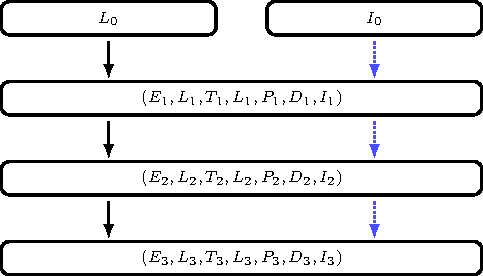
\includegraphics[width=0.4\textwidth]{ProductionSchedule.pdf}
  \end{center}
\end{minipage}

%--- Next Frame ---%
%------------------------------------------------%------------------------------------------------

  The problem, as stated, aims at minimizing the function:
  \[f(\vec{L},\vec{I})=\sum_{i=1}^T C_L (L_i-L_{i-1})^2+C_I I_i\]
  subject to:
  \[
  \begin{cases}
    L_iP_i \leq E_i\\
    I_{i-1}+L_i P_i \geq D_i\\
    I_i = I_{i-1} + L_i P_i -D_i\\
    L_i,I_i \geq 0, \; \forall i=1,\ldots,T
  \end{cases}
  \]
  Quadratic objective function with linear constraints.

%--- Next Frame ---%
%------------------------------------------------%------------------------------------------------

\begin{itemize}
  \item We want to obtain the best solution to a mathematical programming problem in which both  objective function and constraints have general non-linear forms.

  \item Most of the problems are non-linear indeed!

  \begin{itemize}
    \item Unconstrained Problems (often dealt with differential calculus)
    \item Constrained Problems (may include systems of equations to be solved)
  \end{itemize}

  \item Classical underlying mathematical theories do not necessarily provide practical methods suitable for efficient numerical computation.

  \item Points of optimality can be anywhere inside the problem boundaries

  \item No methods applicable to all non-linear problems
\end{itemize}
%--- Next Frame ---%
%------------------------------------------------%------------------------------------------------

 \begin{minipage}{7cm}{Feasible region}
   Set of points satisfying all the constraints (the area between constraint boundaries).
 \end{minipage}

 \begin{center}
  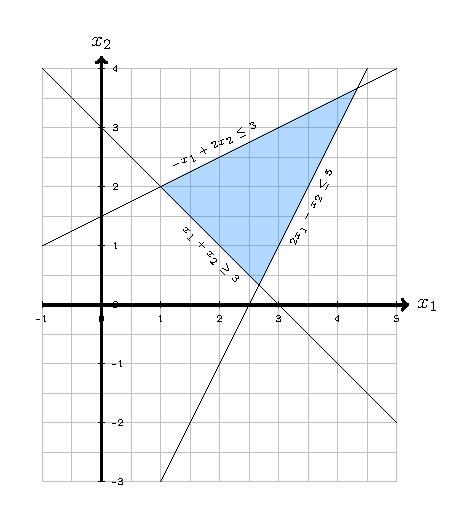
\includegraphics[width=0.6\linewidth]{feasibleregion.pdf}
 \end{center}

%--- Next Frame ---%

  \begin{center}
    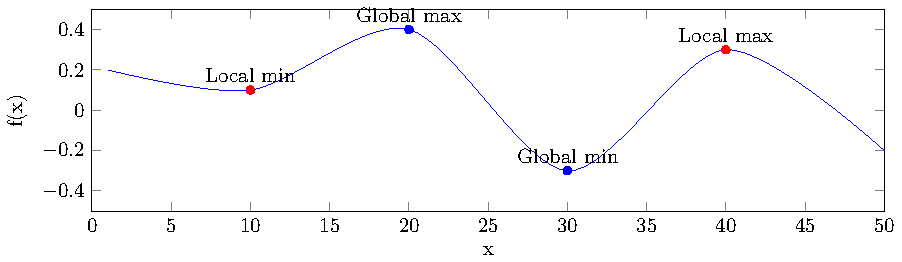
\includegraphics[width=0.6\textwidth]{globalminmax.pdf}
  \end{center}

  A local maximum of the function $f(x)$ exists in $x^*$ if there is a small positive number $\epsilon$ such that
  \[
    f(x^*)>f(x), \; \forall x\in\mathbf{R} : \|x-x^*\| < \epsilon
  \]
  A global maximum of $f(x)$ exists in $x^*$ if
  \[
    f(x^*) > f(x), \; \forall x\in\mathbf{R}
  \]
  (analogous definitions for local/global minimum)
%--- Next Frame ---%
%------------------------------------------------%------------------------------------------------

\subsection{Concavity/convexity}

  For a continuous convex function, given any two points $x_1$ and $x_2$:
  \begin{equation}
  f[\lambda x_1 +(1-\lambda)x_2] \leq \lambda f(x_1) +(1-\lambda) f(x_2), \; 0 \leq \lambda \leq 1
\label{eq:convex}
\end{equation}
    (analogous situation for a continuous concave function)
  \begin{center}
    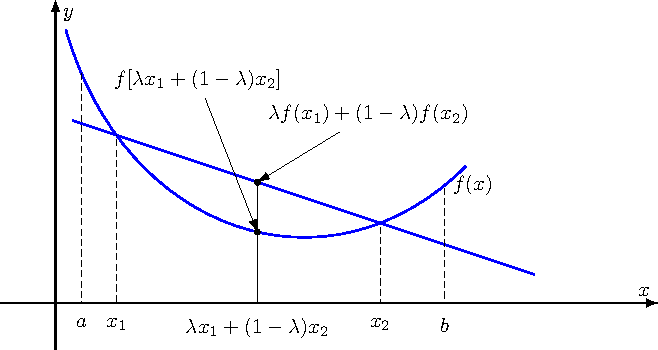
\includegraphics[width=0.6\textwidth]{concave.pdf}
  \end{center}

\begin{minipage}{7cm}{Convexity}
    The term "convex" can be applied both to sets and functions. A set $S\in \mathbf{R}^n$ is a {\it convex set} if the straight line segment connecting any two points in $S$ lies entirely inside $S$.
\end{minipage}
Note that $f(x)$ is a convex function if its domain $S$ is a convex set and if for any two points $x_1$ and $x_2$ in $S$ Eq. \ref{eq:convex} holds.

\begin{Exercise}
  Can you draw a convex function that depends on two variables, $f(x,y)$? Can you generalize Eq. \ref{eq:convex}?
\end{Exercise}


%--- Next Frame ---%
%------------------------------------------------%------------------------------------------------
  \begin{itemize}
    \item If a convex nonlinear function is to be optimized without constraints, a global minimum may occur when $f'(x)=0$. Not always this is the case:
    \begin{center}
      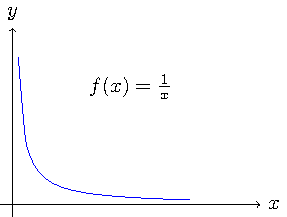
\includegraphics[width=0.5\textwidth]{1overx.pdf}
    \end{center}
    \item If the feasible region for a nonlinear programming problem is convex, each of the constraint functions is convex and are of the form $g_i(x)\leq b_i$
  \end{itemize}
%--- Next Frame ---%
%------------------------------------------------%------------------------------------------------
\begin{itemize}
    \item A local minimum is guaranteed to be a global minimum for a convex objective function in a convex feasible region, and
    \item a local maximum is guaranteed to be a global maximum for a concave objective function in a convex feasible region.
  \end{itemize}
  Many functions in nonlinear programming problems are neither concave nor convex!
  \begin{Exercise}
    Is the function $f(x)=x^2$ convex? Are the regions defined by $x^2=4$ or $x^2\geq 9$ convex?
  \end{Exercise}

    \begin{Exercise}
    Are the functions $f(x,y)=3x^2-2xy+y^2+3e^{-x}$ and $g(x,y)=x^4-8x^3+24x^2-32x+16$ convex? 
  \end{Exercise}
%--- Next Frame ---%
%------------------------------------------------%------------------------------------------------

  \begin{Exercise}
    Consider these two nonlinear problems\cite{carter}:
    \begin{center}
      \begin{tabular}{cc|cc}
        minimize & $f(x,y)=x-2xy+2y$ & minimize & $f(x,y)=x-2xy+2y$\\
        subject to & $\begin{cases}x^2+3y^2\leq10\\3x+2y\geq 1\\x,y\geq 0\end{cases}$ & 
        subject to & $\begin{cases}x^3-12x-y\geq 0\\x\geq 1\end{cases}$
      \end{tabular}
    \end{center}
    Are their feasible regions convex?
   \end{Exercise}
%--- Next Frame ---%
%------------------------------------------------%------------------------------------------------

  \begin{align}
  (\Hessian f)_{ij} &\equiv \frac{\partial^{2} f}{\partial x_{i} \partial x_{j} } \\
  \Hessian\left( \frac{x^{2}}{y} \right) &=
  \begin{bmatrix}
    \frac{2}{y} & - \frac{2x}{y^{2}} \\
    -\frac{2x}{y^{2}} & \frac{2x^{2}}{y^{3}}
  \end{bmatrix}
\end{align}

Let $f$ be a function of $n$ variables and let $1 \leq i \leq n$ and $1 \leq j \leq n$. If the partial derivatives $f'_i$ and $f'_j$ of $f$ exist in an open set $S$ containing $(x_1,\ldots, x_n)$ and both of these partial derivatives are differentiable at $(x_1, \ldots, x_n)$ then $(\Hessian f)_{ij}=(\Hessian f)_{ji}$.

\begin{itemize}
  \item If the Hessian at a given point has all positive eigenvalues, it is said to be a positive-definite matrix. This is the multivariable equivalent of “concave up” (we called it "convex" in this course).
  \item If all of the eigenvalues are negative, it is said to be a negative-definite matrix. This is like “concave down”. (we call it "concave" in this course).
  \item It the eigenvalues are mixed, you have a saddle point.
\end{itemize}

%--- Next Frame ---%
%------------------------------------------------%------------------------------------------------
\begin{Exercise}
  Study the critical points of the function $f(x,y)=4x+2y-x^2-3y^2$
\end{Exercise}


\begin{Exercise}
    Check the character of the stationary point in $(0,0)$ for the functions:
    \begin{itemize}
      \item $f(x,y)=x^2+y^2$
      \item $g(x,y)=-x^2-y^2$
      \item $h(x,y)=x^2-y^2$
      \item $k(x,y)=x^3+2y^3-xy$ (is it concave or convex in $(3,3)$? what about in $(-3,-3)$?)
    \end{itemize}

\end{Exercise}

%--- Next Frame ---%
%------------------------------------------------%------------------------------------------------
  \begin{center}
    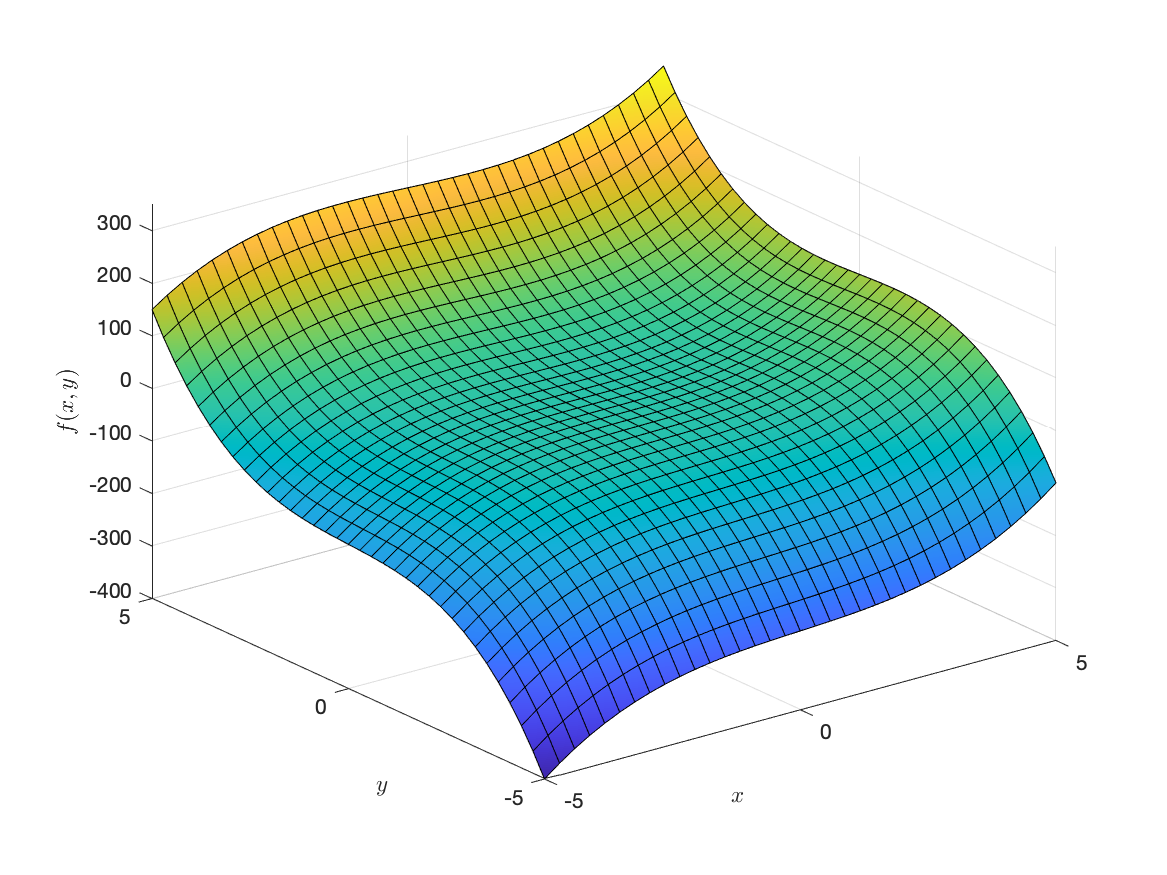
\includegraphics[width=0.8\textwidth]{../figures/x3plus2y3minusxy.png}
  \end{center}

%--- Next Frame ---%
%------------------------------------------------%------------------------------------------------
  For unconstrained problems with just one variable $x$, if first and second derivatives exist in $x^*$:
  \begin{description}
    \item[Necessary conditions] If $\frac{df}{dx}=0$ at $x=x^*$
    \begin{itemize}
      \item $\frac{d^2f}{dx^2}\geq 0$, for a local minimum at $x=x^*$
      \item $\frac{d^2f}{dx^2}\leq 0$, for a local maximum at $x=x^*$
    \end{itemize}
    \item[Sufficient conditions] If $\frac{df}{dx}=0$ at $x=x^*$
    \begin{itemize}
      \item $\frac{d^2f}{dx^2}> 0$, for a local minimum at $x=x^*$
      \item $\frac{d^2f}{dx^2}< 0$, for a local maximum at $x=x^*$
    \end{itemize}
  \end{description}
%--- Next Frame ---%
%--- Next Frame ---%
%------------------------------------------------%------------------------------------------------
  For unconstrained problems with several variables $\uvec{x}=(x_1,\ldots,x_n)$:
  \begin{description}
    \item[Sufficient condition] If $\pdv{f}{x_i}=0$ at $\uvec{x}=\uvec{x}^*$:
    \begin{itemize}
      \item $\grad{f}=\uvec{0}$, for a local minimum at $x=x^*$ if the function is convex;
      \item $\grad{f}=\uvec{0}$, for a local maximum at $x=x^*$ if the function is concave.
    \end{itemize}
    \item[Decision conditions] The function $f$ is a convex function if $H_f$ is positive definite or positive semidefinite for all $\uvec{x}$; and $f$ is concave if $H_f$ is negative definite or negative semidefinite for all $\uvec{x}$. For $f:\mathbf{R}^2\rightarrow\mathbf{R}$
    \[
      {\mathbf H}_f(x,y)=\begin{pmatrix} \frac{\partial^2 f}{\partial x^2} & \frac{\partial^2 f}{\partial x \partial y} \\ \frac{\partial^2 f}{\partial y \partial x} & \frac{\partial^2 f}{\partial y^2}\end{pmatrix} =
      \begin{pmatrix} A & C \\ C & B \end{pmatrix}
\]
  \end{description}

  Let $f$ be a twice-differentiable function of many variables on the convex open set $S$ and denote the Hessian of $f$ at the point $x$ by $H(x)$. Then
\begin{itemize}
  \item $f$ is concave if and only if $H(x)$ is negative semidefinite $\forall x \in S$
  \item if $H(x)$ is negative definite $\forall x \in S$ then $f$ is strictly concave (see Eq. \ref{eq:convex})
  \item $f$ is convex if and only if $H(x)$ is positive semidefinite $\forall x \in S$
  \item if $H(x)$ is positive definite $\forall x \in S$ then $f$ is strictly convex (see Eq. \ref{eq:convex})
\end{itemize}

%--- Next Frame ---%
%------------------------------------------------%------------------------------------------------
  Things are not so simple if, for example, functions are not derivable in $x^*$:
  \begin{center}
    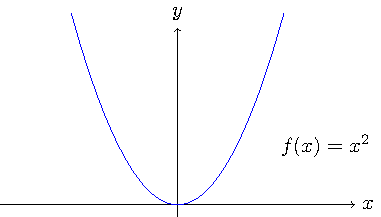
\includegraphics[width=0.4\textwidth]{x2.pdf}
    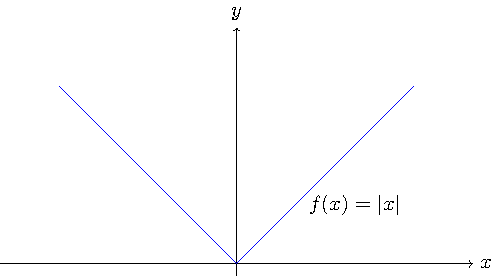
\includegraphics[width=0.4\textwidth]{absx.pdf}
  \end{center}
  Or, if the function is not convex (nor concave), the sufficient condition is lost and we may find local optimal points, instead of global.

  For constrained optimization problems, the shape of the feasible region adds difficulty.



%--- Next Frame ---%
%------------------------------------------------%------------------------------------------------
\subsection{Iterative methods}

Let us assume a concave function. First, establish error tolerance $\epsilon$. Then:
  \begin{enumerate}
    \item Set up lower and upper bounds for $x$ by finding $x_l,x_u$ such that $\frac{df}{dx_l}\geq 0$ and $\frac{df}{dx_u}\leq 0$
    \item Get new trial intermediate solution (eg, $x=\frac{x_l+x_u}{2}$)
    \item If $x_u-x_l\leq \epsilon$, then terminate
    \item If $\frac{df}{dx}\geq 0$, set $x_l=x$; if $\frac{df}{dx}\leq 0$, set $x_u=x$
    \item Go to step 1
  \end{enumerate}

  For an implementation, see \href{https://machinelearningmastery.com/line-search-optimization-with-python/}{this link}
%--- Next Frame ---%
%------------------------------------------------%------------------------------------------------
For a continuous function it guarantees to find an extremum.

\begin{minipage}{7cm}{Golden ratio}
   Two quantities are in the golden ratio if their ratio is the same as the ratio of their sum to the larger of the two quantities:
\[
\frac{a+b}{a}=\frac{a}{b}=\psi \Rightarrow \psi=\frac{1+\sqrt{5}}{2}=1.616033988...
\]
\end{minipage}

Procedure of the Golden search method, given a function  to be minimized, $f(x)$, the interval to be searched as $x\in(x_1,x_4)$, and their functional values $f(x_1)$ and $f(x_2)$:
\begin{enumerate}
  \item Calculate an interior point and its functional value $f(x_3$). Ensure the position of $x_3$ follows the golden ratio between the distances $\frac{x_2-x_1}{x_3-x_1}=\frac{x_3-x_1}{x_2-x_3}=\psi$.
  \item Using the triplet, determine if convergence criteria are fulfilled. If they are, estimate the $x$ at the minimum from that triplet and terminate/return.
  \item Select $x_4$ within the largest interval, following the same ratios as in Step 1.
  \item The three points for the next iteration will be the one where $f(x)$ is a minimum, and the two points closest to it in $x$.
  \item Go to step 2.
\end{enumerate}

\begin{Exercise}
  Use the Golden Search method to find the minimum of function $f(x)=x^2-6x+15$ in the interval $x\in(0,10)$. Set up a spreadsheet to do so.
  %https://www.youtube.com/watch?v=hLm8xfwWYPw
\end{Exercise}


%--- Next Frame ---%
%------------------------------------------------%------------------------------------------------
\begin{program}
  E2. Build a Python code that can run one-dimensional search algorithms for user defined functions, using or not first derivatives. Implement the one-dimensional line search and the golden search algorithms and find the optimal solution for the functions:
  \begin{itemize}
    \item $f(x)=x^4-16x^3+45 x^2-20x+203$ within the range $x\in(2.5,14)$
    \item $g(x)=x^5-2x^4-23x^3-12x^2+36x$ within the range $x\in(2,3)$
  \end{itemize}
  Try both a direct implementation as well as the use of solvers in scipy.
\end{program}

\begin{Exercise}
  Draw the {\em Rosenbruck's function}, $f(x,y)=100(y-x^2)^2+(1-x)^2$ and discuss on its convexity, the feasibility of its minimization and the most appropriate numerical method to use.
\end{Exercise}


%--- Next Frame ---%
%------------------------------------------------%------------------------------------------------

%https://suzyahyah.github.io/calculus/optimization/2018/04/06/Taylor-Series-Newtons-Method.html
  As a reference (not the central aim of this course) here is a list of some algorithms/methods to explore to perform unconstrained optimization in multiple dimensions:
  \begin{itemize}
    \item Newton's method,
    \item Quasi-Newton methods (e.g., \href{https://machinelearningmastery.com/bfgs-optimization-in-python/}{BFGS}),
    \item Trust-region methods,
    \item \href{https://en.wikipedia.org/wiki/Conjugate_gradient_method}{Conjugated gradient methods}.
  \end{itemize}
  and their many variants.


\subsection{Constrained optimization}
%--- Next Frame ---%
%------------------------------------------------%------------------------------------------------
In the previous section we have considered functions of several variables that are independent from each other. What happens if the variables are, however, not independent from each other? (see excellent material in \href{https://www.statslab.cam.ac.uk/~rrw1/}{Richard Weber's web site})

  \begin{center}
    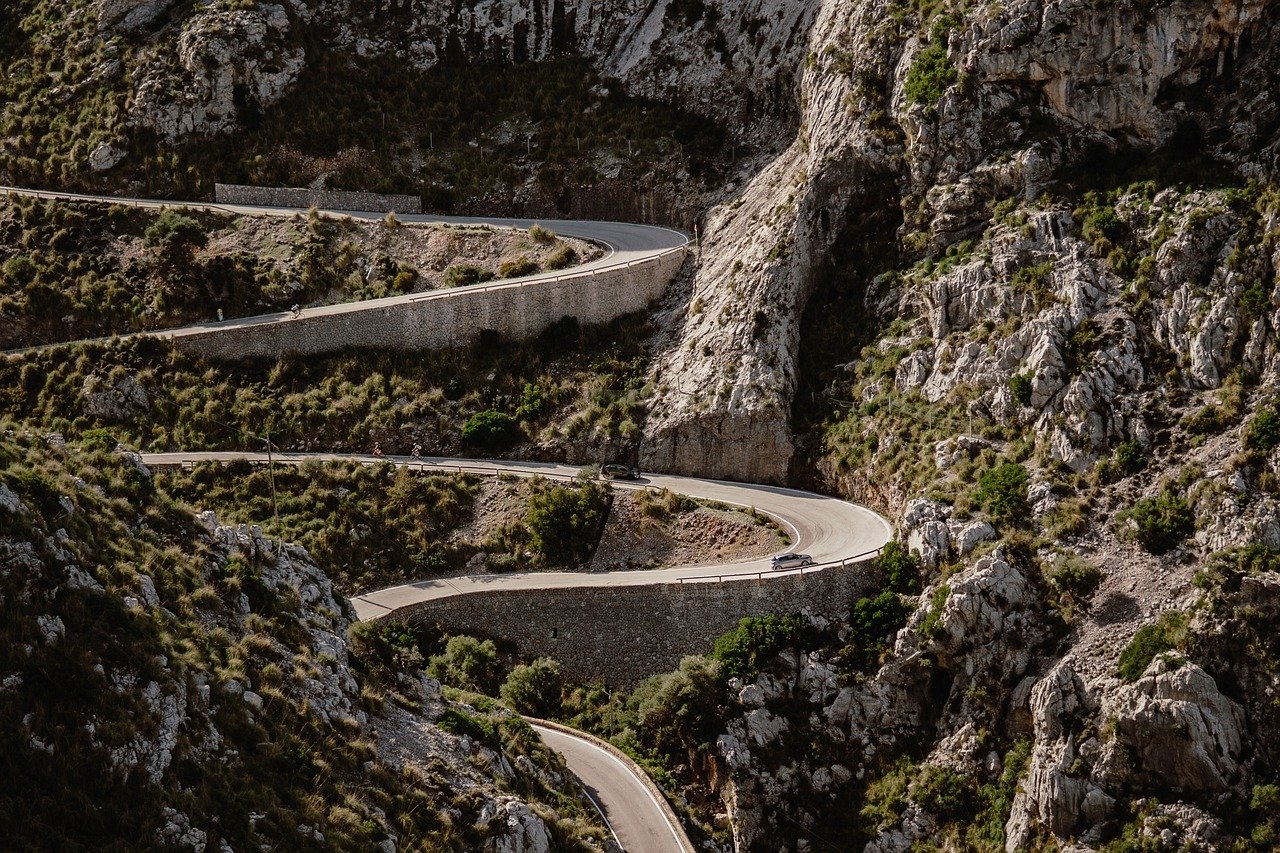
\includegraphics[width=0.7\textwidth]{../figures/mallorca.jpg}\newline
    What is the maximum height we can attain constrained to the trajectory of the road?
  \end{center}

%--- Next Frame ---%
%------------------------------------------------%------------------------------------------------
  Let us consider optimizing a function $f(x,y)$ (the height of the hill in the previous exemple) subject to the constrain $g(x,y)=c$ (the equation describing the path, the road).

  One can simply substitute $g(x,y)=c$ in $f(x,y)$, but this may not involve trivial algebra.

  Alternatively, let us consider the method of the Lagrange multipliers. To optimize $f(x,y)$ we require
  \[
    df=\frac{\partial f}{\partial x} dx +\frac{\partial f}{\partial y}dy=0
  \]
  we saw that if $dx$ and $dy$ were independent, $\frac{\partial f}{\partial x}=\frac{\partial f}{\partial y}=0$. But they are not here: they are constrained by $g(x,y)$, which is a constant:
  \[
    dg=\frac{\partial g}{\partial x} dx +\frac{\partial g}{\partial y}dy=0
  \]
  Let us consider a parameter $\lambda$ (the {\it Lagrange multiplier}) and obtain an expression for which $dx$ and $dy$ are independent:
  \[
    d(f+\lambda g)=(\frac{\partial f}{\partial x}+\lambda \frac{\partial g}{\partial x}) dx +(\frac{\partial f}{\partial y}+\lambda \frac{\partial g}{\partial y})dy=0
  \]
  Now:
  \begin{eqnarray*}
    \frac{\partial f}{\partial x}+\lambda \frac{\partial g}{\partial x} &=&0\\
    \frac{\partial f}{\partial y}+\lambda \frac{\partial g}{\partial y} &=&0\\
    g(x,y)&=&c
  \end{eqnarray*}
  are sufficient to find $\lambda$, $x^*$ and $y^*$.

%--- Next Frame ---%
%------------------------------------------------%------------------------------------------------
  \begin{center}
  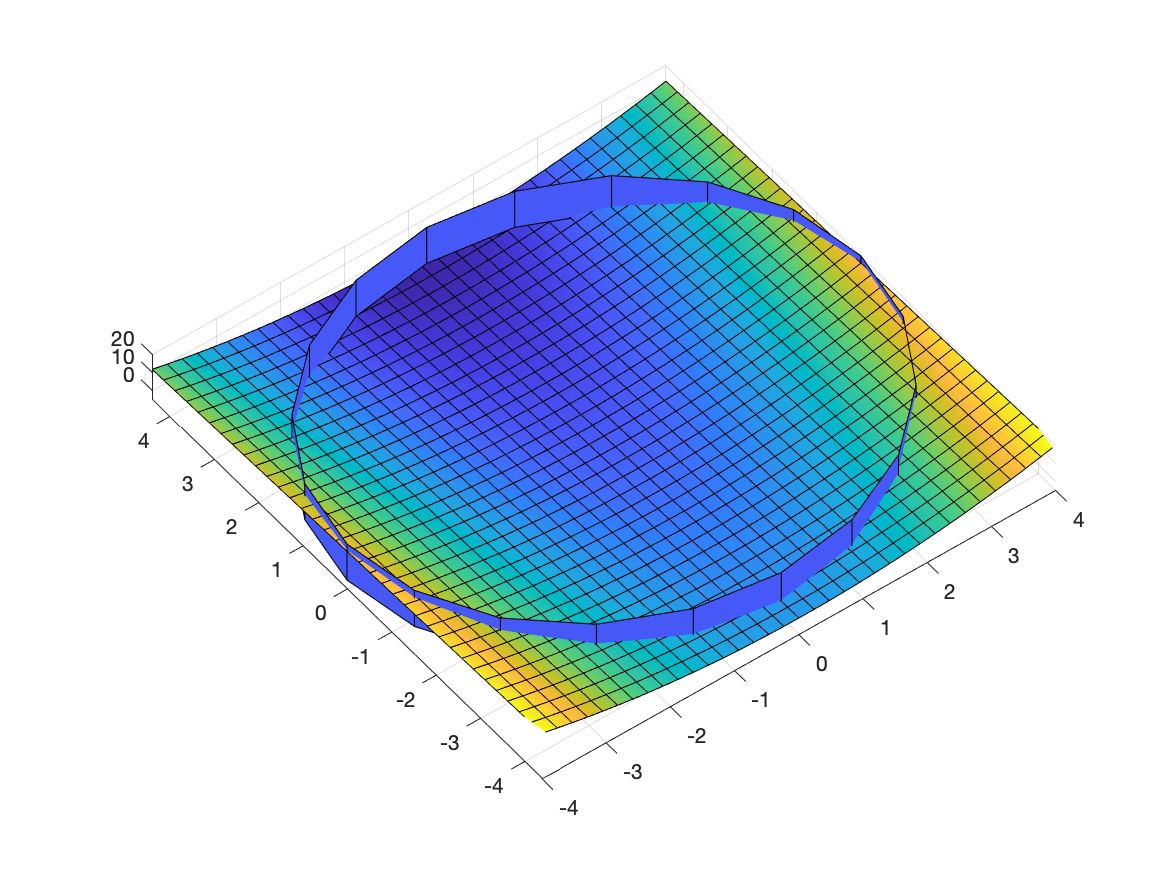
\includegraphics[width=0.4\textwidth]{../figures/Lagrangex2minusy.png}
  \end{center}
  \begin{Exercise}
  Find the optimal values of the function $f(x,y)=x^2-y$ constrained within the circumference $x^2+y^2=4$. (note that, interestingly, in the optimal value $x^*$ we will get a gradient for the constraint that is parallel to the gradient of the function: $\grad f(x^*)=\lambda^* \grad g(x^*)$).
\end{Exercise}
%--- Next Frame ---%
%------------------------------------------------%------------------------------------------------
  The general problem we study takes the form
  \begin{center}
  \begin{tabular}{cc}
    maximize & $f(x)$ \\
    subject to & $\begin{cases}x\in X\\g(x)=b\end{cases}$
  \end{tabular}
\end{center}
where
  \begin{center}
  \begin{tabular}{rl}
    $x \in \mathbf{R}^n$ & ($n$ decision variables)\\
    $f: \mathbf{R}^n \rightarrow \mathbf{R}$ & (objective function)\\
    $X \subseteq  \mathbf{R}^n$ & (regional constraints) \\
    $\begin{rcases}
      g: \mathbf{R}^n \rightarrow \mathbf{R}^m\\
      b \subseteq \mathbf{R}^m
    \end{rcases}$ & ($m$ functional constraints)\\
  \end{tabular}
\end{center}
If the constraint is $g(x)\leq b$ we introduce a {\bf slack variable} $z$ and write:
\[g(x)+z=b, \, z\geq0\]
Regional and functional constraints define the {\bf feasible set} for $x$

%--- Next Frame ---%
%------------------------------------------------%------------------------------------------------

  In the Lagrange approach, the constrained maximization (minimization) problem is rewritten as a Lagrange function 
  
  \[L(x,\lambda)=f(x)-\lambda g(x)\]
  
  whose optimal point is a saddle point, i.e. a global maximum (minimum) over the domain of the choice variables and a global minimum (maximum) over the multipliers.

  Let us take this example:
  \begin{center}
  \begin{tabular}{cc}
    maximize & $f(x)=x_1-x_2-2x_3$ \\
    subject to & $\begin{cases}x_1+x_2+x_3=5\\x_1^2+x_2^2=4\\x=(x_1,x_2,x_3)\in \mathbf{R}^3\end{cases}$
  \end{tabular}
\end{center}
\begin{enumerate}
  \item We write the Lagrangian as (note we have two constraints):
  \begin{eqnarray*}
    L(x,\lambda)&=&x_1-x_2-2x_3-\lambda_1 (x_1+x_2+x_3-5)-\lambda_2(x_1^2+x_2^2-4)\\
    &=& [x_1(1-\lambda_1)-\lambda_2x_1^2]+[x_2(-1-\lambda_1)-\lambda_2x_2^2]+[x_3(-2-\lambda_1)]\\
    &&+5\lambda_1+4\lambda_2
  \end{eqnarray*}
  \item We want to minimize the Lagrangian subject to the regional constraints $x=(x_1,x_2,x_3)\in \mathbf{R}^3$.
  \item We find the values $\lambda$ such that will define a feasible set
  \[
  Y=\left\{\lambda: \underbrace{\mathrm{min}}_{x\in  \mathbf{R}^3} L(x,\lambda) >-\infty \right\}
  \]
  So, we only consider the values of $\lambda$ for which we obtain a finite minimum. In the example
  \[
  Y=\left\{\lambda: \lambda_1=-2, \lambda_2<0 \right\}
  \]
  \item For $\lambda \in Y$, the minimum will be obtained at some $x(\lambda)$ (that depends on $\lambda$ in general). Here, $x(\lambda)=(3/2\lambda_2,1/2\lambda_2,x_3)^T$.
  \item Finally, we find a $\lambda$ value that provides a feasible value $x(\lambda)$. Here
  \[
    x_1^2+x_2^2=4 \Rightarrow \lambda_2 = -\sqrt{5/8}
  \]
  So, $x^*$ is optimal:
  \[
    x^* =(-3\sqrt{2/5},-\sqrt{2/5},5+4\sqrt{2/5})^T; \, \lambda^*=(-2,-\sqrt{5/8})^T
  \]
\end{enumerate}


\begin{Exercise}
  Use the Lagrange multipliers to solve this problem:
  \begin{center}
    \begin{tabular}{cc}
      minimize & $f(x,y)=x^2y$ \\
      subject to & $x^2+y^2=1$
    \end{tabular}
  \end{center}
\end{Exercise}
%--- Next Frame ---%
%------------------------------------------------%------------------------------------------------
% https://en.wikipedia.org/wiki/Karush%E2%80%93Kuhn%E2%80%93Tucker_conditions
  \note[item]{\url{https://people.maths.bris.ac.uk/~maxmr/opt/kt1.pdf}}
  \note[item]{\url{https://www.cmi.ac.in/~madhavan/courses/dmml2018/literature/Lagrangian_Methods_for_Constrained_Optimization.pdf}}

  Let us consider a general optimization problem with constraints: let $f:\mathbf{R}^n \rightarrow \mathbf{R}$ be the objective function and $\uvec{g}:\mathbf{R}^n \rightarrow \mathbf{R}^m$ a set of constraint functions ($\uvec{g}(\uvec{x})=(g_1(\uvec{x}),\ldots,g_m(\uvec{x}))$ with $\uvec{x}=(x_1,\ldots,x_n)$. We want to obtain
  \begin{center}
  Min $f(\uvec{x})$ such that $\uvec{g}(\uvec{x})\geq 0$
\end{center}
  \begin{theorem}
    If $\uvec{x}^*$ is a local minimum for the optimisation problem and the constraints $\uvec{g}(\uvec{x})\geq 0$ are satisfied at $\uvec{x}^*$, then $\uvec{x}^*$ must satisfy:
    \begin{eqnarray*}
      \grad f({\uvec{x}})&=&\lambda_1 \grad g_1(\uvec{x})+\cdots+\lambda_m \grad g_m(\uvec{x})\\
      0&=&\lambda_1  g_1(\uvec{x})=\cdots=\lambda_m  g_m(\uvec{x})\\
      0&\leq&\uvec{g}(\uvec{x})
    \end{eqnarray*}
  \end{theorem}

%--- Next Frame ---%
%------------------------------------------------%------------------------------------------------


  \begin{Exercise}
     Consider this NLO problem\cite{carter}:
    \begin{center}
     \begin{tabular}{cc}
      maximize & $f(x,y)=x^2y+2y^2$ \\
      subject to & $\begin{cases}x+3y\leq 9\\x+2y\leq 8\\3x+2y\leq 18\\0\leq x \leq 5\\0\leq y \leq 2\end{cases}$
    \end{tabular}
  \end{center}
    Solve the program graphically- Begin at point $(0,0)$ and check the gradient. Check the KKT conditions. If they are not satisfied, find an improving direction in the feasible region.
  \end{Exercise}


%--- Next Frame ---%
%------------------------------------------------%------------------------------------------------
  To better understand these exercises, you can make use of \href{https://www.geogebra.org/3d?lang=en}{geogebra}.
\begin{Exercise}
  Is it possible to maximize $f(x,y)=xy$ subject to $100 \geq x+y$ and $x\leq 40$?
  % solution: not necessarily, feasible region is not bound. In fact it is not possible
\end{Exercise}
\begin{Exercise}
  %https://personal.math.ubc.ca/~israel/m340/kkt2.pdf
  What about maximizing $f(x,y)=xy$ subject to $x+y^2\leq 2$ and $x,y \geq 0$?
\end{Exercise}
%https://www.sfu.ca/~wainwrig/Econ400/lecture-notes-Kuhntucker.pdf

%------------------------------------------------%------------------------------------------------

%----------------------------------------------------------------------------------------




\title[Introduction]{Unit 2. Linear programming. Introduction}



%%%%%%%%%%%%%%%%%%%%%%%%%%%%%%%%%%%%%%%%%%%%%%%%%%%%%%%%%%%%%%%%%%%%%%%%%%%%%
%%%%%%%%%%%%%%%%%%%%%%%%%%%%%%%%%%%%%%%%%%%%%%%%%%%%%%%%%%%%%%%%%%%%%%%%%%%%%
%%%%%%%%%%%%%%%%%%%%%%%%%%%%%%%%%%%%%%%%%%%%%%%%%%%%%%%%%%%%%%%%%%%%%%%%%%%%%

\begin{itemize}
  \item Learn how to formulate a linear programming model
  \item Get familiar with the terms feasible region, feasiblke solutions and optimal feasible solutions
  \item Managing graphical solution of the linear programming model
  \item Identify models with unique, multiple or no optimal feasible solutions
  \item Introducing the Simplex method
\end{itemize}

\section{Introduction to linear programming}


  \begin{minipage}{7cm}{Linear programming}
    Linear programs have a linear objective function and linear constraints, which may
    include both equalities and inequalities. The feasible set is a polytope, that is, a convex,
    connected set with flat, polygonal faces. The contours of the objective function are planar.
   \cite{nocedal}
  \end{minipage}
  A wide variety of applications can be modeled with linear programming.


  Steps:
\begin{enumerate}
  \item identify the controllable decision variables $x_i$, with $i=1,\ldots,n$.
  \item establish the objective criterion: to either maximize or minimize some function of the form:
  \[
    z = c_1 x_1 +\cdots + c_n x_n = \sum_{i=1}^n c_i x_i
  \]
  where $c_i$ represents problem dependent constants.
  \item resource limitations and bounds on decision variables as linear equations or inequalities like
  \[
     a_1 x_1 +\cdots + a_n x_n \leq b
  \]
\end{enumerate}

  \begin{center}
    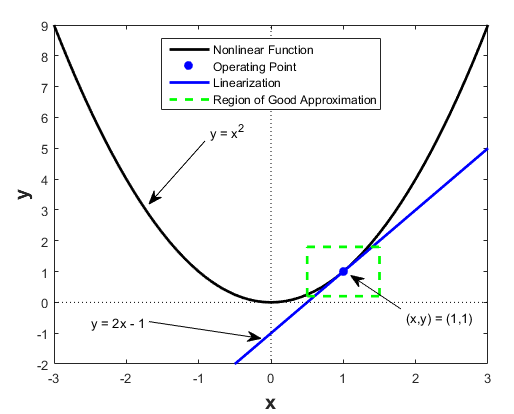
\includegraphics[width=0.45\linewidth]{linearization}
    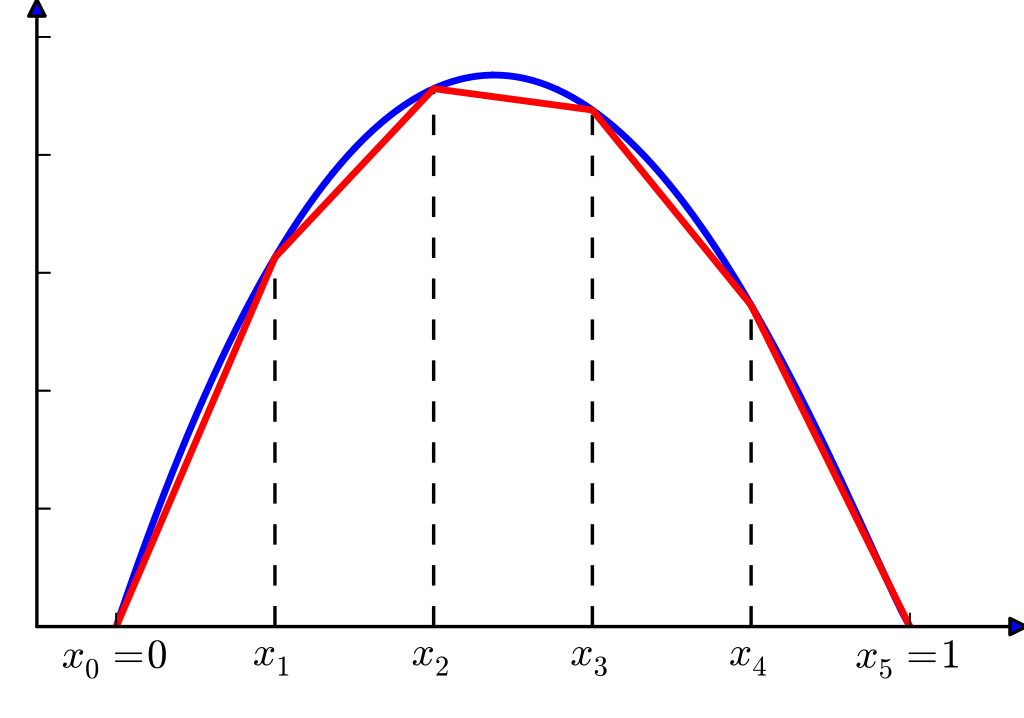
\includegraphics[width=0.45\linewidth]{PWLapprox}

  \href{https://es.mathworks.com/help/slcontrol/ug/linearizing-nonlinear-models.html}{Matlab example}
  \end{center}

  \begin{Exercise}
    A manufacturer of computer system components assembles two models of wireless routers, model A and model B. The amounts of materials and labor required for each assembly, and the total amounts available, are shown in the following table. The profits that can be realized from the sale of each router are \$22 and \$28 for models A and B, respectively, and we assume there is a market for as many routers as can be manufactured.\cite{carter}
    \begin{center}
    \begin{tabular}{cccc}
      & Resources  & Resources  B & Resources  \\
      & per Unit A &  per Unit B &  available \\\hline
      Materials & 8 & 10 & 3400\\
      Labor & 2 & 3 & 960\\\hline
    \end{tabular}
  \end{center}
  How to maximize the benefits?
  \end{Exercise}
  \begin{equation*}
    \begin{aligned}
      \text{maximize } \quad & z = 22 x_A+28x_B \\
      \text{subject to }\quad &
      \begin{array}{rcl}
        8x_A+10x_B &\leq &3400 \\
        2x_A+3x_B &\leq &960 \\
        x_A &\geq &0 \\
        x_B &\geq& 0
      \end{array}
    \end{aligned}
  \end{equation*}


  \begin{Exercise}
  A company wishes to minimize its combined costs of production and inventory over a four-week time period. An item produced in a given week is available for consumption during that week, or it may be kept in inventory for use in later weeks. Initial inventory at the beginning of week 1 is 250 units. The minimum allowed inventory carried from one week to the next is 50 units. Unit production cost is \$15, and the cost of storing a unit from one week to the next is \$3. The following table shows production capacities and the demands that must be met during each week.\cite{carter}
    \begin{center}
    \begin{tabular}{ccc}
      Period  & Production capacity & Demand  \\\hline
      1 &  800 &  900 \\
      2 & 700 & 600\\
      3 & 600 & 800\\
      4 & 800 & 600
    \end{tabular}
  \end{center}
  A minimum production of 500 items per week must be maintained. Inventory costs are not applied to items remaining at the end of the fourth production period, nor is the minimum inventory restriction applied after this final period.
  \end{Exercise}
  Let $x_i$ be the number of units produced during the $i^{th}$ week, for $i = 1, …, 4$. The formulation is somewhat more manageable if we let $A_i$ denote the number of items remaining at the end of each week (accounting for those held over from previous weeks, those produced during the current week, and those consumed during the current week). Note that the $A_i$ values are not decision variables, but merely serve to simplify our written formulation. Thus,
  \begin{eqnarray*}
    A_1&=&250+x_1-900\\
    A_2&=&A_1+x_2-600\\
    A_3&=&A_2+x_3-800\\
    A_4&=&A_3+x_4-600
  \end{eqnarray*}
  \begin{equation*}
    \begin{aligned}
      \text{minimize } \quad & z = 15\cdot(x_1+x_2+x_3+x_4)+3\cdot (A_1+A_2+A_3) \\
      \text{subject to }\quad &
      \begin{array}{c}
        500 \leq x_1 \leq 700\\
        500 \leq x_2 \leq 700\\
        500 \leq x_3 \leq 600\\
        500 \leq x_4 \leq 800\\
        x_i \geq 0, \, i=1,2,3,4
      \end{array}
    \end{aligned}
  \end{equation*}


  \begin{center}
    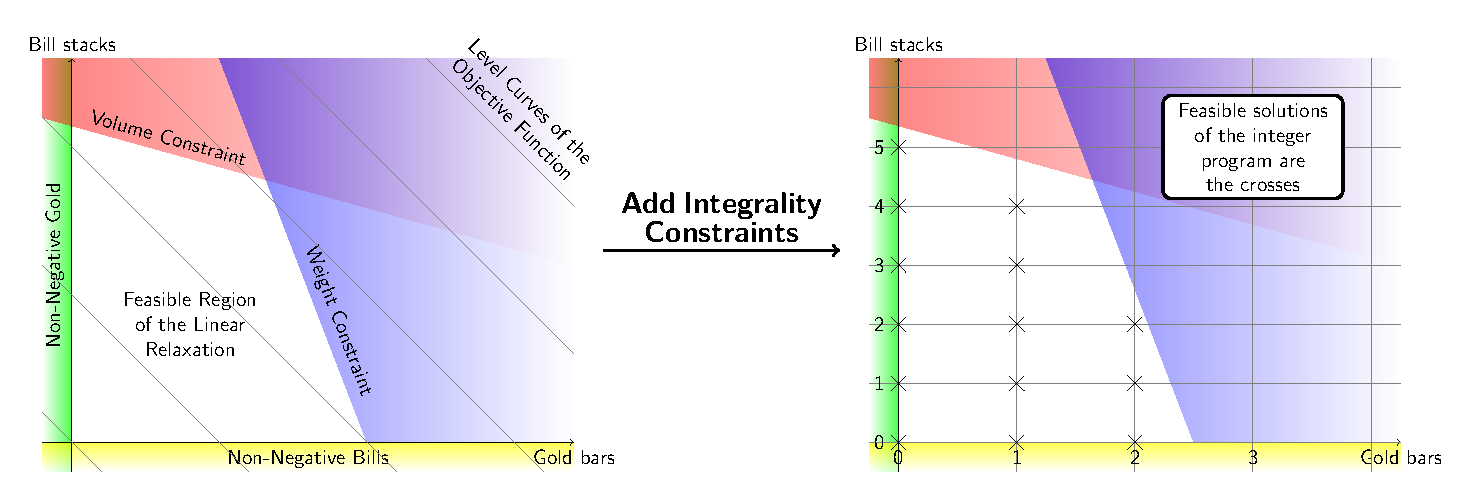
\includegraphics[width=\linewidth]{ILP.pdf}

    \href{http://www.science4all.org/article/integer-programming/}{from Lê Nguyên Hoang's http://www.science4all.org}
  \end{center}

\section{Graphical solution}

  \begin{itemize}
    \item Remember: An optimal feasible solution is a point in the feasible space that is as effective as any other point in achieving the specified goal.
    \item The solution of linear programming problems with only two decision variables can be illustrated graphically.
    \item If an optimal feasible solution exists, it occurs at one of the extreme points of the feasible space.
    \item We illustrate this for problems with one, with multiple, and with none optimal feasible solutions.
  \end{itemize}

  \begin{Exercise}
    \begin{equation*}
      \begin{aligned}
        \text{maximize } \quad & z = 3x_1 + x_2 \\
        \text{subject to }\quad &
        \begin{array}{rcl}
          x_2 & \leq & 5\\
          x_1 + x_2 &\leq& 10\\
          -x_1+x_2 &\geq& -2\\
          x_1,x_2 &\geq &0
        \end{array}
      \end{aligned}
    \end{equation*}
  \end{Exercise}
  \begin{center}
    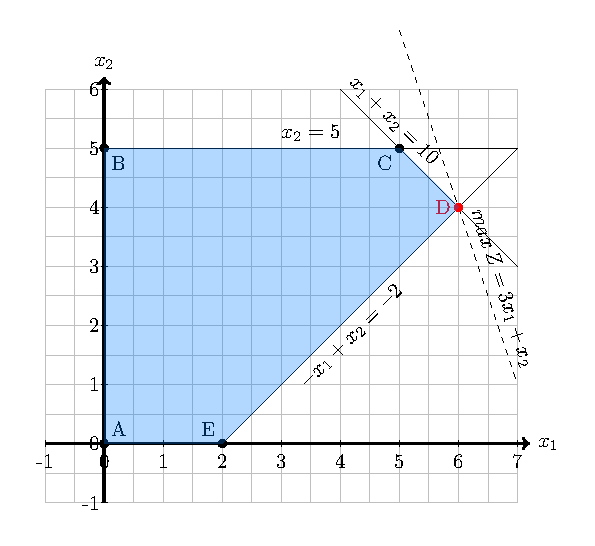
\includegraphics[width=0.6\linewidth]{LP2.pdf}
  \end{center}
  \begin{Exercise}
    \begin{equation*}
      \begin{aligned}
        \text{minimize } \quad & z = x_1 + x_2 \\
        \text{subject to }\quad &
        \begin{array}{rcl}
          3x_1 + x_2 & \geq & 6\\
          x_2 &\geq& 3\\
          x_1 &\leq& 4\\
          x_1,x_2 &\geq &0
        \end{array}
      \end{aligned}
    \end{equation*}
  \end{Exercise}

  \begin{center}
    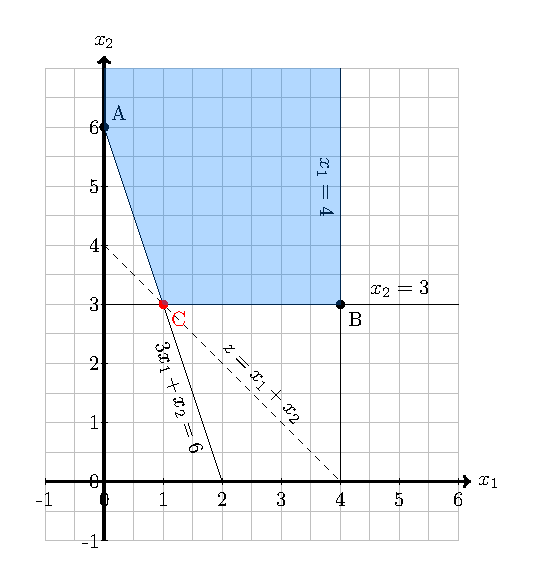
\includegraphics[width=0.6\linewidth]{LP6.pdf}
  \end{center}


  \begin{Exercise}
    \begin{equation*}
      \begin{aligned}
        \text{maximize } \quad & z = x_1 + 2x_2 \\
        \text{subject to }\quad &
        \begin{array}{rcl}
          -x_1+x_2 & \leq & 2\\
          x_1 + 2x_2 &\leq& 8\\
          x_1 &\leq& 6\\
          x_1,x_2 &\geq &0
        \end{array}
      \end{aligned}
    \end{equation*}
  \end{Exercise}
  %
  \begin{center}
   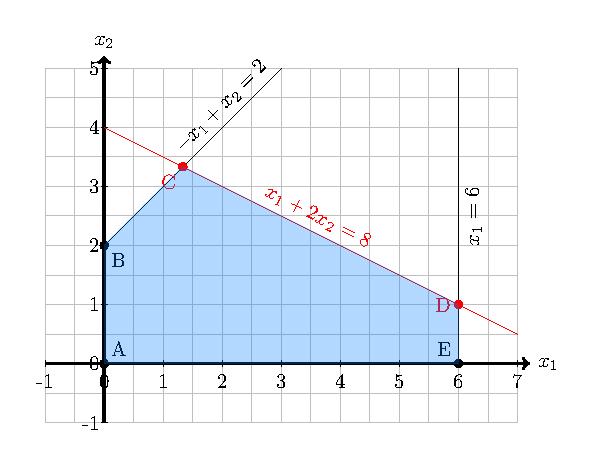
\includegraphics[width=0.7\linewidth]{LP3.pdf}
  \end{center}


  \begin{Exercise}
    \begin{equation*}
      \begin{aligned}
        \text{maximize } \quad & z = 3x_1 + x_2 \\
        \text{subject to }\quad &
        \begin{array}{rcl}
          x_1+x_2 & \geq & 4\\
          -x_1 + x_2 &\leq& 4\\
          -x_1 +2x_2 &\geq& -4\\
          x_1,x_2 &\geq &0
        \end{array}
      \end{aligned}
    \end{equation*}
  \end{Exercise}
  \begin{center}
   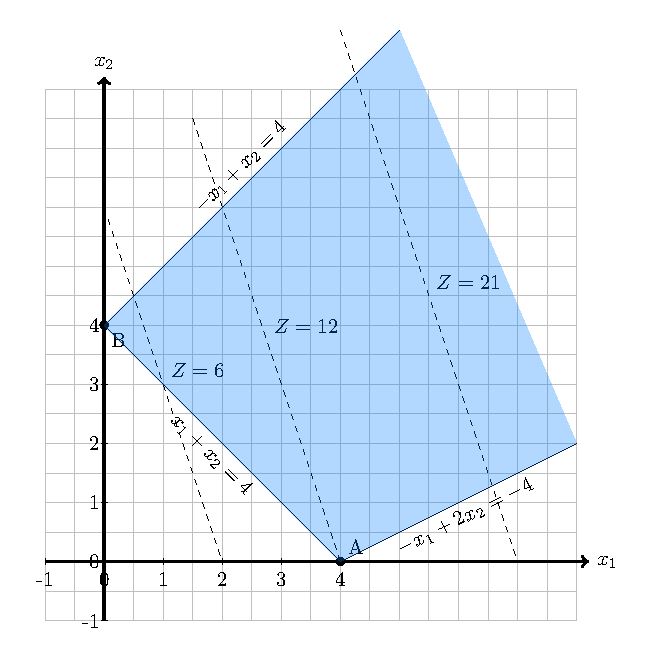
\includegraphics[width=0.7\linewidth]{LP4.pdf}
  \end{center}


  \begin{Exercise}
    \begin{equation*}
      \begin{aligned}
        \text{maximize } \quad & z = 3x_1 + x_2 \\
        \text{subject to }\quad &
        \begin{array}{rcl}
          -x_1 + x_2 &\geq& 4\\
          -x_1 +2x_2 &\leq& -4\\
          x_1,x_2 &\geq &0
        \end{array}
      \end{aligned}
    \end{equation*}
  \end{Exercise}
  \begin{center}
    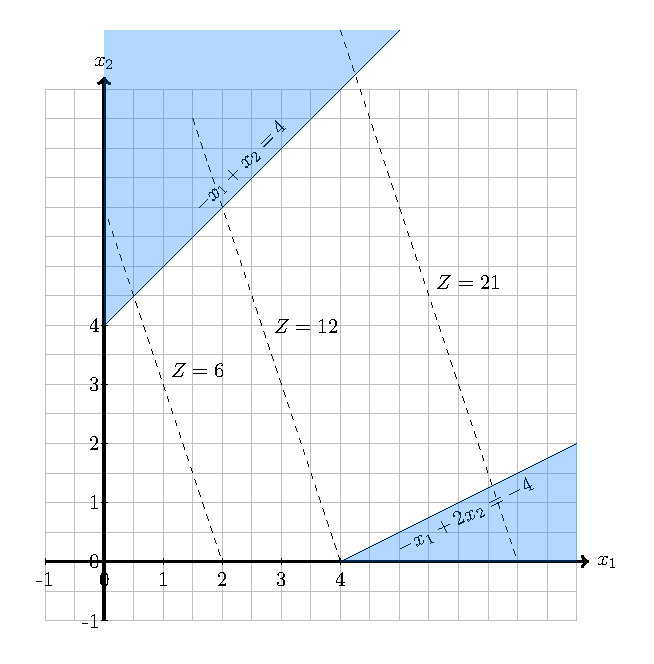
\includegraphics[width=0.7\linewidth]{LP5.pdf}
  \end{center}


\begin{program}
  E4. Build a Python code using Google OR tools' MPSolver interface to solve an arbitrary LP problem. Test it with the different exercises in this presentation.
\end{program}

\section{General solution method}

  \begin{itemize}
    \item If an optimal solution exists, it occurs at an extreme point of the feasible region.
    \item Only the finitely many extreme points need be examined (rather than all the points in the feasible region).
    \item Thus, an optimal solution may be found systematically by considering the objective function values at the extreme points.
    \item In fact, in actual practice, only a small subset of the extreme points need be examined.
  \end{itemize}
  This is the foundation for a {\bf general solution method} of a LP problem called the {\bf Simplex method}.

%----------------------------------------------------------------------------------------




\title[Introduction]{Unit 2. Linear programming. The Simplex Method}



%%%%%%%%%%%%%%%%%%%%%%%%%%%%%%%%%%%%%%%%%%%%%%%%%%%%%%%%%%%%%%%%%%%%%%%%%%%%%
%%%%%%%%%%%%%%%%%%%%%%%%%%%%%%%%%%%%%%%%%%%%%%%%%%%%%%%%%%%%%%%%%%%%%%%%%%%%%
%%%%%%%%%%%%%%%%%%%%%%%%%%%%%%%%%%%%%%%%%%%%%%%%%%%%%%%%%%%%%%%%%%%%%%%%%%%%%

\begin{itemize}
  \item Understanding the rational behind the Simplex method for LP.
  \item Understanding and practicing the algorithm in 2 variables.
  \item Recognizing the different types of results one can achieve in LP from the Simplex Method algorithm.
  \item Getting familiar with slack, surplus and artificial variables.
\end{itemize}

\section{Introduction to the Simplex method for LP}

  \begin{center}
    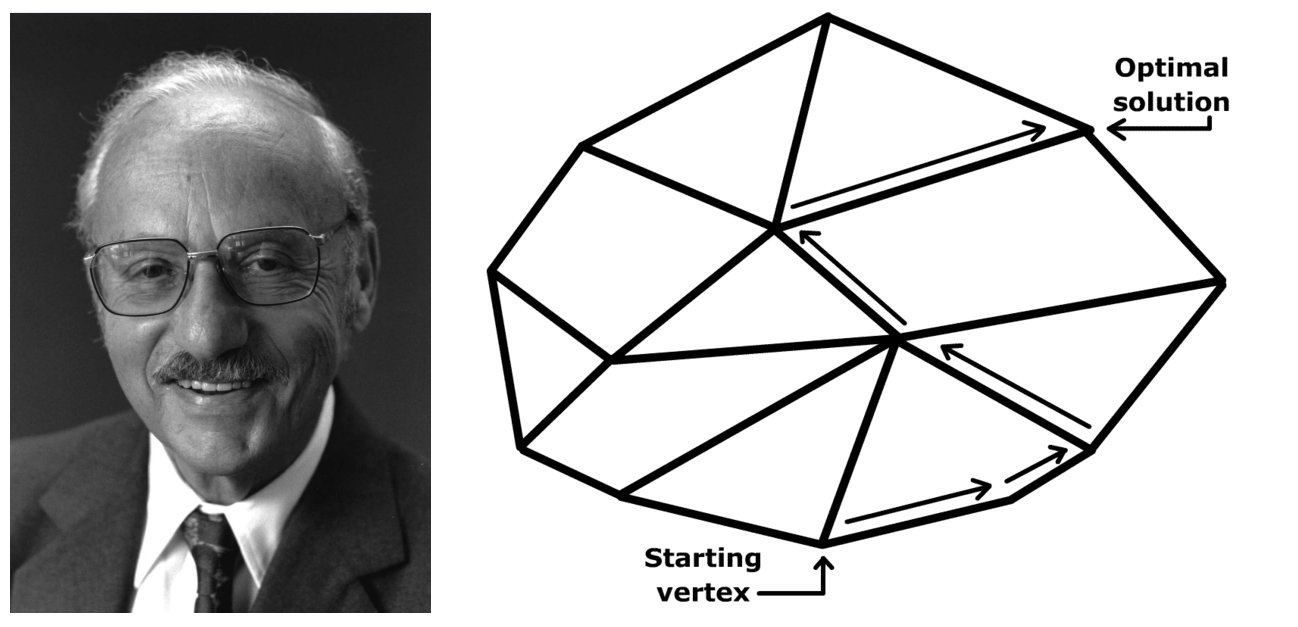
\includegraphics[width=\linewidth]{george-danzig-simplex.jpg}
  \end{center}

  Left: George Dantzig (1914-2005), the American mathematical scientist who devised linear programming and the simplex algorithm. Right: The simplex algorithm moves along the edges of the polytope until it reaches the optimum solution [Image Wikimedia Commons].

\section{Preparing the LP problem for applying the Simplex method}

 
      \begin{center}
        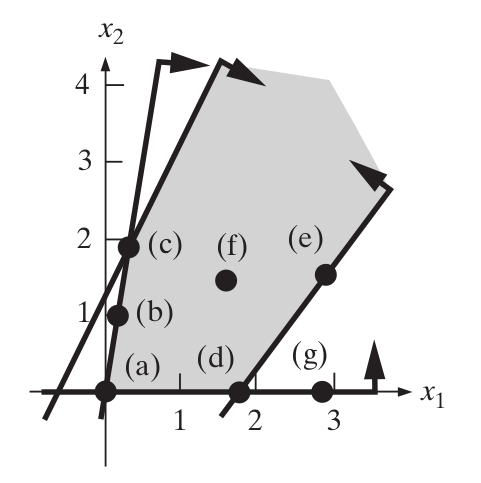
\includegraphics[width=\linewidth]{points_classification.png}
      \end{center}
   
      (a), (c), and (d) are both extreme points and boundary points. \\
      (b) and (e) are boundary points that are not extreme. \\
      (f) is interior because no constraint is active. \\
      (g) is neither interior nor boundary (nor extreme) because it is infeasible.\cite{rardin}




  \begin{minipage}{7cm}{Standard form}
    For a LP with $n$ variables and $m$ constraints, the standard form is given by:
    \begin{equation*}
      \begin{aligned}
        \text{maximize } \quad & z = c_1x_1+c_2x_2 +\cdots + c_nx_n \\
        \text{subject to }\quad &
        \begin{array}{rcl}
          a_{11}x_1+a_{12}x_2+\cdots+a_{1n}x_n &= &b_1 \\
          a_{21}x_1+a_{22}x_2+\cdots+a_{2n}x_n &= &b_2 \\
          \vdots &=& \vdots\\
          a_{m1}x_1+a_{m2}x_2+\cdots+a_{mn}x_n &= &b_m \\
        \end{array}
      \end{aligned}
    \end{equation*}
    where $x_1,\ldots,x_n\geq0$ and $b_1,\ldots,b_m\geq0$
  \end{minipage}

Thus:
\begin{equation*}
  \begin{aligned}
    \text{maximize } \quad & z = cx \\
    \text{subject to }\quad &
    \begin{array}{c}
      Ax=b\\
      x\geq0\\
      b\geq0
    \end{array}
  \end{aligned}
\end{equation*}


Of course, not always the system is proposed in this standard form, so\cite{carter}:
\begin{itemize}
  \item We need to leave a maximization problem. If the problem is to minimize the objective function, we simply multiply it by $(-1)$.
  \item In order to change inequality constraints into equality constraints we use {\it slack} variables for $\leq$ inequalities:
  \[
  3x_1+4x_2 \leq 7  \rightarrow  3x_1+4x_2+s_1 =7
  \]
  or {\it surplus} variables for $\geq$ inequalities:
  \[
  x_1+3x_2\geq 10 \rightarrow x_1+3x_2 -s_2 =10
  \]
  \item All variables should be non-negative. If some variable $x_1$ needs to be considered as unrestricted in sign, we will replace it by $x_1'-x_1''$, with $x_1',x_1''\geq 0$
\end{itemize}

\section{The algebra behind the standard form}

  \begin{itemize}
 \item The system of linear equations, $Ax = b$, consists of $m$ equations and $n$
unknowns (the original decision variables plus the rest introduced to get a standard form). If the system has any solution, then $m \leq n$.
\item If $m = n$ (and if $rank (A) = m$ and $A$ is nonsingular), then 
$x = A^{-1}b$. No optimization needed!
\item If $m < n$, there are infinitely many solutions and $n -m$ degrees of freedom. 
\item A {\bf basic solution} is obtained by setting $n - m$ of the variables to zero ({\bf non-basic variables}), and solving for the remaining ({\bf basic}) $m$ variables. The number of basic solutions is $\binom{n}{n-m}=\binom{n}{m}=\frac{n!}{m!(n-m)!}$
\item Basic solutions that do not satisfy all problem constraints and non-negativity constraints are {\bf infeasible solutions}.
\item An {\bf optimal basic feasible solution} is a
basic feasible solution that optimizes the objective function. 
\end{itemize}

\section{The Simplex algorithm}

We define
two extreme points of the feasible region (or two basic feasible solutions) as being adjacent if all but one of their basic variables are the same. Thus, {\em a transition from one basic
feasible solution to an adjacent basic feasible solution can be thought of as exchanging
the roles of one basic variable and one non-basic variable}. The Simplex method performs a sequence of such transitions and thereby examines a succession of adjacent
extreme points. A transition to an adjacent extreme point will be made only if by doing
so the objective function is improved (or stays the same). It is a property of linear programming problems that this type of search will lead us to the discovery of an optimal
solution (if one exists). The Simplex method is not only successful in this sense, but it
is remarkably efficient because it succeeds after examining only a fraction of the basic
feasible solutions.\cite{carter}

The algorithm consists in:
\begin{enumerate}
  \item obtaining an initial feasible
solution,
\item make transitions to a better basic feasible solution,
\item recognizing an optimal solution.
\end{enumerate}
From any basic feasible solution, we have the assurance
that, if a better solution exists at all, then there is an adjacent solution that is better than the
current one.\cite{carter}

\begin{enumerate}
  \item Convert the system of inequalities to equations (using slack or surplus variables).
  \item Set the objective function to zero.
  \item Create the Simplex tableau and label active and basic variables.
  \item Select the pivot column (the one with the most negative coefficient in the zeroed objective function). Linked to the {\bf entering variable}.
  \item Select the pivot row (once divided the entry in the constant column by the ceffient in that row in the pivot column, we choose the smallest ratio). Linked to the {\bf leaving variable}.
  \item The pivot is the intersection between the pivot row and pivot column.
  \item Use the pivot value to make zeros in the rest of elements in the column.
  \item Repeat the process from step 4, until the last row is all non-negative.
\end{enumerate}




  \begin{equation*}
    \begin{aligned}
      \text{maximize } \quad & z = 8x_1+5x_2 \\
      \text{subject to }\quad &
      \begin{array}{rcl}
        x_1 &\leq &150 \\
        x_2 &\leq &250 \\
        2x_1+x_2 &\leq &500 \\
        x_1,x_2 &\geq& 0
      \end{array}
    \end{aligned}
  \end{equation*}
We build first the standard form:
\begin{eqnarray*}
  -8x_1-5x_2-0s-0t-0u+z&=&0\\
  x_1+s&=&150\\
  x_2+t&=&250\\
  2x_1+x_2+u&=&500
\end{eqnarray*}

  We write the coefficients matrix and we identify the basic ($m=3$) and non-basic ($n-m=5-3=2$ degrees of freedom) variables:
  \begin{equation}
\begin{array}{cc}
&\\
&z \\
\rightarrow &s \\
&t \\
&u\\
\mathrm{basic}
\end{array}
%
\begin{array}{c|ccccc|c}
  z & x_1 & x_2 & s & t & u & b \\ \hline
  1 & -8 & -5 & 0 & 0 & 0 & 0 \\ \hline
  0 & 1 & 0 & 1 & 0 & 0 & 150  \\
  0 & 0 & 1 & 0 & 1 & 0 & 250 \\
  0 & 2 & 1 & 0 & 0 & 1 & 500 \\
    & \uparrow & & & & &
\end{array}
%\end{matrix}
\end{equation}
  Note that the basic variables are those for which each column is a collection of 1 and zero. We will arbitrarily assign zeros to the non-basic variables.
So a possible solution is $\boxed{P_A=(x_1=0, x_2=0)\Rightarrow z=0}$.

  The arrow marks the pivot column. We will take the pivot row by considering which is the lowest value among 150/1 and 500/2. So, the pivot row corresponds to the $s$ basic variable.

%   \begin{center}
%    \includegraphics[width=0.5\linewidth]{LP7.pdf}
%   \end{center}


\begin{equation*}
\begin{array}{cc}
&\\
R_1+8R_2&z \\
&x_1 \\
&t \\
\rightarrow R_4-2R_2&u\\
&\mathrm{basic} \\
\end{array}
\begin{array}{c|ccccc|c}
  z & x_1 & x_2 & s & t & u & b \\ \hline
  1 & 0 & -5 & 8 & 0 & 0 & 1200 \\ \hline
  0 & 1 & 0 & 1 & 0 & 0 & 150  \\
  0 & 0 & 1 & 0 & 1 & 0 & 250 \\
  0 & 0 & 1 & -2 & 0 & 1 & 200 \\
    &  & \uparrow& & & &
\end{array}
\end{equation*}
$P_B=(150,0)$ and $z(P_B)=1200$ with $t=250$, $u=200$, $s=0$.

\begin{equation*}
\begin{array}{cc}
&\\
R_1+5R_4&z \\
&x_1 \\
\rightarrow R_3-R_4&t \\
&x_2\\
&\mathrm{basic} \\
\end{array}
\begin{array}{c|ccccc|c}
  z & x_1 & x_2 & s & t & u & b \\ \hline
  1 & 0 & 0 & -2 & 0 & 5 & 2200 \\ \hline
  0 & 1 & 0 & 1 & 0 & -1 & 150  \\
  0 & 0 & 0 & 2 & 0 & 1 & 50 \\
  0 & 0 & 1 & -2 & 0 & 1 & 200 \\
    &  & & \uparrow& & &
\end{array}
\end{equation*}

\begin{equation*}
\begin{array}{cc}
&\\
R_1+5R_4&z \\
&x_1 \\
\rightarrow R_3-R_4&s \\
&x_2\\
&\mathrm{basic} \\
\end{array}
\begin{array}{c|ccccc|c}
  z & x_1 & x_2 & s & t & u & b \\ \hline
  1 & 0 & 0 & 0 & 1 & 4 & 2250 \\ \hline
  0 & 1 & 0 & 0 & -1/2 & 1/2 & 125  \\
  0 & 0 & 0 & 1 & 1/2 & -1/2 & 25 \\
  0 & 1 & 0 & 1 & 0 & 0 & 250 \\
    &  & & \uparrow& & &
\end{array}
\end{equation*}

$\boxed{P_D=(125,250)}$ and $\boxed{z(P_D)=2250}$ with $t,u=0$ (binding constraints), $s=25$ (non-binding constraint).


  \begin{center}
    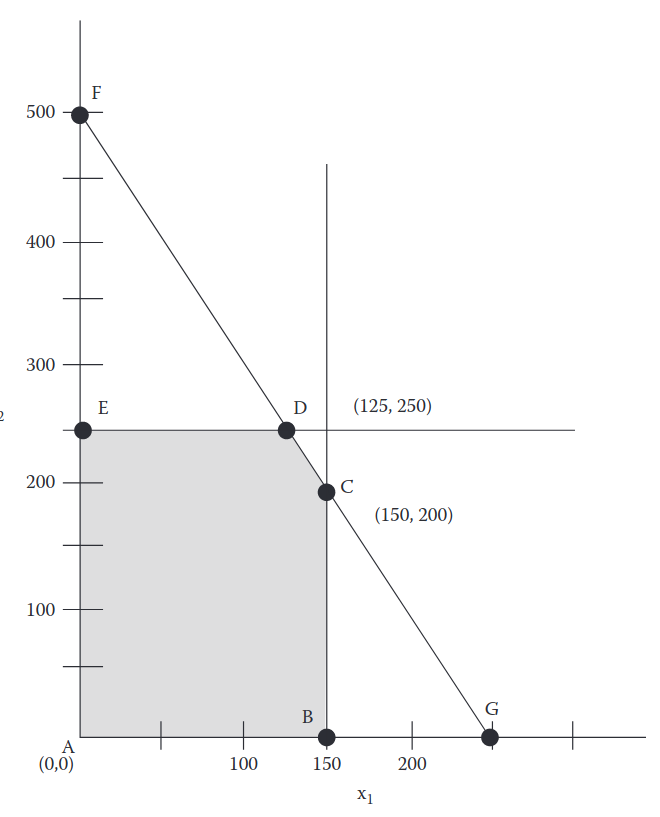
\includegraphics[width=0.4\linewidth]{simplex_example.png}
  \end{center}
  Simplex steps for the given example (taken from \cite{carter}).

  Solve, using the Simplex method, the Exercises 3 through 6 of the previous session.

\section{Initial solutions for General Constraints}


  When adding slack variables, we end up finding an initial feasible set of basic variables. But what happens when not all constraints are of the form "$\leq$"?\cite{carter}

  \begin{enumerate}
    \item Make all right hand sides $b_i$ of the constraint (in)equalities positive. If they are not, multiply the expression by $(-1)$.
    \item If we end up just with slack variables, they can be directly used as initial basic variables. If the expressions are of the type $\geq$ the selection of initial basic variables is not trivial.
    \item We then create {\bf artificial variables}, as a trick to create a starting basic solution
  \end{enumerate}
  \begin{equation*}
    \begin{aligned}
      \text{maximize } \quad & z = x_1+3x_2 \\
      \text{subject to }\quad &
      \begin{array}{rcl}
        2x_1 -x_2 &\leq &-1 \\
        x_1+x_2 &= &3 \\
        x_1,x_2 &\geq& 0
      \end{array}
    \end{aligned}
  \end{equation*}

  By leaving the right hand side of the constraints positive and adding a surplus variable, we end up having
  \begin{equation*}
    \begin{aligned}
       \text{subject to }\quad &
      \begin{array}{rcl}
        -2x_1 +x_2 -s_1 &= &1 \\
        x_1+x_2 &= &3
      \end{array}
    \end{aligned}
  \end{equation*}
  and now we introduce the artificial variables to create an initial solution:
  \begin{equation*}
    \begin{aligned}
       \text{subject to }\quad &
      \begin{array}{rcl}
        -2x_1 +x_2 -s_1 +R_1&= &1 \\
        x_1+x_2 +R_2&= &3
      \end{array}
    \end{aligned}
  \end{equation*}
  with all variables non-negative. Recall that, in fact, $R_1=R_2=0$, so they will be just used temporarily.
  \\[10pt]

  There are two main methods to solve the problem: the two-phase method, explained next, and the \href{https://www.youtube.com/watch?v=btjxqq-vMOg}{big-M method}, that we are not explaining here.


  \begin{enumerate}
    \item First we will use the Simplex method to minimize the values of $R_1$ and $R_2$. 
    \item If they reach the value of zero, there is a solution for the original problem. If not, there is no feasible solution to the original problem.
  \end{enumerate}
  In the above example, we want to minimize the function $z_R=R_1+R_2$ or, what is the same, we want to maximize the function $z_R=-R_1-R_2$
  \begin{equation*}
    \begin{array}{c}
    \\
    z_R\\
    R_1\\
    R_2\\
    \end{array}
    \begin{array}{ccccc|c}
       x_1 & x_2 & s_1 & R_1 & R_2 & Solution \\ \hline
       0 & 0 & 0 & 1 & 1 & 0 \\ \hline
       -2 & 1 & -1 & 1 & 0 & 1  \\
       1 & 1 & 0 & 0 & 1 & 3 \\
    \end{array}
    \end{equation*}

  Next, we transform the problem in order to get  basic variables (columns of one 1 and the rest zeros). For example, by using the second and third row to make appear 0 in the first row for the artificial variables:
  \begin{equation*}
    \begin{array}{c}
    \\
    z_R\\
    R_1\\
    R_2\\
    \end{array}
    \begin{array}{ccccc|c}
       x_1 & x_2 & s_1 & R_1 & R_2 & Solution \\ \hline
       1 & -2 & 1 & 0 & 0 & -4 \\ \hline
       -2 & 1 & -1 & 1 & 0 & 1  \\
       1 & 1 & 0 & 0 & 1 & 3 \\
    \end{array}
  \end{equation*}
  We can solve this problem with the Simplex method, obtaining a tableau:
  \begin{equation*}
    \begin{array}{c}
    \\
    z_R\\
    x_2\\
    x_1\\
    \end{array}
    \begin{array}{ccccc|c}
       x_1 & x_2 & s_1 & R_1 & R_2 & Solution \\ \hline
       0 & 0 & 0 & 1 & 1 & 0 \\ \hline
       0 & 1 & -1/3 & 1/3 & 2/3 & 7/3  \\
       1 & 0 & 1/3 & -1/3 & 1/3 & 2/3 \\
    \end{array}
  \end{equation*}
    which provides the optimal solution for Phase 1. This means that the original problem has solution (as $R_1=R_2=0$). In Phase 2, we will replace the first row by the original maximization problem and leave out the artificial variables, solving the now standard Simplex problem:
    \begin{equation*}
      \begin{array}{c}
        \\
        z\\
        x_2\\
        x_1\\
      \end{array}
      \begin{array}{ccc|c}
        x_1 & x_2 & s_1 &  Solution \\ \hline
        -1 & -3 & 0 &  0 \\ \hline
        0 & 1 & -1/3 & 7/3  \\
        1 & 0 & 1/3  & 2/3 \\
      \end{array}
    \end{equation*}
    that leads to
    \begin{equation*}
      \begin{array}{c}
        \\
        z\\
        x_2\\
        s_1\\
      \end{array}
      \begin{array}{ccc|c}
        x_1 & x_2 & s_1 &  Solution \\ \hline
        2 & 0 & 0 &  9 \\ \hline
        1 & 1 & 0 & 3  \\
        3 & 0 & 1  & 2 \\
      \end{array}
    \end{equation*}

      Draw the graphical solution of this problem and interpret the results.


    Some special cases:
    \begin{description}
      \item[Multiple optimal solutions] If a zero appears in the objective function row corresponding to a non-basic
      variable, then that non-basic variable can enter the basis without changing the value of
      the objective function. So, two adjacent points have the same objective function value.
      \item[Unbounded solution] If in any tableau the constraint coefficients corresponding to a non-basic variable are all
      either negative or zero, then that non-basic variable can be increased arbitrarily without
      violating any constraint. Thus, the feasible region is unbounded in the direction of that
      variable.
      \item[Degenerate solutions] A solution to a linear programming problem is said to be degenerate if one or more of the
      basic variables has a value of zero. This shows redundancy in the constraints.
    \end{description}

\section{Application of SIMPLEX to non-linear problems}


  Algorithm (see example in the next page):
\begin{enumerate}
\item In $\mathbf{R}^2$, we form a triangle with vertices at $x^{[0]}$ and the two points $x^{[1]} = x^{[0]} + l_1e^{[1]}$ and  $x^{[2]} = x^{[0]} + l_2e^{[2]}$. In $\mathbf{R}^N$ the triangle becomes a simplex with $N + 1$ vertices.
\item We aim at moving ${x^{[0]}, x^{[1]}, x^{[2]},...}$ so that the triangle comes to enclose a local minimum $x_{\mathrm{min}}$ while shrinking in size.  First, the vertex of highest cost function value is moved in the direction of the {\bf triangle’s center} towards a region where we expect the cost function values to be lower. After a sequence of such moves, the triangle eventually contains in its interior a local minimum. 
\item The size of the triangle is progressively reduced until it tightly bounds the local minimum, as the vertex moves are most likely to succeed when the triangle is small enough that $F(x)$ varies linearly over the triangle region.
\end{enumerate}

  \begin{center}
    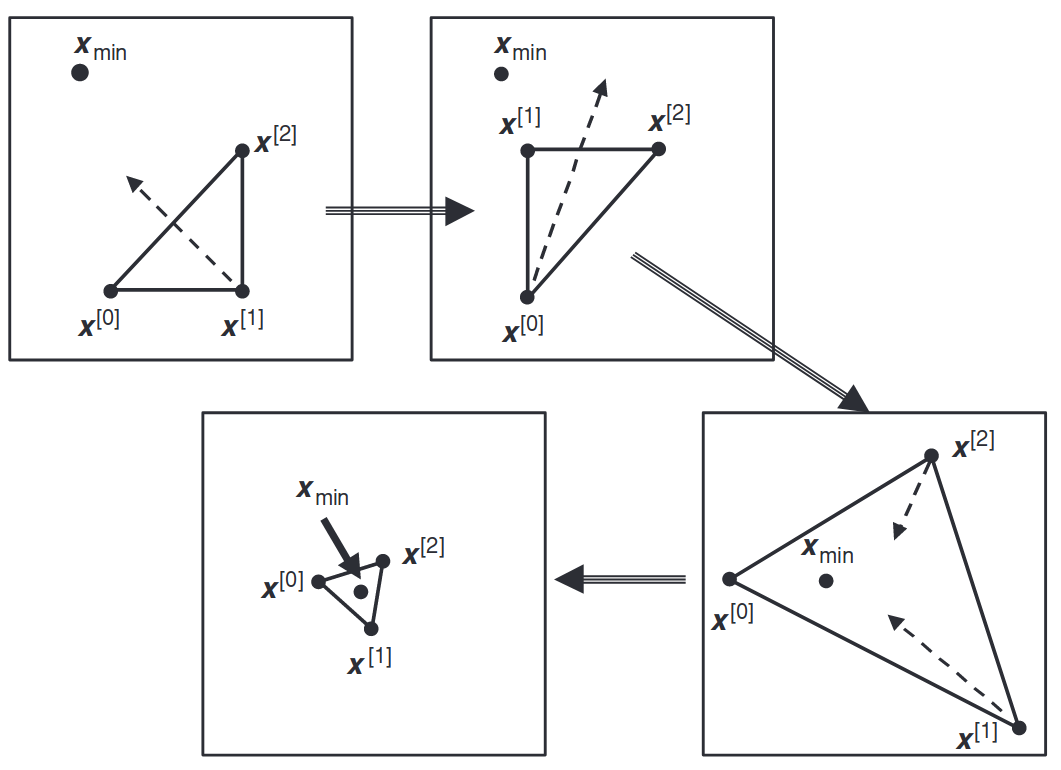
\includegraphics[width=0.7\linewidth]{simplex_nonlinear.png}
  \end{center}
  The simplex method moves the vertices of the simplex (in two dimensions, a triangle) until it contains the local minimum, and shrinks the simplex to find the local minimum (taken from \cite{beers}).

%----------------------------------------------------------------------------------------




\title[Introduction]{Unit 2. Linear programming. Duality}



%%%%%%%%%%%%%%%%%%%%%%%%%%%%%%%%%%%%%%%%%%%%%%%%%%%%%%%%%%%%%%%%%%%%%%%%%%%%%
%%%%%%%%%%%%%%%%%%%%%%%%%%%%%%%%%%%%%%%%%%%%%%%%%%%%%%%%%%%%%%%%%%%%%%%%%%%%%
%%%%%%%%%%%%%%%%%%%%%%%%%%%%%%%%%%%%%%%%%%%%%%%%%%%%%%%%%%%%%%%%%%%%%%%%%%%%%

\begin{itemize}
  \item Understanding Dual and Primal problems in LP
  \item Economic interpretation
  \item Conditions of optimality
  \item Resolution of the dual by the primal and penalty method
\end{itemize}

\section{Duality}
\note{\url{https://www.youtube.com/watch?v=yU8updOR87c}}

  Linear programming problems come in pairs!

  \begin{equation*}
    \begin{aligned}
      \text{maximize  } \quad & 4x_1 + x_2 +5x_3 +3x_4 \\
      \text{subject to }\quad &
      \left\{
      \begin{array}{rcl}
        x_1 - x_2 -x_3 +3x_4 &\leq &1 \\
        5x_1 + x_2 +3x_3 +8x_4 &\leq &55 \\
        -x_1 + x_2 +3x_3 -5x_4 &\leq &3 \\
        x_1,x_2,x_3 &\geq& 0
      \end{array}
      \right.
    \end{aligned}
  \end{equation*}

note that
\begin{eqnarray*}
  y_1(x_1 - x_2 -x_3 +3x_4)&+&\\y_2(5x_1 + x_2 +3x_3 +8x_4)&+&\\y_3(-x_1 + x_2 +3x_3 -5x_4) &\leq& y_1+55y_2+3y_3
\end{eqnarray*}


We see that maximizing the {\bf Primal objective function} $4x_1 + x_2 +5x_3 +3x_4$ is
  equivalent to minimize the {\bf Dual objective function} $y_1+55y_2+3y_3$:

    \begin{equation*}
    \begin{aligned}
      \text{minimize } \quad & y_1+55y_2+3y_3 \\
      \text{subject to }\quad &
      \left\{
      \begin{array}{rcl}
        y_1 + 5y_2 -y_3 &\geq &4 \\
        -y_1 +y_2 +y_3 &\geq &1 \\
        -y_1 +3y_2 +3y_3 &\geq &5 \\
        3y_1 +8y_2 -5y_3 &\geq &3 \\
        y_1,y_2,y_3,y_4 &\geq& 0
      \end{array}
      \right.
    \end{aligned}
  \end{equation*}



In general, if we can write the LP problem in its {\bf normal formulation}:
\[
\begin{rcases}
\text{min }\quad\uvec{c}^t \uvec{x}\\
\text{subject to }\quad A\uvec{x}\geq \uvec{b}, \forall x_i\geq0
\end{rcases} \text{PRIMAL}
\]

\[
\begin{rcases}
\text{max }\quad\uvec{b}^t \uvec{y}\\
\text{subject to }\quad A^t\uvec{y}\leq \uvec{c}, \forall y_i\geq0
\end{rcases} \text{DUAL}
\]
The dual problem is a transposition of the primal problem. Since any LP can be written in the standard form
above, any LP has a dual.

  \begin{enumerate}
    \item if you are asked to minimize $f(x)$, this is equivalent to maximize $-f(x)$;
    \item add slack/surplus variables if you want to transform an inequality into an equality contraint;
    \item $a\cdot x=b$ is equivalent to having, simultaneously, $a \cdot x \leq b$ and $a \cdot x \geq b$;
    \item replace an unconstrained variable $x_i$ by $u_i-v_i$ and impose that $u_i,v_i \geq 0$
  \end{enumerate}
  Trick: Leave equality constraints to use the simplex algorithm. Use the inequality constraints for the duality theorem to be used.

\begin{Exercise}
  Find the dual problem of
  \begin{equation*}
  \begin{aligned}
    \text{maximize } \quad & 3x_1 +2x_2 \\
    \text{subject to }\quad &
    \left\{
    \begin{array}{rcl}
      2x_1+x_2 &\leq &4 \\
      2x_1+3x_2 &\leq &6 \\
      x_1,x_2 &\geq& 0
    \end{array}
    \right.
  \end{aligned}
\end{equation*}
Solve it graphically and using Simplex. 
\end{Exercise}

\note{\begin{center}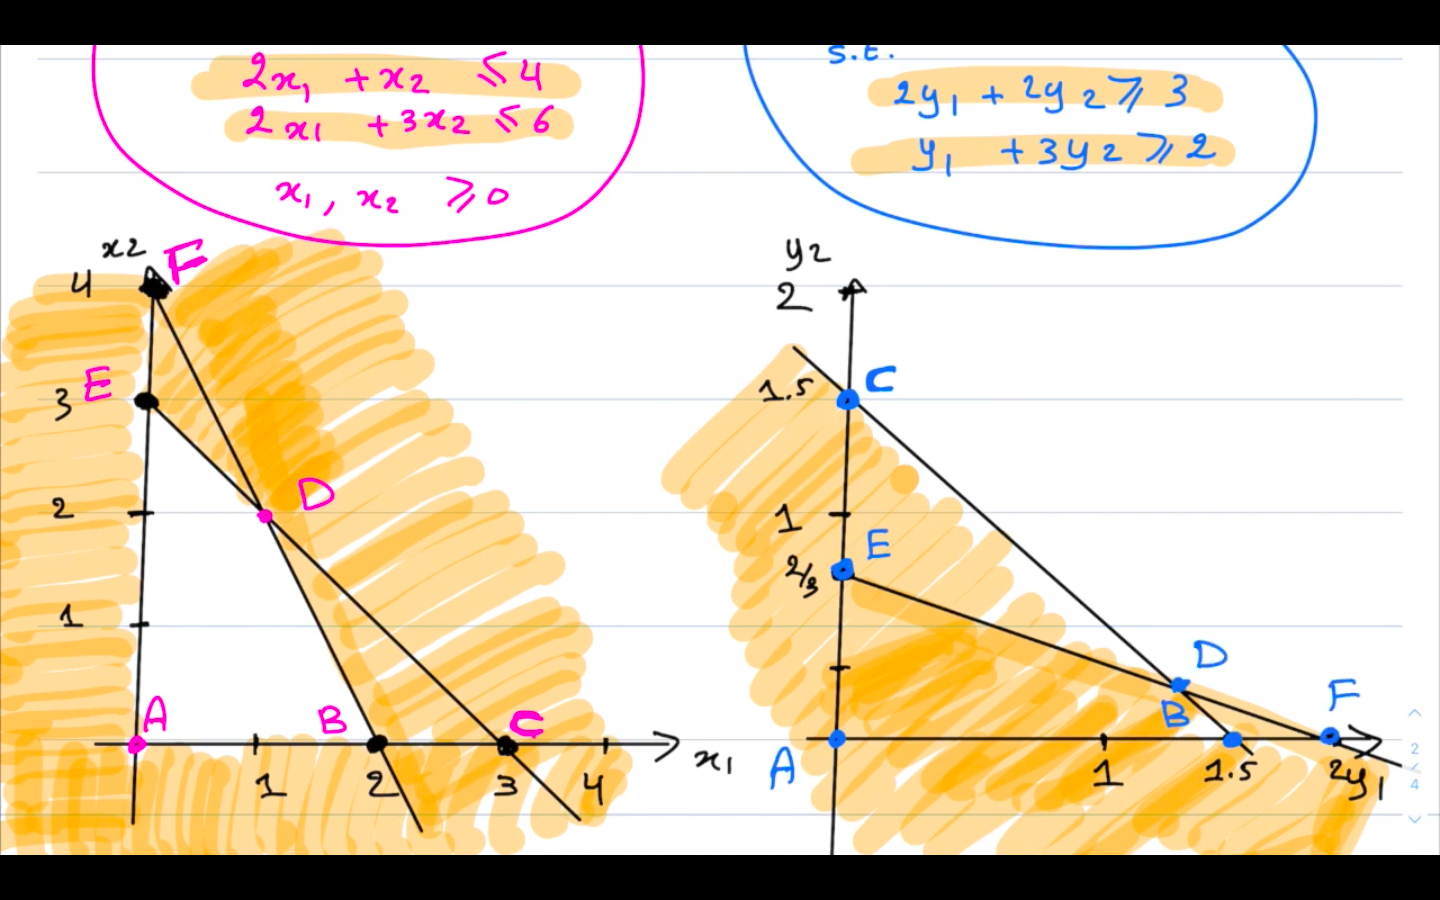
\includegraphics[width=0.8\linewidth]{answer1.png}\end{center}}
\note{\begin{center}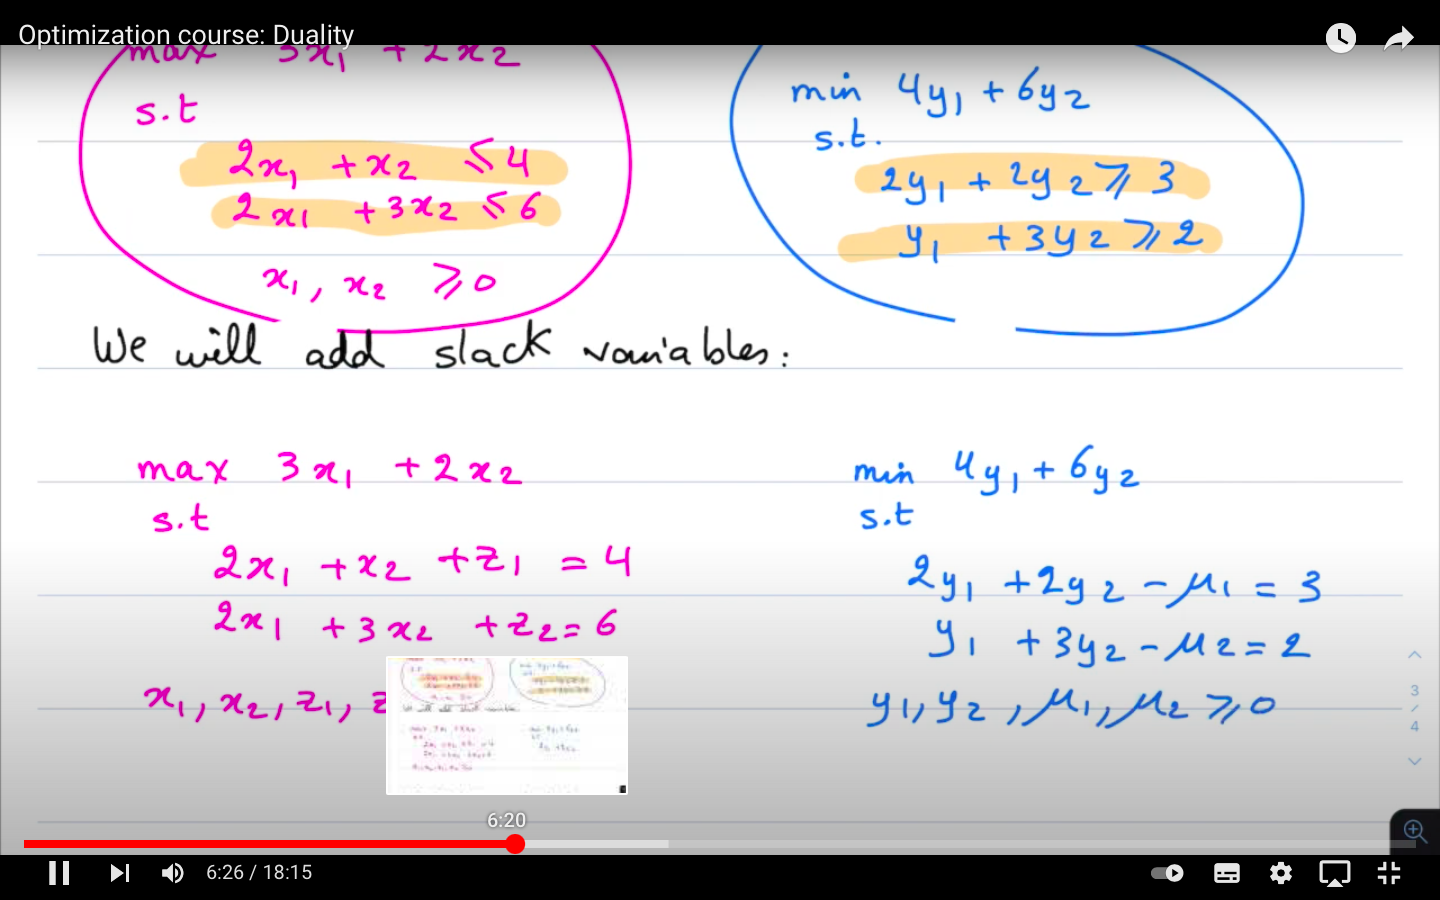
\includegraphics[width=0.8\linewidth]{answer3.png}\end{center}}
\note{\begin{center}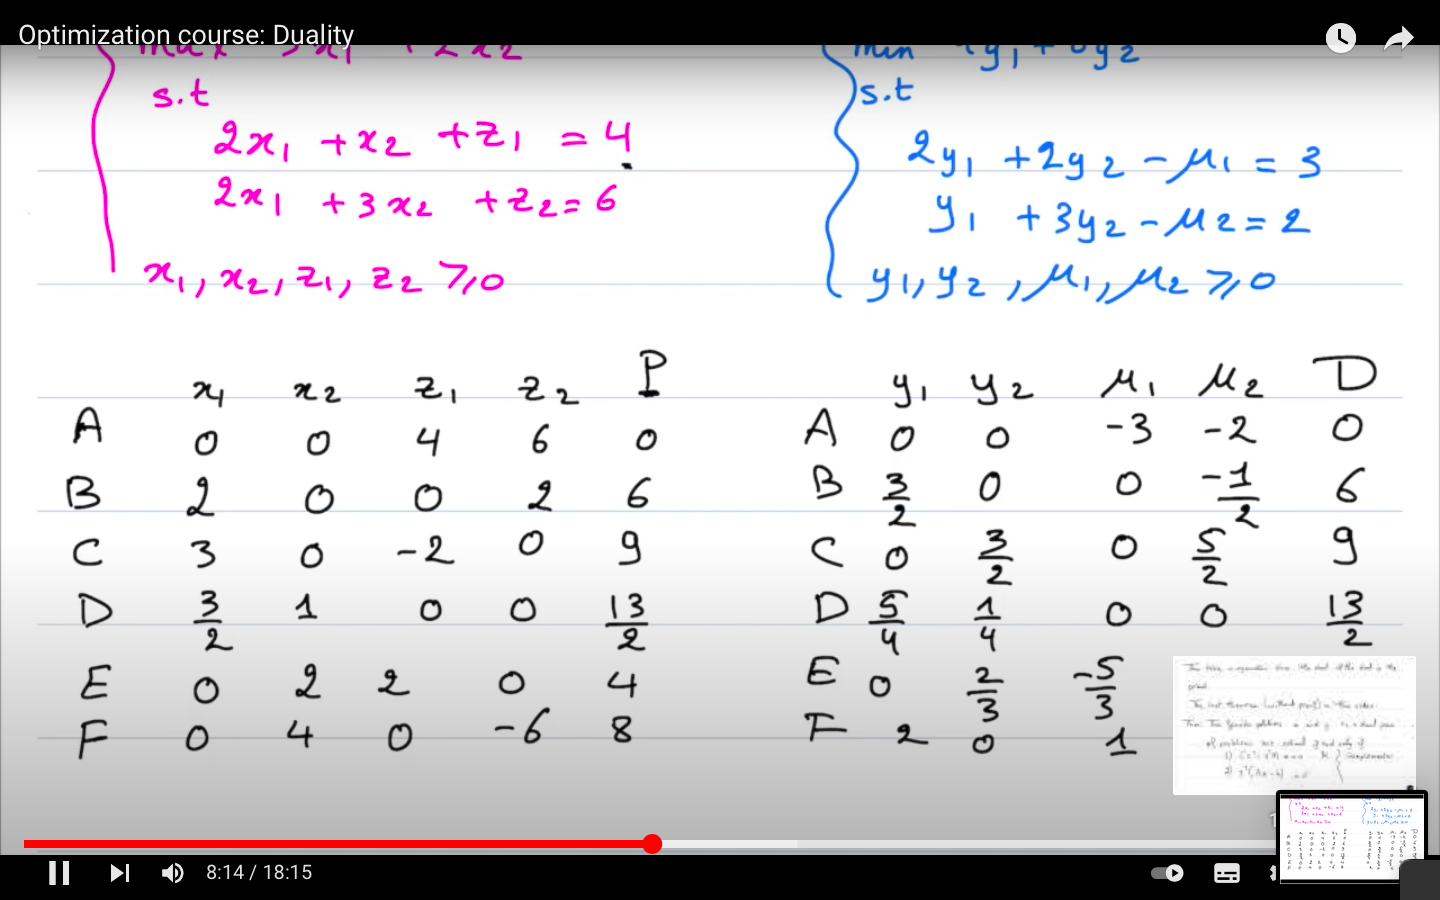
\includegraphics[width=0.8\linewidth]{answer2.png}\end{center}}
\note{\begin{center}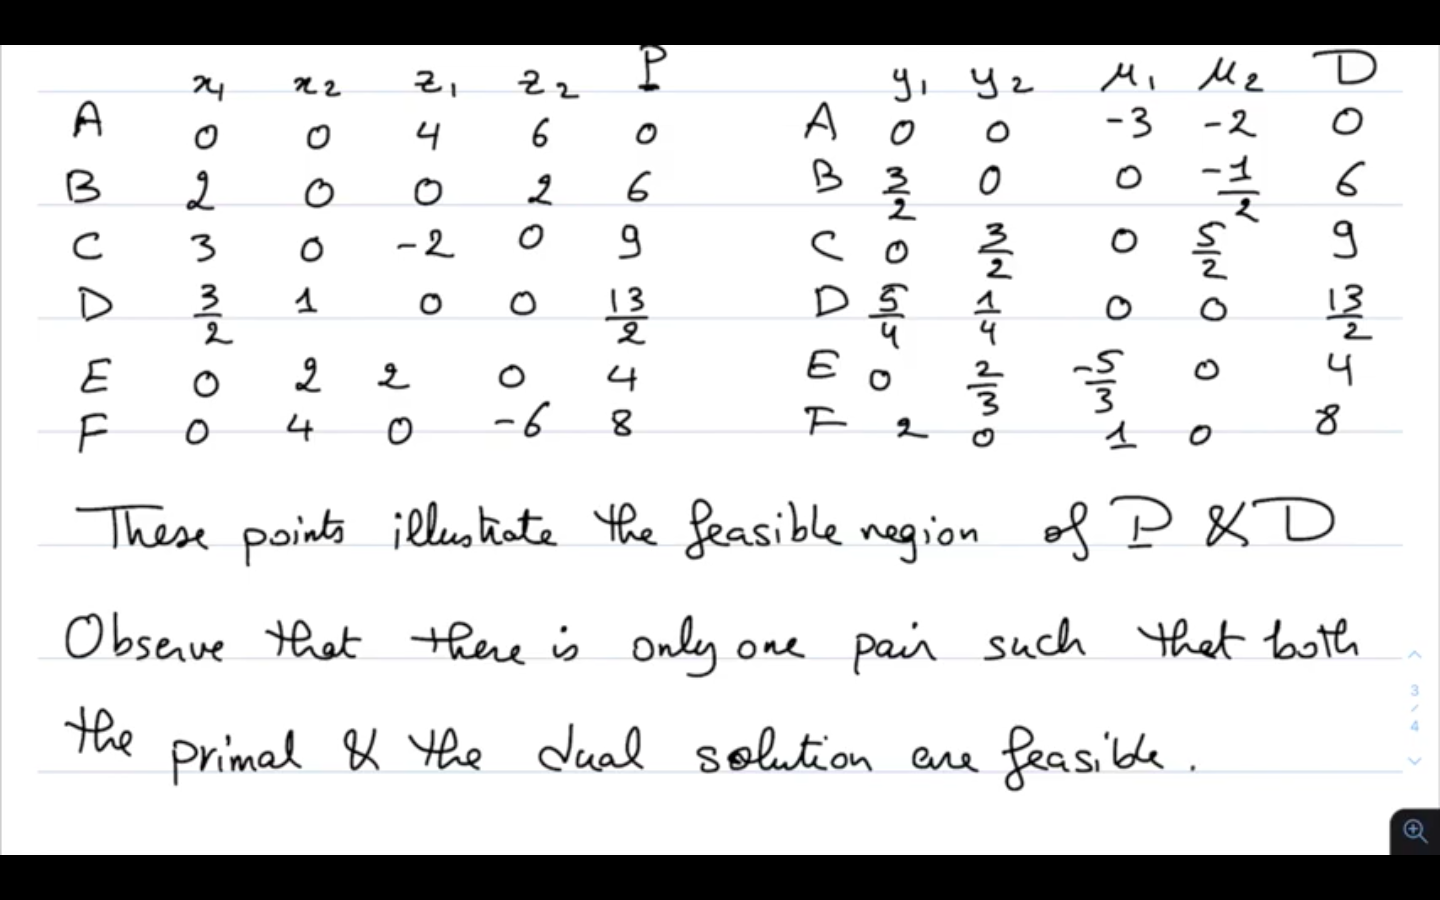
\includegraphics[width=0.8\linewidth]{answer4.png}\end{center}}

\begin{Exercise}
  Find the dual problem of
  \begin{equation*}
  \begin{aligned}
    \text{minimize } \quad & 4x_1 +4x_2+x_3 \\
    \text{subject to }\quad &
    \left\{
    \begin{array}{rcl}
      x_1+x_2+x_3 &\leq &2 \\
      2x_1+x_2 &= &3 \\
      2x_1+x_2+3x_3 &\geq &3 \\
      x_1,x_2,x_3 &\geq& 0
    \end{array}
    \right.
  \end{aligned}
\end{equation*}
Trick: normalize the problem first: eg $2x_1+x_2=3 \rightarrow \begin{cases}2x_1+x_2 \geq 3\\2x_1+x_2\leq 3\end{cases}$.
\end{Exercise}
\note{
\url{https://www.youtube.com/watch?v=wVnr1HhUCT0}
}

\section{Some theory}

\begin{theorem}
  In the case of linear programming, the dual of the dual is the primal.
\end{theorem}
\begin{proof}
 \[
\begin{rcases}
\text{max }\quad\uvec{b}^t \uvec{y}\\
\text{subject to }\quad A^t\uvec{y}\leq \uvec{c}, \forall y_i\geq0
\end{rcases} \text{DUAL}
\]
is equivalent to
\[
\begin{rcases}
\text{min }\quad-\uvec{b}^t \uvec{y}\\
\text{subject to }\quad -A^t\uvec{y}\geq -\uvec{c}, \forall y_i\geq0
\end{rcases} \text{DUAL}
\]
where, by taking again the Dual, leads to the original Primal.
\end{proof}

  Let us retake the example we saw in the last session:

  \begin{equation*}
    \begin{aligned}
      \text{maximize } \quad & z = 8x_1+5x_2 \\
      \text{subject to }\quad &
      \begin{array}{rcl}
        x_1 &\leq &150 \\
        x_2 &\leq &250 \\
        2x_1+x_2 &\leq &500 \\
        x_1,x_2 &\geq& 0
      \end{array}
    \end{aligned}
  \end{equation*}

  We found out that, from the initial tableau:

\begin{equation*}
\begin{array}{cc}
&\\
&z \\
\rightarrow &s \\
&t \\
&u\\
\mathrm{basic}
\end{array}
%
\begin{array}{c|ccccc|c}
  z & x_1 & x_2 & s & t & u & b \\ \hline
  1 & -8 & -5 & 0 & 0 & 0 & 0 \\ \hline
  0 & 1 & 0 & 1 & 0 & 0 & 150  \\
  0 & 0 & 1 & 0 & 1 & 0 & 250 \\
  0 & 2 & 1 & 0 & 0 & 1 & 500 \\
    & \uparrow & & & & &
\end{array}
%\end{matrix}
\end{equation*}

and after applying the different steps of the Simplex method we ended up with the final tableau:

  \begin{equation*}
  \begin{array}{cc}
  &\\
  R_1+5R_4&z \\
  &x_1 \\
  \rightarrow R_3-R_4&s \\
  &x_2\\
  &\mathrm{basic} \\
  \end{array}
  \begin{array}{c|ccccc|c}
    z & x_1 & x_2 & s & t & u & b \\ \hline
    1 & 0 & 0 & 0 & 1 & 4 & 2250 \\ \hline
    0 & 1 & 0 & 0 & -1/2 & 1/2 & 125  \\
    0 & 0 & 0 & 1 & 1/2 & -1/2 & 25 \\
    0 & 1 & 0 & 1 & 0 & 0 & 250 \\
      &  & & \uparrow& & &
  \end{array}
  \end{equation*}

Now, if we multiply the original availability of each resource (shown in the original tableau) by its marginal worth (taken from the final tableau) and get the sum, we obtain the optimal objective function value:

\[
z* = 2250 = 0(150)+1(250)+4(500)
\]




\begin{theorem}[Weak Duality]
  In a max LP, the value of primal objective function for any feasible solution is bounded from above by any feasible solution to its dual:
  \[\bar{z} \leq \bar{w} \]
  \label{the:weak}
\end{theorem}
The statement is analogous to a minimization problem.
\begin{theorem}[Unboundness property]
  If primal (dual) problem has an unbounded solution, then the dual (primal) is unfeasible.
  \[\bar{z} \leq \infty \]
\end{theorem}



\begin{theorem}[Strong Duality]
  If the primal problem has an optimal solution,
  \[
  x^* = (x_1^*, \ldots, x_n^*)
  \]
  then the dual also has an optimal solution,
  \[
  y^* = (y_1^*, \ldots, y_m^*)
  \]
and
\[
z^* := \sum_j c_j x_j^* = \sum_i b_i y_i^* := w^*
\]
\label{the:strong}
\end{theorem}
Thus: if feasible objective function values are found for a primal and dual pair of problems, and if these values are equal to each other, then both of the solutions are optimal solutions.

The Shadow prices that appear at the top of the optimal tableau of the primal problem are precisely the optimal values of the dual variables!

  For any two given LP problems:
\begin{table}
  \begin{tabular}{c|c|c|c}
    Primal / Dual & not feasible & unbounded  & has a solution \\\hline
    not feasible & possible & possible & no \\\hline
    unbounded & possible & no & no \\\hline
    has a solution & no & no & same values\\
  \end{tabular}
\end{table}
The simplex algorithm solves the primal and dual problems simultaneously.

  Exactly one of the following mutually exclusive cases always occurs:
  \begin{itemize}
    \item Both primal and dual problems are feasible, and both have optimal (and equal) solutions.
    \item Both primal and dual problems are infeasible (have no feasible solution).
    \item The primal problem is feasible but unbounded, and the dual problem is infeasible.
    \item The dual problem is feasible but unbounded, and the primal problem is infeasible.
  \end{itemize}

\section{Complementary slackness}

  Because each decision variable in a primal problem is associated with a constraint in the dual problem, each such variable is also associated with a slack or surplus variable in the dual.

  {\bf Variables in one problem are complementary to constraints in the other.}

  In any solution, if the primal variable is basic (with value $\geq0$, hence having slack, hence being non-binding), then the associated dual variable is non-basic ($=0$, hence having no slack, hence being binding), and viceversa.


  \begin{theorem}[Complementary slackness]
    If in an optimal solution to a LP problem an inequality constraint is not binding, then the dual variable corresponding to that constraint has a value of zero in any optimal solution to the dual problem. 
    \label{the:CST}
  \end{theorem}


  Let us see how this can be better understood. Let us take a general primal/dual case
  \[
\begin{rcases}
\text{max }\quad\uvec{c}^t \uvec{x}\\
\text{subject to }\quad A\uvec{x}\leq \uvec{b}, \forall x_i\geq0
\end{rcases} \text{PRIMAL}
\]

\[
\begin{rcases}
\text{min }\quad\uvec{b}^t \uvec{y}\\
\text{subject to }\quad A^t\uvec{y}\geq \uvec{c}, \forall y_i\geq0
\end{rcases} \text{DUAL}
\]


  Let vectors $x_0,y_0$ be feasible solutions for the $(max)$ and the $(min)$ problems, respectively. The weak duality theorem \ref{the:weak} states that (we remove the transpose where it is obvious, for simplicity)
  \[\text{max} \quad c\cdot x_0 \leq \text{min}\quad b\cdot y_0\]

  Then we can say that (we will not demonstrate it here)
  \[b\cdot y_0 - c\cdot x_0 = \underbrace{(b-Ax_0)}_u\cdot y_0+\underbrace{(A^ty_0-c)}_v\cdot x_0\]
  
  where $u$ is the vector of slack variables in the primal problem and $v$ is the vector of the slack variables in the dual.


  Accordin to Theorem \ref{the:strong}, when $x_0,y_0=x^*,y^*$ are optimal solutions, \[b\cdot y^* - c\cdot x^* =0\]
  This means that in such optimal solutions
  \[\underbrace{(b-Ax^*)}_{u\geq 0}\cdot y^*+\underbrace{(A^ty^*-c)}_{v\geq 0}\cdot x^*=0\]
  The fact that all terms are nonnegative implies that 
  \begin{equation}(b-Ax^*)\cdot y^*=(A^ty^*-c)\cdot x^*=0\label{eq:dual}\end{equation}

  Now let us haver a look at one of these terms:
  \[(b-Ax^*)\cdot y^*\equiv u\cdot y^*=0\]
  As the components of the two vectors are nonnegative aswell: $u_1,\ldots,u_m\geq0$ and $y^*_1,\ldots,y^*_m\geq0$, 
  \[\underbrace{u_1 y_1^*}_{\geq0}+\cdots \underbrace{u_m y_m^*}_{\geq0}=0\]
  So, each term should be zero!. Now, for each $i=1,\ldots,m$ wemust have at least one of $u_i,y_i^*=0$. So, if $u_i\neq 0 \Rightarrow y_i^*=0$ and the other way around. The same occurs to the other term in Eq.\ref{eq:dual}.
  

  Thus, Theorem \ref{the:CST} can be reformulated as:
  \begin{theorem}[Complementary slackness (rewritten)]
    Suppose we have a primal and dual problems with variables $x_0,y_0$ for the $(max)$ and $(min)$, respectively. Then, $x_0\equiv x^*$ and $y_0\equiv y^*$ if and only if 
    \begin{equation}(b-Ax^*)\cdot y^*=0\label{eq:CST1}\end{equation}
    and 
    \begin{equation}(A^ty^*-c)\cdot x^*=0\label{eq:CST2}\end{equation}
    \label{the:CST2}
  \end{theorem}



  In other words: 
  \begin{itemize}
    \item if a variable is positive, then the associated dual constraint must be binding; or
    \item if a constraint fails to bind, than the associated variable must be zero; but recall that
    \item it is possible for a primal constraint to be binding while the associated dual variable is equal to zero (no slack in both primal and dual).
  \end{itemize}
  {\bf There cannot be slack in both a constraint and the associated dual variable.}
 
 
  
\note{Veure exemple pràctic a \url{https://youtu.be/o1pznRt_-y0?t=1603}}


  Let us show an example. Imagine that we have the primal problem

  \begin{equation*}
    \begin{aligned}
      \text{min } \quad & 12x_1+5x_2+10x_3 \\
      \text{subject to }\quad &
      \begin{array}{rcl}
        x_1-x_2+2x_3 &\geq &10 \\
        -3x_1+x_2+4x_3 &\geq &-9 \\
        -x_1+2x_2+3x_3 &\geq &1 \\
        2x_1-3x_2 &\geq &-2 \\
        7x_1-x_2-5x_3 &\geq &34 \\
        x_1,x_2,x_3 &\geq& 0
      \end{array}
    \end{aligned}
  \end{equation*}
  and we are said that the optimal solution is $x^*=(7,0,3)$. Find the optimal solution to the dual $y^*$.


  We build first the dual problem:
  \begin{equation}
    \begin{aligned}
      \text{max } \quad & 10y_1+9y_2+y_3-2y_4+34y_5 \\
      \text{subject to }\quad &
      \begin{array}{rcl}
        y_1-3y_2-y_3+2y_4+7y_5 &\leq &12 \\
        -y_1+y_2+2y_3-3y_4-y_5&\leq&5\\
        2y_1+4y_2+3y_3-5y_5&\leq&10\\
        y_1,y_2,y_3,y_4,y_5 &\geq& 0
      \end{array}
    \end{aligned}
    \label{eq:dual}
  \end{equation}


  \begin{enumerate}
    \item Find the slack of $(min)$ by replacing the values in the primal problem constraints:
    \[\begin{array}{rcl}
      (7-0+2\cdot 3)-10&=&3 \\
      (-3\cdot 7+0+4\cdot 3)+9&=&0 \\
      (-7+2\cdot 0+3\cdot 3)-1&=&1\\
      (2\cdot 7-3\cdot 0)+2&=&16\\
      (7\cdot 7-0-5\cdot 3)-34&=&0
    \end{array}\]
  \item From Eq.\ref{eq:CST1}, $\begin{pmatrix}3\\0\\1\\16\\0\end{pmatrix}\cdot y^*=0$, which gives $y^*_1=y^*_3=y^*_4=0$ and
  \item from Eq.\ref{eq:CST2}, since $x^*=(7,0,3)$ I know that the slack of the dual should be zero for its first and  third constraints. So, the constraints in the dual (EQ.\ref{eq:dual}) end up being:
  \[
  \begin{array}{rcl}
    -3y_2^*+7y_5^*&=&12\\
    4y_2^*-5y_5^*&=&10
  \end{array}\]
  leading to $y^*=(0,10,0,0,6)$.
\end{enumerate}
Follow up: Verify that $c\cdot x^*=b\cdot y^*$.


\note{veure un exemple ben maco addicional de l'ús de CST a https://youtu.be/o1pznRt_-y0?si=TT3smkbBkT-ED1Sx&t=2086}


  \begin{Exercise}
    You are feeding animals in a farm.Your animals have some basic requirements for nutrients, and you want to minimize the cost fulfilling those requirements. You need to know:
    \begin{enumerate}
      \item What foods do I have avaliable and which is each ones cost?
      \item What nutrients are needed and which is the nutrients content per food?
    \end{enumerate}
    Formulate the problem in an abstract way.
  \end{Exercise}
  \begin{Exercise}
    Come back to the previous problem, but now, there is a seller that tells you she has the pills you need to ensure the nutrients, forgetting about specific food. Reformulate the problem in terms of the maximum revenue the seller company wants. What is the price per pill to maximize her benefits, subject to the constraint that the pills are cheaper than the actual food.
  \end{Exercise}
  \begin{Exercise}
    Rationalize the complementarity slackness theorem within the context of the previous exercise. What does it mean to buy a positive quantity of the first food (primal LP problem) in terms of the constraint related to the first pill (dual problem)?
  \end{Exercise}
  \note{Problema formulat a les notes I que tinc a material}
  \begin{Exercise}
    Just by checking the feasibility of the primal and dual problem for
    \begin{equation*}
      \begin{aligned}
        \text{maximize } \quad & z = x_1-x_2 \\
        \text{subject to }\quad &
        \begin{array}{rcl}
          -2x_1 +x_2 &\leq &2 \\
          x_1-2x_2 &\leq &2 \\
          x_1+x_2 &\leq &5 \\
          x_1,x_2 &\geq& 0
        \end{array}
      \end{aligned}
    \end{equation*}
    find what is the solution.
  \end{Exercise}

\note{extret les notes duality. Comença per trobar els punts de creuament de les restriccions del p`rimal. Aleshores aplica CS per avaluar què passa al problema dual}

%----------------------------------------------------------------------------------------




\title[Introduction]{Unit 3. Sensitivity Analysis}



%%%%%%%%%%%%%%%%%%%%%%%%%%%%%%%%%%%%%%%%%%%%%%%%%%%%%%%%%%%%%%%%%%%%%%%%%%%%%
%%%%%%%%%%%%%%%%%%%%%%%%%%%%%%%%%%%%%%%%%%%%%%%%%%%%%%%%%%%%%%%%%%%%%%%%%%%%%
%%%%%%%%%%%%%%%%%%%%%%%%%%%%%%%%%%%%%%%%%%%%%%%%%%%%%%%%%%%%%%%%%%%%%%%%%%%%%

\begin{itemize}
  \item Understanding the concept of postoptimality analysis
  \item Understanding and solving LP problems requiring sensitvity analysis
  \item Understanding the matrix representation of the Simplex solution
\end{itemize}

\begin{itemize}
  \item After an optimal solution is found, the analyst needs to review the problem parameters and the solution.
  \item This process is called {\bf postoptimality analysis}:
  \begin{itemize}
    \item confirming or updating problem parameters (cost and availabilities of activities and resources)
    \item if changes need to be introduced in the original parameters, assessing their impact on the optimality of the solution.
  \end{itemize}
  \item If changes are small, re-optimization may not be needed.
  \item {\bf Sensitivity analysis} is the study of the effect that types, ranges, and magnitude of changes in problem parameters have in the value of the objective function, {\em without the need to solve again the new linear problem}.
\end{itemize}

  In a LP problem, 
\begin{eqnarray*}
 \text{max }\quad\uvec{c}^t \uvec{x}\\
 \text{subject to }\quad A\uvec{x}\leq \uvec{b}, \forall x_i\geq0
\end{eqnarray*}

one can have two situations: one may have interest in knowing what happens with modifications in the parameters $c$ or modifications in the parameters $b$.

In addition, one can explore what occurs when adding an extra constraint or adding a new variable.



  \begin{Exercise}
    A farmer wants to minimize the cost of the food given to her lifestock. Two different types of nutrients $A$ and $B$ are needed by the animals, and she needs a minimum nutrition to be achieved.
    \begin{center}
    \begin{tabular}{c|c|c|c}
     & A & B & price\\
     \hline
     Feed 1 & 10 & 3 & 16\\
     Feed 2 & 4 & 5 & 14\\
     \hline
     requirements & 124 & 60 & \\
    \end{tabular}
    \end{center}

    Find how resilient is she to the changes in the price? What happens with respect to basic vs non-basic variables in a general case?

  \end{Exercise}
\note{veure  \url{https://youtu.be/o1pznRt_-y0?t=3378} minut 50 i següent capítol}


  In such cases we will explore the coeficients of the objective function in the dual problem, instead.

  \begin{Exercise}
    Given the LP problem
    \begin{equation*}
      \begin{aligned}
        \text{minimize } \quad & z = 16x_1+14x_2 \\
        \text{subject to }\quad &
        \begin{array}{rcl}
          10x_1 + 4x_2 &\geq &124 \\
          3x_1 + 5x_2 &\geq &60 \\
          x_1,x_2 &\geq& 0
        \end{array}
      \end{aligned}
    \end{equation*}

    Explore the sensitivity of the minimum value of $z$ with respect to the parameters in the RHS of the contraints. Hint: consider the dual problem.

  \end{Exercise}




\note{venim de \url{https://youtu.be/o1pznRt_-y0?t=1603} i \url{https://www.youtube.com/watch?v=yU8updOR87c}}


  Solving the dual problem gives a lot of insight into the actual situation.

  \begin{Exercise}*
  In a company that manufactures two types of bikes, $A$ and $B$, the owners want to maximize the benefits, taking into account that the production depends on a restricted amount of titanium, the time the machines can devote to the work and the manpower, which are all given below:
  \begin{center}
  \begin{tabular}{c|c|c|c}
   & A & B & limit\\
   \hline
   Titanium & 50 & 30 & 2000\\
    Machine time & 6 & 5 & 300\\
    Labor & 3 & 5 &200\\
   \hline
   price & 50 & 60 & \\
  \end{tabular}
  \end{center}

  %Check the link https://app.wooclap.com/PDHGSS and answer the questions


  \end{Exercise}



  Find \href{https://github.com/Biocomputing-Teaching/ORcourse/blob/main/code/linear_programming.ipynb}{\em here} a code with the solution using ORtools.
  \\[10pt]
  The Sensitivity analysis tool in Excel is nicely explained \href{https://www.youtube.com/watch?v=zKqU5NGE-t0&list=PLjiMsqjDUvBiArYMqCGZSDJNgEMPALdQu&index=1}{\em here}.
\\[10pt]
  Notice that in a \href{https://youtu.be/v2ZuKwAaXOI}{non-linear scenario}, what we have identified here as {\em reduced costs} are in fact {\em reduced gradient} (or actual gradient of the optimal solution) while {\em shadow prices} (margin for profit to be obtained by changing 1 unit in each constraint RHS term) correspond to the {\em Lagrange multipliers}.



%----------------------------------------------------------------------------------------



\usepackage{array}
\newcolumntype{C}{@{}c@{}}
\newcommand{\bottombox}[1]{\makebox[2em][r]{#1}\hspace*{\tabcolsep}\hspace*{2em}}%
\newcommand{\innerbox}[2]{%
    \begin{tabular}[b]{c|c}
       \rule{2em}{0pt}\rule[-2ex]{0pt}{5ex} & \makebox[2em]{#2} \\\cline{2-2}
       \multicolumn{2}{r}{{#1}\hspace*{1.5\tabcolsep}\hspace*{2em}\rule[-2ex]{0pt}{5ex}}
    \end{tabular}}
\renewcommand{\arraystretch}{1.25}

%%%%%%%%%%%%%%%%%%%%%%%%%%%%%%%%%%%%%%%%%%%%%%%%%%%%%%%%%%%%%%%%%%%%%%%%%%%%%
%%%%%%%%%%%%%%%%%%%%%%%%%%%%%%%%%%%%%%%%%%%%%%%%%%%%%%%%%%%%%%%%%%%%%%%%%%%%%
%%%%%%%%%%%%%%%%%%%%%%%%%%%%%%%%%%%%%%%%%%%%%%%%%%%%%%%%%%%%%%%%%%%%%%%%%%%%%

\title[Introduction]{Unit 4. Network Analysis}


%%%%%%%%%%%%%%%%%%%%%%%%%%%%%%%%%%%%%%%%%%%%%%%%%%%%%%%%%%%%%%%%%%%%%%%%%%%%%
%%%%%%%%%%%%%%%%%%%%%%%%%%%%%%%%%%%%%%%%%%%%%%%%%%%%%%%%%%%%%%%%%%%%%%%%%%%%%
%%%%%%%%%%%%%%%%%%%%%%%%%%%%%%%%%%%%%%%%%%%%%%%%%%%%%%%%%%%%%%%%%%%%%%%%%%%%%
\section{Introduction}
\begin{itemize}
  \item Getting familiar with the use of network analysis in OR
  \item Understanding network flow in graphs
  \item Understanding minimum cost network flow problems
  \item Applying network connectivity to LP problems
  \item Solving shortest path problems
  \item Understanding and applying dynamic programming
\end{itemize}

\begin{itemize}
  \item Some of these problems correspond to a physical or geographical network of elements within a system, while others correspond more abstractly to a graphical approach to planning or grouping or arranging the elements of a system.
\end{itemize}
\begin{center}
    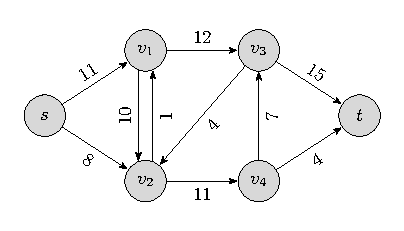
\includegraphics{network.pdf}
\end{center}

\begin{itemize}
    \item Systems of highways, railroads, shipping lanes, or aviation patterns, where some supply of a commodity is transported or distributed to satisfy a demand;
    \item pipeline systems or utility grids can be viewed as fluid flow or power flow networks;
    \item computer communication networks represent the flow of information;
    \item an economic system may represent the flow of wealth;
    \item routing a vehicle or a commodity between certain specified points in the network; 
    \item assigning jobs to machines, or matching workers with jobs for maximum efficiency; 
    \item project planning and project management, where various activities must be scheduled in order to minimize the duration of a project or to meet specified completion dates, subject to the availability of resources;
    \item and many, many others.
\end{itemize}

\section{Definitions}

    \begin{center}
    \scalebox{0.5}
    {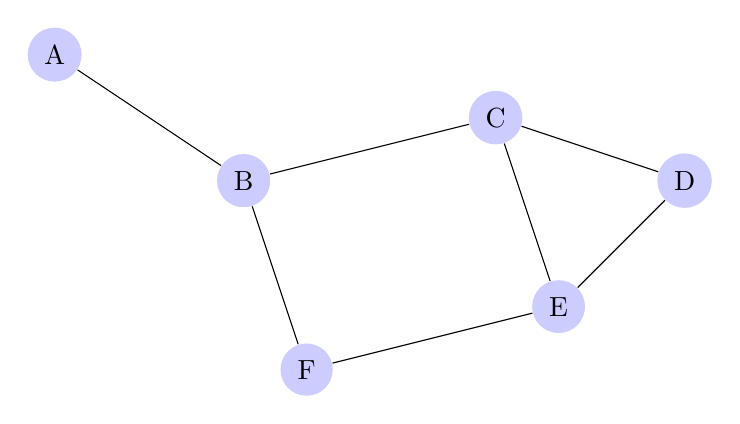
\begin{tikzpicture}
        [scale=.8,auto=left,every node/.style={circle,fill=blue!20}]
        \node (n6) at (1,10) {A};
        \node (n4) at (4,8)  {B};
        \node (n5) at (8,9)  {C};
        \node (n1) at (11,8) {D};
        \node (n2) at (9,6)  {E};
        \node (n3) at (5,5)  {F};    
        \foreach \from/\to in {n6/n4,n4/n5,n5/n1,n1/n2,n2/n5,n2/n3,n3/n4}
          \draw (\from) -- (\to);      
      \end{tikzpicture}
      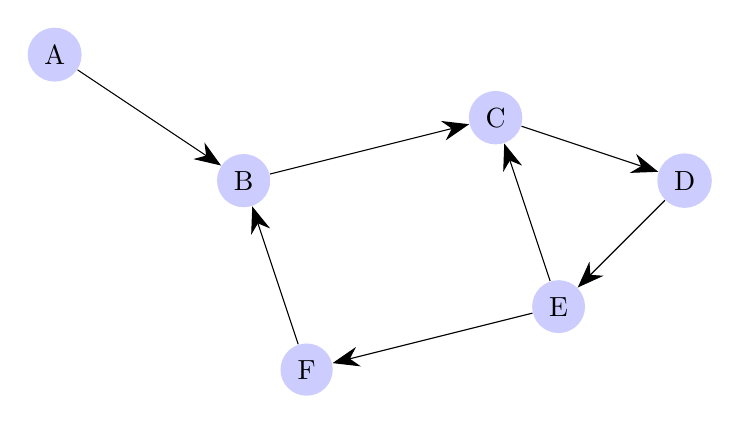
\begin{tikzpicture}
        [scale=.8,auto=left,every node/.style={circle,fill=blue!20}]
        \node (n6) at (1,10) {A};
        \node (n4) at (4,8)  {B};
        \node (n5) at (8,9)  {C};
        \node (n1) at (11,8) {D};
        \node (n2) at (9,6)  {E};
        \node (n3) at (5,5)  {F};    
        \foreach \from/\to in {n6/n4,n4/n5,n5/n1,n1/n2,n2/n5,n2/n3,n3/n4}
          \draw [-{Stealth[scale=2]}] (\from) -- (\to);      
      \end{tikzpicture}}
    \end{center}
\begin{itemize}
    \item A graph consists of a set of nodes $V$  (vertices, points, or junctions) and a set of connections called arcs $A$ (edges, links, or branches). 
    \item Each connection is associated with a pair of nodes and is usually drawn as a line joining two points. The graph can be defined as {\em directed} or {\em undirected}. 
    \item The {\bf degree of a node} is the number of arcs attached to it. An isolated node is of degree zero.
    \item In a directed graph, or digraph, the arc is often designated by the ordered pair $(A, B)$. In digraphs, the direction of the flow matters.
\end{itemize}

  \begin{center}
  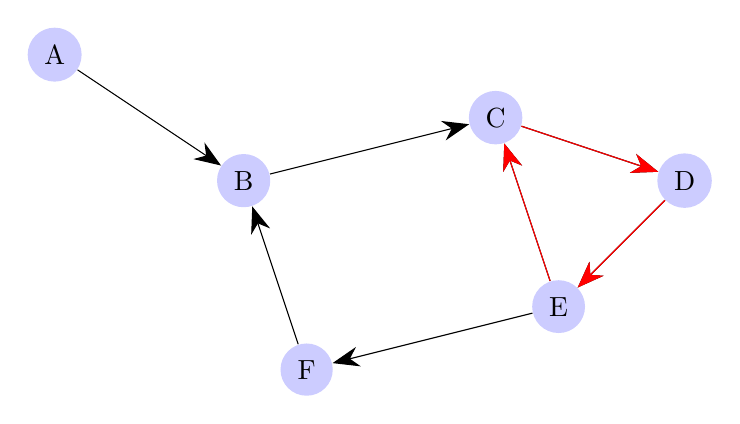
\begin{tikzpicture}
    [scale=.8,auto=left,every node/.style={circle,fill=blue!20}]
    \node (n6) at (1,10) {A};
    \node (n4) at (4,8)  {B};
    \node (n5) at (8,9)  {C};
    \node (n1) at (11,8) {D};
    \node (n2) at (9,6)  {E};
    \node (n3) at (5,5)  {F};    
    \foreach \from/\to in {n6/n4,n4/n5,n5/n1,n1/n2,n2/n5,n2/n3,n3/n4}
      \draw [-{Stealth[scale=2]}] (\from) -- (\to); 
    \foreach \from/\to in {n5/n1,n1/n2,n2/n5}
      \draw [red, -{Stealth[scale=2]}] (\from) -- (\to);     
  \end{tikzpicture}
\end{center}
\[A,(A,B),B,(B,C),\color{red}{\underbrace{C,(C,D),D,(D,E),E,(E,C),C}_{\mathrm{cyclic\, path \, and  \, chain}}}\]


  \begin{center}
  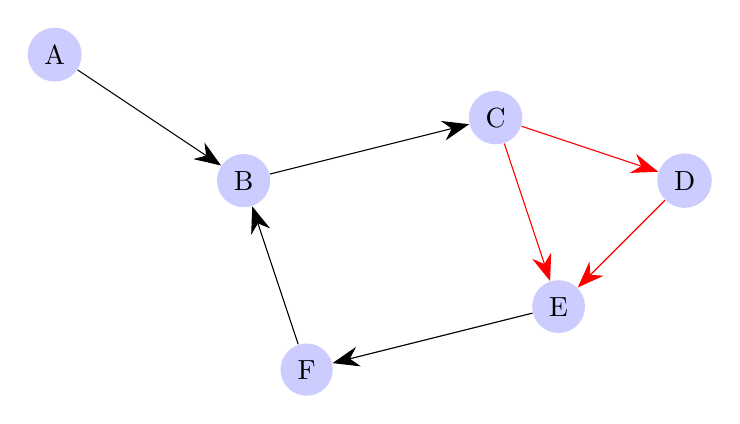
\begin{tikzpicture}
    [scale=.8,auto=left,every node/.style={circle,fill=blue!20}]
    \node (n6) at (1,10) {A};
    \node (n4) at (4,8)  {B};
    \node (n5) at (8,9)  {C};
    \node (n1) at (11,8) {D};
    \node (n2) at (9,6)  {E};
    \node (n3) at (5,5)  {F};    
    \foreach \from/\to in {n6/n4,n4/n5,n2/n3,n3/n4}
      \draw [-{Stealth[scale=2]}] (\from) -- (\to);      
    \foreach \from/\to in {n5/n1,n1/n2,n5/n2}
      \draw [red,-{Stealth[scale=2]}] (\from) -- (\to);      
  \end{tikzpicture}
\end{center}
\[A,(A,B),B,(B,C),\color{red}{\underbrace{C,(C,D),D,(D,E),E,(C,E),C}_{\mathrm{cyclic \, path, \,non \, cyclic  \, chain}}}\]


  \begin{itemize}
    \item If all the arcs in a path are forward arcs, the path is called {\bf directed chain} or simply {\bf chain}.
    \item {\bf path} and {\bf chain} are synonimous if the graph is undirected.
    \item In the second example above we saw a cyclic path but not a cyclic chain, as it included the backward arc $(C,E)$. 
    \item A {\bf connected graph} has at least one path connecting every pair of nodes.
    \item In a {\bf bipartite graph} the nodes can be partitioned into two subsets $S$ and $T$, such that each node is in exactly one of the subsets, and every arc in the graph connects a node in set $S$ with a node in set $T$.
    \item Such a graph is {\bf complete bipartite} if each node in $S$ is connected to every node in $T$.
  \end{itemize}

  \begin{center}
    \scalebox{0.7}
    {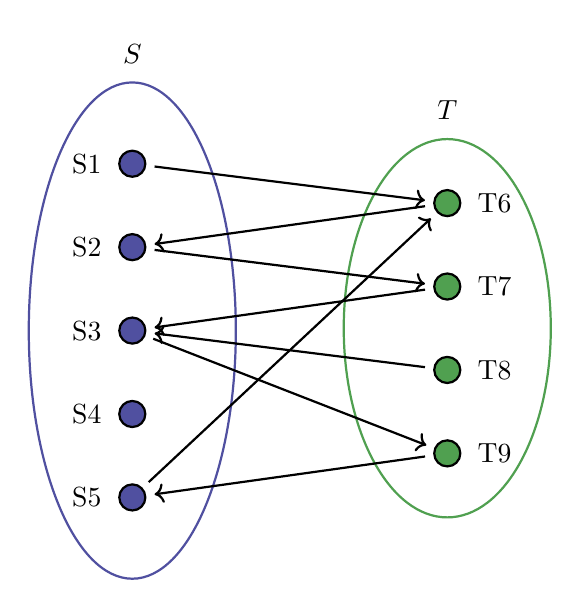
\begin{tikzpicture}[thick,
    every node/.style={draw,circle},
    fsnode/.style={fill=myblue},
    ssnode/.style={fill=mygreen},
    every fit/.style={ellipse,draw,inner sep=-2pt,text width=2cm},
    ->,shorten >= 3pt,shorten <= 3pt
  ]
  
  % the vertices of U
  \begin{scope}[start chain=going below,node distance=7mm]
  \foreach \i in {1,2,...,5}
    \node[fsnode,on chain] (f\i) [label=left: S\i] {};
  \end{scope}
  
  % the vertices of V
  \begin{scope}[xshift=4cm,yshift=-0.5cm,start chain=going below,node distance=7mm]
  \foreach \i in {6,7,...,9}
    \node[ssnode,on chain] (s\i) [label=right: T\i] {};
  \end{scope}
  
  % the set S
  \node [myblue,fit=(f1) (f5),label=above:$S$] {};
  % the set T
  \node [mygreen,fit=(s6) (s9),label=above:$T$] {};
  
  % the edges
  \draw (f1) -- (s6);
  \draw (s6) -- (f2);
  \draw (f2) -- (s7);
  \draw (s7) -- (f3);
  \draw (s8) -- (f3);
  \draw (f3) -- (s9);
  \draw (s9) -- (f5);
  \draw (f5) -- (s6);
  \end{tikzpicture}
  \hspace{3cm}
  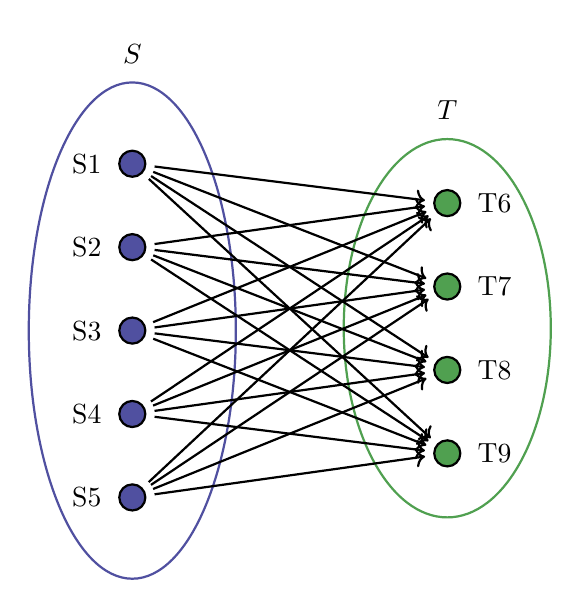
\begin{tikzpicture}[thick,
    every node/.style={draw,circle},
    fsnode/.style={fill=myblue},
    ssnode/.style={fill=mygreen},
    every fit/.style={ellipse,draw,inner sep=-2pt,text width=2cm},
    ->,shorten >= 3pt,shorten <= 3pt
  ]
  
  % the vertices of S
  \begin{scope}[start chain=going below,node distance=7mm]
  \foreach \i in {1,2,...,5}
    \node[fsnode,on chain] (f\i) [label=left: S\i] {};
  \end{scope}
  
  % the vertices of T
  \begin{scope}[xshift=4cm,yshift=-0.5cm,start chain=going below,node distance=7mm]
  \foreach \i in {6,7,...,9}
    \node[ssnode,on chain] (s\i) [label=right: T\i] {};
  \end{scope}
  
  % the set S
  \node [myblue,fit=(f1) (f5),label=above:$S$] {};
  % the set T
  \node [mygreen,fit=(s6) (s9),label=above:$T$] {};
  
  % the edges
  \draw (f1) -- (s6);
  \draw (f1) -- (s7);
  \draw (f1) -- (s8);
  \draw (f1) -- (s9);
  \draw (f2) -- (s6);
  \draw (f2) -- (s7);
  \draw (f2) -- (s8);
  \draw (f2) -- (s9);
  \draw (f3) -- (s6);
  \draw (f3) -- (s7);
  \draw (f3) -- (s8);
  \draw (f3) -- (s9);
  \draw (f4) -- (s6);
  \draw (f4) -- (s7);
  \draw (f4) -- (s8);
  \draw (f4) -- (s9);
  \draw (f5) -- (s6);
  \draw (f5) -- (s7);
  \draw (f5) -- (s8);
  \draw (f5) -- (s9);
  \end{tikzpicture}
  }
  \end{center}

  \begin{itemize}
    \item A {\bf tree} is a directed connected graph in which each node has at most on predecessor, and one node (the root node) has none. In an undirected graph, we have a tree if the graph is connected and contains no cycles.
    \begin{center}
    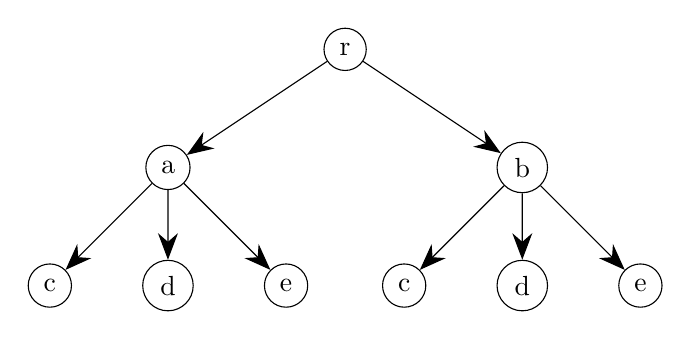
\begin{tikzpicture}[nodes={draw, circle}, -{Stealth[scale=2]}]
    \node{r}
    child { node {a} 
        child { node {c} }
        child { node {d} }
        child { node {e} }
    }
    child [missing]
    child [missing]
    child {node {b} 
        child { node {c} }
        child { node {d} }
        child { node {e} }
    };
  \end{tikzpicture}
\end{center}

    \item A {\bf network} is a directed connected graph that is used to model/represent a system/process. The arcs are typically assigned weights representing cost, value or capacity corresponding to each link.
    \item Nodes in networks can be designated as {\bf sources}, {\bf sinks} or {\bf transshipments}. A {\bf cut set} is any set of arcs which, if removed from the network, would disconnet the sources(s) from the sink(s).
    \item {\bf Flow} can be thought of as the total amount of an entity that originates at the source, makes it through the different nodes and reaches the sink.
  \end{itemize}

\section{Maximum flow}

  \begin{minipage}{7cm}{Maximum flow in networks}
    Determine the maximum possible flow that can be routed through the various network links, from source ($s$) to sink ($t$), without violating the capacity constraints.

    Important! the commodity is only generated at the source and consumed at the sink.
  \end{minipage}

  \begin{center}
    
  
  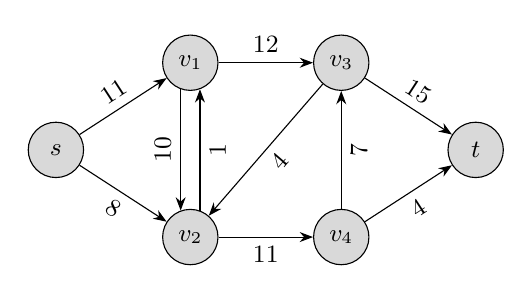
\begin{tikzpicture}[
    mycircle/.style={
       circle,
       draw=black,
       fill=gray,
       fill opacity = 0.3,
       text opacity=1,
       inner sep=0pt,
       minimum size=20pt,
       font=\small},
    myarrow/.style={-Stealth},
    node distance=0.6cm and 1.2cm
    ]
    \node[mycircle] (c1) {$s$};
    \node[mycircle,below right=of c1] (c2) {$v_2$};
    \node[mycircle,right=of c2] (c3) {$v_4$};
    \node[mycircle,above right=of c1] (c4) {$v_1$};
    \node[mycircle,right=of c4] (c5) {$v_3$};
    \node[mycircle,below right=of c5] (c6) {$t$};

  \foreach \i/\j/\txt/\p in {% start node/end node/text/position
    c1/c2/8/below,
    c1/c4/11/above,
    c2/c3/11/below,
    c3/c6/4/below,
    c4/c5/12/above,
    c5/c6/15/above,
    c5/c2/4/below,
    c3/c5/7/below,
    c2.70/c4.290/1/below}
     \draw [myarrow] (\i) -- node[sloped,font=\small,\p] {\txt} (\j);


   % draw this outside loop to get proper orientation of 10
   \draw [myarrow] (c4.250) -- node[sloped,font=\small,above,rotate=180] {10} (c2.110);
  \end{tikzpicture}
\end{center}
The {\bf maximum flow problem} can be stated as a LP formulation. 
\begin{equation*}
  \begin{aligned}
    \text{maximize } \quad & z = f \\
    \text{subject to }\quad &
    \begin{array}{rcl}
      \sum_{i=2}^n x_{1i}= f&& \\
      \sum_{i=1}^{n-1} x_{in} = f &&\\
      \sum_{i=1}^n x_{ij} = \sum_{k=1}^n x_{jk}, & \text{for } & j=2,3,\ldots,n-1\\
      x_{ij} \leq u_{ij}, & \text{for all } & i,j=1,2,\ldots,n
    \end{array}
  \end{aligned}
\end{equation*}
\note{Constraints (1) and (2) state that all the flow is generated at the source and consumed at the sink. Constraint (1) ensures that a flow of f leaves the source, and because of conservation of flow, that flow stops only at the sink. Constraints (3) are the flow conservation equations for all the intermediate nodes; nothing is generated or consumed at these nodes. Constraints (4) enforce arc capacity restrictions. All flow amounts xij must be non-negative. Actually, constraint (2) is redundant\cite{carter}}

  All network problems here can be solved using the Simplex method, but the network structure can help us solving it more efficiently. In the {\bf Ford-Fulkerson labelling algorithm}:
  \begin{enumerate}
    \item Use a labelling procedure to look for a flow augmenting path. If none can be found, stop; the current flow is optimal;
    \item Increase the current flow as much as possible in the flow augmenting path, until reaching capacity of some arc. Come back to step 1.
  \end{enumerate}

  \begin{Exercise}
    Find the maximum flow in this network using the Ford-Fulkerson labelling algorithm:
  \begin{center}
    
  
    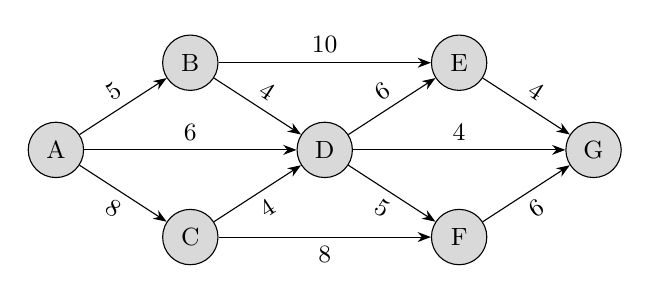
\begin{tikzpicture}[
      mycircle/.style={
         circle,
         draw=black,
         fill=gray,
         fill opacity = 0.3,
         text opacity=1,
         inner sep=0pt,
         minimum size=20pt,
         font=\small},
      myarrow/.style={-Stealth},
      node distance=0.6cm and 1.2cm
      ]
      \node[mycircle] (c1) {A};
      \node[mycircle,below right=of c1] (c2) {C};
      \node[mycircle,above right=of c1] (c3) {B};
      \node[mycircle,above right=of c2] (c4) {D};
      \node[mycircle,above right=of c4] (c5) {E};
      \node[mycircle,below right=of c4] (c6) {F};
      \node[mycircle,above right=of c6] (c7) {G};
  
    \foreach \i/\j/\txt/\p in {% start node/end node/text/position
      c1/c2/8/below,
      c1/c3/5/above,
      c1/c4/6/above,
      c3/c4/4/above,
      c2/c4/4/below,
      c3/c5/10/above,
      c2/c6/8/below,
      c4/c5/6/above,
      c4/c6/5/below,
      c4/c7/4/above,
      c5/c7/4/above,
      c6/c7/6/below}
       \draw [myarrow] (\i) -- node[sloped,font=\small,\p] {\txt} (\j);
    \end{tikzpicture}
  \end{center}
\end{Exercise}
\note{ Let us assume initially that the flow in all arcs is zero, x ij = 0 and f = 0. In the
first iteration, we label nodes A, B, C, D, and G, and discover the flow augmenting path (A,
D) and (D, G), across which we can increase the flow by 4. So now, x AD = 4, xDG = 4, and f = 4.
In the second iteration, we label nodes A, B, C, then nodes E, D, and F, and finally node G.
A flow augmenting path consists of links (A, B), (B, D), (D, E), and (E, G) and flow on this
path can be increased by 4. Now x AB = 4, xBD = 4, xDE = 4, x EG = 4, and f = 8.
In the third iteration, we see that there remains some unused capacity on link (A, B), so
we can label nodes A, B, and E, but not G. It appears we cannot use the full capacity of link
(A, B). However, we can also label nodes C, D, F, and G, and augment the flow along the
links (A, D), (D, F), and (F, G) by 2, the amount of remaining capacity in (A, D). Now x AD = 6,
xDF = 2, x FG = 2, and f = 10.
In the fourth iteration, we can label nodes A, B, C, D, F, and G. Along the path from A,
C, D, F, to G, we can add a flow of 4, the remaining capacity in (F, G). So x AC = 4, xCF = 4,
x FG = 6, and f = 14.
In the fifth iteration, we can label all nodes except G. Therefore, there is no flow aug-
menting path, and the current flow of 14 is optimal\cite{carter}}

  \begin{itemize}
    \item In any network, there is always a bottleneck that in some sense impedes the flow through the network. 
    \item The total capacity of the bottleneck is an upper bound on the total flow in the network. 
    \item Cut sets are, by definition, essential in order for there to be a flow from source to sink, since removal of the cut set links would render the sink unreachable from the source. 
    \item The capacities on the links in any cut set potentially limit the total flow. 
    \item The minimum cut (i.e., the cut set with minimum total capacity) is in fact the bottleneck that precisely determines the maximum possible flow in the network (Max-Flow Min-Cut Theorem): the capacity of the cut is precisely equal to the current flow and this flow is optimal. In other words, a saturated cut defines the maximum flow.
  \end{itemize}

  We can generate a supersource or  a  supersink node with unlimited capacity and repeat the process of optimization as above:\cite{carter}
  \begin{center}
    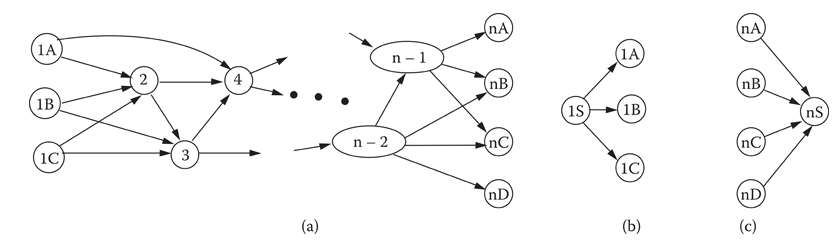
\includegraphics[width=\linewidth]{multiplesinkssources.png}
  \end{center}

\section{Minimum Cost Network Flow}

\begin{itemize}
  \item Useful when there are costs associated with the flow, given a link capacity. 
  \item Let us assume that every node is a source (supply) and a sink (demand). Imagine a distributor with several warehouses and a group of costumers. Serving each customer from a given warehouse has an associated cost.
  \item For $m$ supply nodes, each providing $s_i$ suplly,  and $n$ demand nodes, each demanding $d_j$. Assuming that the total demand eaquals the total supply: $\sum_{i=1}^m s_i = \sum_{j=1}^n d_j$ we aim at satisfying the demand using the available supply minimizing cost routes.
\end{itemize}

  \begin{equation*}
    \begin{aligned}
      \text{minimize } \quad & z = \sum_{i=1}^m \sum_{j=1}^n c_{ij}x_{ij} \\
      \text{subject to }\quad &
      \begin{array}{rcl}
        \sum_{j=1}^n x_{ij}= s_i&\text{for }& i=1,\ldots,m \\
        \sum_{i=1}^m x_{ij} = d_j &\text{for }& j=1,\ldots,n \\
        x_{ij} \geq 0 & \text{for all } & i,j
      \end{array}
    \end{aligned}
  \end{equation*}
  \begin{center}
    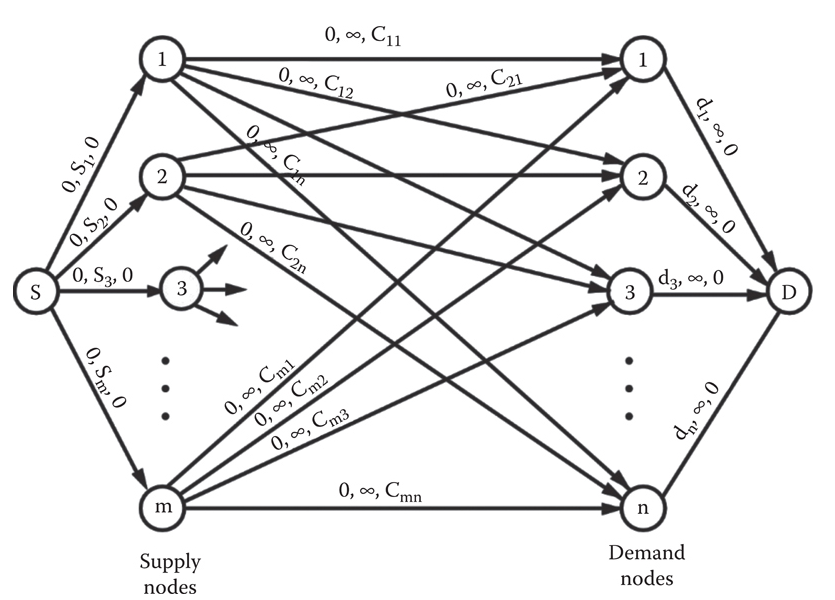
\includegraphics[width=0.55\linewidth]{transportationproblem.png}
  \end{center}

\begin{Exercise}
  Find the minimum cost in this trasportation problem:\cite{carter}
  \begin{center}
    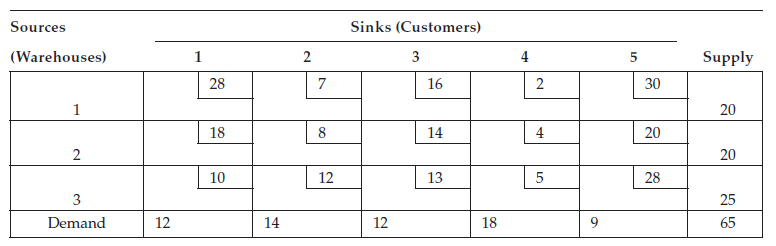
\includegraphics[width=\linewidth]{transportationproblem2.png}
  \end{center}
  NOTE: The Simplex method says that we should first find any basic feasible solution and then look for a simple pivot to improve the solution. repeat until the optimal solution is found.
\end{Exercise}

\begin{enumerate}
  \item Finding initial solution.
  \begin{itemize}
  \item Northwest corner rule
  \item Minimum cost method
  \item Minimum "row" cost method
  \item Vogel's method (opportunity cost)
  \end{itemize}
  \item Transportation simplex
\end{enumerate}

  Once we have any feasible solution, we aim at finding the optimal one. Consider:
  \begin{center}
    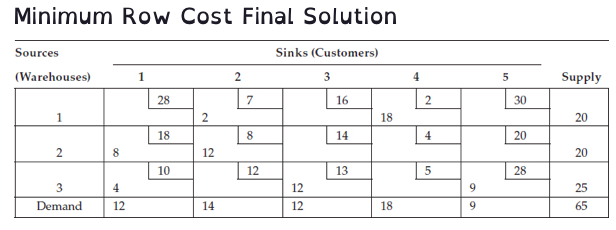
\includegraphics[width=\linewidth]{transportationproblem3.png}
  \end{center}


  We can reduce the total cost by reducing the individual costs in every row $i$ by $u_i$ and in every column $j$ by $v_j$:
  \[c'_{ij}=c_{ij}-u_i-v_j\]
  Check that, now:
  \begin{itemize}
    \item $\sum_i \sum_j x_{ij} c'_{ij}=0$
    \item Check how some costs are now negative in non-basic cells. 
    \item If we increase the number of units in those non-basic cells from 0 to some value, reducing at the same time the number of units in the basic cells, we can reduce the overall cost $\sum_i \sum_j x_{ij} c_{ij}$
  \end{itemize} 


In practice:
\begin{enumerate}
  \item We find first an initial feasible solution as explained above
  \item Calculate the $u_i$ and $v_j$, taking into account that $c_{ij}=u_i+v_j$, for all basic variables (used squares in the table). We start by assigning $u_1=0$.
  \item We calculate the {\em improvement index} by $I_{ij}=c_{ij}-u_i-v_j$ for all non-used squares in the table.
  \item If all $I_{ij}$ are positive, the solution is already optimal and we are done.
  \item If some $I_{ij}<0$, then build a loop with such value in the corner and alternative $\pm$ signs in all vertex. 
  \item Use the above $\pm$ to increase the number of units in the position that had $I_{ij}<0$
  \item We return to step 2.
\end{enumerate}

%   \resizebox*{\textwidth}{!}{ 
%   \begin{tabular}{c|C|C|C|C|C|r}\hline
%     & 1 & 2 & 3 & 4 & 5 & Supply  \\\hline
% 1   & \innerbox{}{28} & \innerbox{2}{7} & \innerbox{}{16} & \innerbox{18}{2} & \innerbox{}{30} &   20   \\\hline
% 2   & \innerbox{8}{18} & \innerbox{12}{8} & \innerbox{}{14}  & \innerbox{}{4} & \innerbox{}{20}  &   20   \\\hline
% 3   & \innerbox{4}{10} & \innerbox{}{12} & \innerbox{12}{13} & \innerbox{}{5} & \innerbox{9}{28}   &  25   \\\hline
% Demand & \bottombox{12} & \bottombox{14} & \bottombox{12} & \bottombox{18} & \bottombox{9} & 65   \\\hline
% \end{tabular}}

\note{dynamic programming: https://www.youtube.com/watch?v=jqyfhFziDjw

https://www.techiedelight.com/word-break-problem/

}
%----------------------------------------------------------------------------------------


%%%%%%%%%%%%%%%%%%%%%%%%%%%%%%%%%%%%%%%%%
% Beamer Presentation
% LaTeX Template
% Version 1.0 (10/11/12)
%
% This template has been downloaded from:
% http://www.LaTeXTemplates.com
%
% License:
% CC BY-NC-SA 3.0 (http://creativecommons.org/licenses/by-nc-sa/3.0/)
%
%%%%%%%%%%%%%%%%%%%%%%%%%%%%%%%%%%%%%%%%%

%----------------------------------------------------------------------------------------
%	PACKAGES AND THEMES
%----------------------------------------------------------------------------------------

\documentclass[c]{beamer}
%\documentclass[notes]{beamer}
\input{../OR_common.tex}

\usepackage{array}
\newcolumntype{C}{@{}c@{}}
\newcommand{\bottombox}[1]{\makebox[2em][r]{#1}\hspace*{\tabcolsep}\hspace*{2em}}%
\newcommand{\innerbox}[2]{%
    \begin{tabular}[b]{c|c}
       \rule{2em}{0pt}\rule[-2ex]{0pt}{5ex} & \makebox[2em]{#2} \\\cline{2-2}
       \multicolumn{2}{r}{{#1}\hspace*{1.5\tabcolsep}\hspace*{2em}\rule[-2ex]{0pt}{5ex}}
    \end{tabular}}
\renewcommand{\arraystretch}{1.25}

%%%%%%%%%%%%%%%%%%%%%%%%%%%%%%%%%%%%%%%%%%%%%%%%%%%%%%%%%%%%%%%%%%%%%%%%%%%%%
%%%%%%%%%%%%%%%%%%%%%%%%%%%%%%%%%%%%%%%%%%%%%%%%%%%%%%%%%%%%%%%%%%%%%%%%%%%%%
%%%%%%%%%%%%%%%%%%%%%%%%%%%%%%%%%%%%%%%%%%%%%%%%%%%%%%%%%%%%%%%%%%%%%%%%%%%%%

\title[Introduction]{Unit 4. Integer Programming}


%%%%%%%%%%%%%%%%%%%%%%%%%%%%%%%%%%%%%%%%%%%%%%%%%%%%%%%%%%%%%%%%%%%%%%%%%%%%%
%%%%%%%%%%%%%%%%%%%%%%%%%%%%%%%%%%%%%%%%%%%%%%%%%%%%%%%%%%%%%%%%%%%%%%%%%%%%%
%%%%%%%%%%%%%%%%%%%%%%%%%%%%%%%%%%%%%%%%%%%%%%%%%%%%%%%%%%%%%%%%%%%%%%%%%%%%%

\begin{itemize}
  \item Getting familiar with the use of integer programming
  \item Solving integer programming problems
\end{itemize}

\begin{itemize}
  \item Problems in which the feasible set is composed of only integer values.
  \item The feasible set is neither continuous nor feasible.
  \item NP-hard problems in general.
  \item Integer problems that have a network structure are easy to solve using the Simplex method (assignment and matching problems, transportation and transshipment problems, and network flow problems always produce integer results, provided that the problem bounds are integers).
  \item Rounding can be effective in some problems and clearly not in others:
  \begin{itemize}
    \item not the same tires than aircrafts!
    \item values 0/1 for variable: zero-one or binary integer programming (produce or not produce cars in this factory)
    \item mixed integer programming problems
  \end{itemize} 
\end{itemize}


  \begin{equation*}
    \begin{aligned}
      \text{maximize } \quad & \sum_{j=1}^{n} c_j x_j \\
      \text{subject to }\quad &
      \begin{array}{rcl}
        \sum_{j=1}^n a_{ij} x_j= b_i&i=1,2,\ldots,m&  \\
        x_j > 0 &j=1,2,\ldots,n&\\
        x_j \quad \mathrm{integer} & \mathrm{for\,some\,or\,all\,} & j=1,2,\ldots,n
      \end{array}
    \end{aligned}
  \end{equation*}



    \begin{center}
      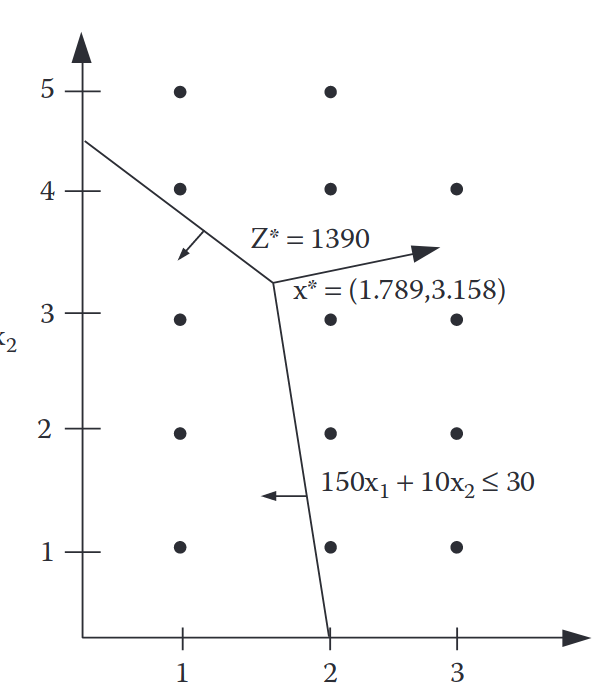
\includegraphics[width=0.4\linewidth]{../figures/IntegerProgramming.png}
    \end{center}
    Graphical representation of a typical 2 dimensional integer programming\cite{carter}.


  
    \begin{itemize}
      \item Capital budgeting: deciding between a collection of investiments
      \item Warehouse location: in modelling distribution systems, we should decide about tradeoffs between transportation costs and costs for operating distributions centers
      \item Scheduling: students-faculty-classrooms allocations, vehicle dispatching, etc (see next slide)
    \end{itemize}
  


  {\bf Airline crew scheduling problem}: The airlines first design a flight schedule composed of a large number of {\em flight legs} (specific flight on a specific piece of equipment, such as a 747 from New York to Chicago departing at 6:27 a.m.). A flight crew is a complete set of people, including pilots, navigator, and flight attendants who are trained for a specific airplane. A work schedule or rotation is a collection of flight legs that are feasible for a flight crew, and that normally terminate at the point of origin. Variables $x_{ij}$ have value 1 if flight leg $i$ is assigned to crew $j$. All flight legs should be covered at minimum total cost. 
  \\[10pt]
  Also called a {\em set-partitioning problem}
  \begin{equation*}
    \begin{aligned}
      \text{minimize } \quad & \sum_{j=1}^{n} c_j x_j \\
      \text{subject to }\quad &
      \begin{array}{rcl}
        \sum_{j=1}^n a_{ij} x_j= 1&i=1,2,\ldots,m&  \\
        x_j = {0,1} &j=1,2,\ldots,n
      \end{array}
    \end{aligned}
  \end{equation*}



  \begin{Exercise}
    Consider the travelling salesman problem. Starting from his home, a salesman wishes to visit each of $(n-1)$ other cities and return home at minimal cost. He must visit each city exactly once and the cost to travel from city $i$ to $j$ is $c_{ij}$. Let $x_{ij}$ be 1 or 0 depending on the fact that he goes or not from city $i$ to city $j$
    \begin{itemize}
      \item formulate the optimization problem
      \item how to avoid disjoint tours?
    \end{itemize}
  \end{Exercise}



  Simplex is not useful to solve, in general, integer problems. Instead, many other techniques have been proposed:
  \begin{itemize}
    \item Enumeration techniques, including the branch-and-bound procedure;
    \item cutting plane techniques; and 
    \item group-theoretic techniques,
  \end{itemize}

  as well as several composite techniques
  




    \begin{center}
      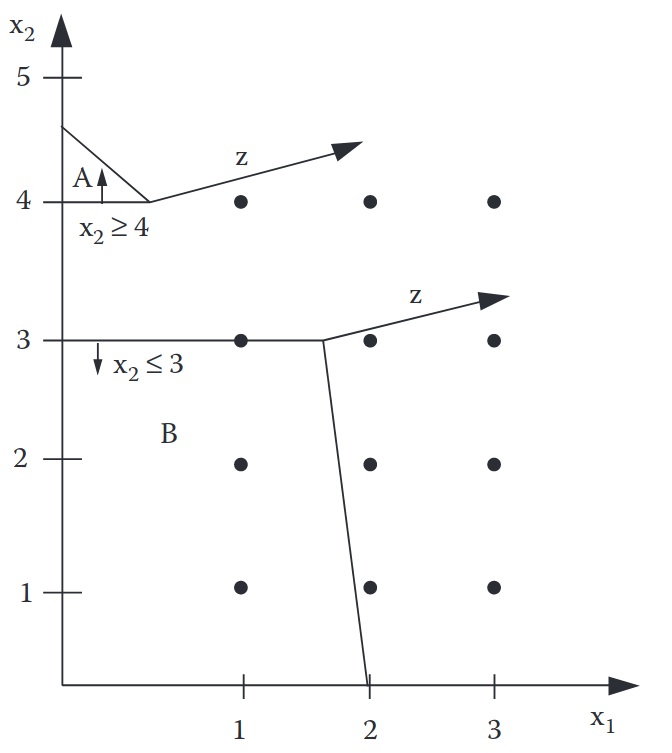
\includegraphics[width=0.4\linewidth]{../figures/BranchandBound.png}
    \end{center}
    Separation into two subproblems in the Branch-and-Bound method\cite{carter}.


  \begin{Exercise}
    Using the graphical representation and the branch-and-bound procedure, solve this integer program:
    \begin{equation*}
      \begin{aligned}
        \text{maximize } \quad & z=x_1+5x_2 \\
        \text{subject to }\quad &
        \begin{array}{rcl}
          -4x_1+3x_2\leq 6&&  \\
          3x_1+2x_2\leq 18&&  \\
          x_1,x_2 \geq 0 & \mathrm{and\,integer}
        \end{array}
      \end{aligned}
    \end{equation*}
  \end{Exercise}





\section{References}

%----------------------------------------------------------------------------------------


%%%%%%%%%%%%%%%%%%%%%%%%%%%%%%%%%%%%%%%%%
% Beamer Presentation
% LaTeX Template
% Version 1.0 (10/11/12)
%
% This template has been downloaded from:
% http://www.LaTeXTemplates.com
%
% License:
% CC BY-NC-SA 3.0 (http://creativecommons.org/licenses/by-nc-sa/3.0/)
%
%%%%%%%%%%%%%%%%%%%%%%%%%%%%%%%%%%%%%%%%%

%----------------------------------------------------------------------------------------
%	PACKAGES AND THEMES
%----------------------------------------------------------------------------------------

\documentclass[c]{beamer}
%\documentclass[notes]{beamer}
\input{../OR_common.tex}

% \usepackage{array}
% \newcolumntype{C}{@{}c@{}}
% \newcommand{\bottombox}[1]{\makebox[2em][r]{#1}\hspace*{\tabcolsep}\hspace*{2em}}%
% \newcommand{\innerbox}[2]{%
%     \begin{tabular}[b]{c|c}
%        \rule{2em}{0pt}\rule[-2ex]{0pt}{5ex} & \makebox[2em]{#2} \\\cline{2-2}
%        \multicolumn{2}{r}{{#1}\hspace*{1.5\tabcolsep}\hspace*{2em}\rule[-2ex]{0pt}{5ex}}
%     \end{tabular}}
% \renewcommand{\arraystretch}{1.25}

%%%%%%%%%%%%%%%%%%%%%%%%%%%%%%%%%%%%%%%%%%%%%%%%%%%%%%%%%%%%%%%%%%%%%%%%%%%%%
%%%%%%%%%%%%%%%%%%%%%%%%%%%%%%%%%%%%%%%%%%%%%%%%%%%%%%%%%%%%%%%%%%%%%%%%%%%%%
%%%%%%%%%%%%%%%%%%%%%%%%%%%%%%%%%%%%%%%%%%%%%%%%%%%%%%%%%%%%%%%%%%%%%%%%%%%%%

\title[Introduction]{Unit 5. Stochastic processes}



%%%%%%%%%%%%%%%%%%%%%%%%%%%%%%%%%%%%%%%%%%%%%%%%%%%%%%%%%%%%%%%%%%%%%%%%%%%%
%%%%%%%%%%%%%%%%%%%%%%%%%%%%%%%%%%%%%%%%%%%%%%%%%%%%%%%%%%%%%%%%%%%%%%%%%%%%%
%%%%%%%%%%%%%%%%%%%%%%%%%%%%%%%%%%%%%%%%%%%%%%%%%%%%%%%%%%%%%%%%%%%%%%%%%%%%%

\section{Markov chains}

\begin{Exercise}
    Here is a simple game:
\begin{itemize}
    \item a player bets on coin tosses, a dollar each time,
    \item the game ends either when the player has no money left
    or is up to five dollars.
\end{itemize}
If the player starts with three dollars, what is the chance that the game
    takes at least five flips?
    Twenty-five flips?
\end{Exercise}

At any point, this player has either \$0, or \$1, \ldots, or \$5.
We say that the player is in the
state
$s_0$, $s_1$, \ldots, or $s_5$.
A game consists of moving from state to state.
For instance,
a player now in state $s_3$ has on the next flip a $.5$ chance of moving
to state $s_2$ and a $.5$ chance of moving to $s_4$.
The boundary states are a bit different;
once in state~$s_0$ or state~$s_5$,
the player never leaves.



Let $p_{i}(n)$ be the probability that the player is in state $s_i$
after $n$ flips.
Then, for instance, we have that the probability of being in state~$s_0$
after flip~$n+1$ is
$p_{0}(n+1)=p_{0}(n)+0.5\cdot p_{1}(n)$.
This matrix equation sumarizes.
\begin{equation*}
  \begin{pmatrix}
      1  &.5 &0  &0  &0   &0  \\
      0  &0  &.5 &0  &0   &0  \\
      0  &.5 &0  &.5 &0   &0  \\
      0  &0  &.5 &0  &.5  &0  \\
      0  &0  &0  &.5 &0   &0  \\
      0  &0  &0  &0  &.5  &1
   \end{pmatrix}
   \colvec{p_{0}(n) \\
        p_{1}(n) \\
        p_{2}(n) \\
        p_{3}(n) \\
        p_{4}(n) \\
        p_{5}(n)}
   =\colvec{p_{0}(n+1) \\
        p_{1}(n+1) \\
        p_{2}(n+1) \\
        p_{3}(n+1) \\
        p_{4}(n+1) \\
        p_{5}(n+1)}
\end{equation*}

With the initial condition that the player starts with
three dollars, calculation gives this.
\begin{center}
  \begin{tabular}{@{}c|cccccc@{}}
    $n=0$
    &$n=1$
    &$n=2$
    &$n=3$
    &$n=4$
    &$\cdots$
    &$n=24$ \\
    \hline
    $\left(\begin{aligncolondecimal}{0}
             0 \\ 0    \\  0   \\  1    \\  0    \\  0
           \end{aligncolondecimal}
     \right)$
    &$\left(\begin{aligncolondecimal}{1}
       0      \\  0    \\  .5  \\  0    \\  .5    \\  0
             \end{aligncolondecimal}
     \right)$
    &$\left(\begin{aligncolondecimal}{2}
      0      \\  .25  \\ 0    \\ .5    \\  0     \\  .25
            \end{aligncolondecimal}
     \right)$
    &$\left(\begin{aligncolondecimal}{3}
        .125   \\   0   \\ .375 \\ 0     \\ .25    \\  .25
            \end{aligncolondecimal}
     \right)$
    &$\left(\begin{aligncolondecimal}{4}
        .125   \\ .1875 \\ 0    \\ .3125 \\ 0      \\ .375
            \end{aligncolondecimal}
     \right)$
    &$\cdots$
    &$\left(\begin{aligncolondecimal}{5}
        .39600 \\ .00276   \\ 0    \\ .00447 \\ 0  \\ .59676
            \end{aligncolondecimal}
     \right)$
  \end{tabular}
\end{center}

\begin{itemize}
    \item The player quickly ends in either state~$s_0$
    or state~$s_5$. For instance, after the fourth flip there is a probability of $0.50$ that
    the game is already over: The boundary states
    are said to be {\bf absorbtive}.
    \item {\em The Markov chain model is
    historyless}: with a fixed transition matrix, the next state depends only on the current state,
    not on any prior states. More formally:
    \begin{eqnarray*}
    P(x_{t+1}=s_{t+1}|x_t=s_t, x_{t-1}=s_{t-1},...,x_1=s_1,x_0=s_0)=\\
    P(x_{t+1}=s_{t+1}|x_t=s_t)
  \end{eqnarray*}
    \item In addition, it is clear that the probability of a transition from state $i$ to state $j$ is independent of time ({\bf stationarity property}):
    \[
    P(x_{t+1}=j|x_t=i)=p_{ij}
    \]
    \item Each column vector is a probability vector (and it sums up 1) and the matrix is a transition matrix.
\end{itemize}


\begin{Exercise}
    A study (\cite{MacdonaldRidge}, p.~202)
divided occupations in the United Kingdom into
upper level (executives and professionals),
middle level (supervisors and skilled manual workers),
and lower level (unskilled).
To determine
the mobility across these levels in a generation, about
two thousand men were asked, ``At which level are you,
and at which level was your father when you were fourteen years old?''
\end{Exercise}

This equation and transition diagram summarizes the results.

  \begin{center}
\begin{equation*}
  \begin{pmatrix}
    T_{1,1}  &T_{1,2}  &T_{1,3}  \\
    T_{2,1}  &T_{2,2}  &T_{2,3}  \\
    T_{3,1}  &T_{3,2}  &T_{3,3}
  \end{pmatrix}^t
\rightarrow
    \begin{pmatrix}
      .60  &.29  &.16  \\
      .26  &.37  &.27  \\
      .14  &.34  &.57
    \end{pmatrix}
    \colvec{p_{U}(n) \\ p_{M}(n) \\ p_{L}(n)}
    =\colvec{p_{U}(n+1) \\ p_{M}(n+1) \\ p_{L}(n+1)}
  \end{equation*}
    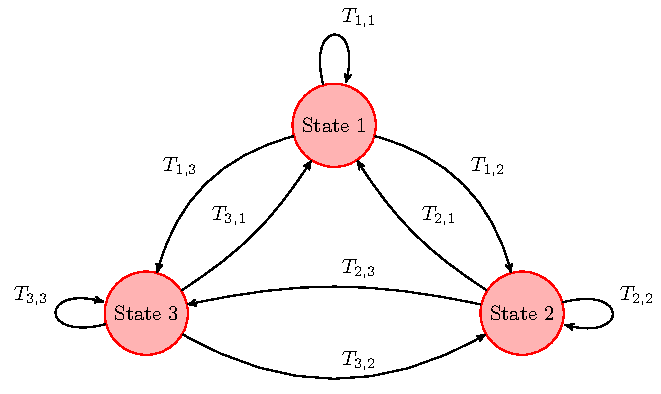
\includegraphics[width=0.7\linewidth]{../figures/transitiondiagram.pdf}
  \end{center}

For instance,
a child of a lower class worker has a $.27$ probability of
growing up to be middle class.
Notice that the Markov model assumption about history
seems reasonable-- we expect that
while a parent's occupation has a direct influence on the occupation of the
child, the grandparent's occupation has no such direct influence.
With the initial distribution of the respondents's fathers given below,
this table lists the
distributions for the next five generations.
\begin{center}
  \begin{tabular}{c|ccccc}
    $n=0$  &$n=1$  &$n=2$  &$n=3$  &$n=4$  &$n=5$  \\ \hline
     $\left(\begin{aligncolondecimal}{2} .12 \\ .32  \\ .56 \end{aligncolondecimal} \right)$
    &$\left(\begin{aligncolondecimal}{2} .23 \\ .34  \\ .42 \end{aligncolondecimal} \right)$
    &$\left(\begin{aligncolondecimal}{2} .29 \\ .34  \\ .37 \end{aligncolondecimal} \right)$
    &$\left(\begin{aligncolondecimal}{2} .31 \\ .34  \\ .35 \end{aligncolondecimal} \right)$
    &$\left(\begin{aligncolondecimal}{2} .32 \\ .33  \\ .34 \end{aligncolondecimal} \right)$
    &$\left(\begin{aligncolondecimal}{2} .33 \\ .33  \\ .34 \end{aligncolondecimal} \right)$
  \end{tabular}
\end{center}

\begin{Exercise}
The World Series of American baseball is
played between the team winning the American League
and the team winning the National League.
The series is won by the first team to win four games.
That means that a series is in one of twenty-four states:
0-0 (no games won yet by either team), 1-0
(one game won for the American League
team and no games for the National League team), etc.
If we assume that there is a probability $p$ that
the American League team wins each game then we have the following transition
matrix.
\end{Exercise}

\begin{equation*}
  \begin{pmatrix}
    0      &0      &0      &0   &\ldots  \\
    p      &0      &0      &0   &\ldots  \\
    1-p    &0      &0      &0   &\ldots  \\
    0      &p      &0      &0   &\ldots  \\
    0      &1-p    &p      &0   &\ldots  \\
    0      &0      &1-p    &0   &\ldots  \\
    \vdots &\vdots &\vdots &\vdots
  \end{pmatrix}
  \colvec{p_{\text{0-0}}(n) \\ p_{\text{1-0}}(n) \\ p_{\text{0-1}}(n) \\
           p_{\text{2-0}}(n) \\ p_{\text{1-1}}(n) \\ p_{\text{0-2}}(n) \\
  \vdots }
  =
  \colvec{p_{\text{0-0}}(n+1) \\ p_{\text{1-0}}(n+1) \\ p_{\text{0-1}}(n+1) \\
           p_{\text{2-0}}(n+1) \\ p_{\text{1-1}}(n+1) \\ p_{\text{0-2}}(n+1) \\
           \vdots }
\end{equation*}
An especially interesting special case is $p=0.50$; this table lists the
resulting components of the $n=0$ through $n=7$ vectors. Check what happens with other values of $p$.


\begin{center}\small
    \resizebox*{!}{0.8\textheight}{
\begin{tabular}{@{}rl|lllllll@{}}
      &$n=0$  &$n=1$  &$n=2$  &$n=3$  &$n=4$  &$n=5$  &$n=6$  &$n=7$  \\ \hline
  $\begin{array}{@{}c@{}}
    0-0 \\
    1-0 \\
    0-1 \\
    2-0 \\
    1-1 \\
    0-2 \\
    3-0 \\
    2-1 \\
    1-2 \\
    0-3 \\
    4-0 \\
    3-1 \\
    2-2 \\
    1-3 \\
    0-4 \\
    4-1 \\
    3-2 \\
    2-3 \\
    1-4 \\
    4-2 \\
    3-3 \\
    2-4 \\
    4-3 \\
    3-4
  \end{array}$
  &$\begin{aligncolondecimal}{0}
     1 \\
     0 \\
     0 \\
     0 \\
     0 \\
     0 \\
     0 \\
     0 \\
     0 \\
     0 \\
     0 \\
     0 \\
     0 \\
     0 \\
     0 \\
     0 \\
     0 \\
     0 \\
     0 \\
     0 \\
     0 \\
     0 \\
     0 \\
     0
   \end{aligncolondecimal}$
  &$\begin{aligncolondecimal}{1}
        0           \\
        0.5         \\
        0.5         \\
        0           \\
        0           \\
        0           \\
        0           \\
        0           \\
        0           \\
        0           \\
        0           \\
        0           \\
        0           \\
        0           \\
        0           \\
        0           \\
        0           \\
        0           \\
        0           \\
        0           \\
        0           \\
        0           \\
        0           \\
        0
   \end{aligncolondecimal}$
  &$\begin{aligncolondecimal}{2}
        0           \\
        0           \\
        0           \\
        0.25        \\
        0.5         \\
        0.25        \\
        0           \\
        0           \\
        0           \\
        0           \\
        0           \\
        0           \\
        0           \\
        0           \\
        0           \\
        0           \\
        0           \\
        0           \\
        0           \\
        0           \\
        0           \\
        0           \\
        0           \\
        0
   \end{aligncolondecimal}$
  &$\begin{aligncolondecimal}{3}
        0            \\
        0            \\
        0            \\
        0            \\
        0            \\
        0            \\
        0.125        \\
        0.375        \\
        0.375        \\
        0.125        \\
        0            \\
        0            \\
        0            \\
        0            \\
        0            \\
        0            \\
        0            \\
        0            \\
        0            \\
        0            \\
        0            \\
        0            \\
        0            \\
        0
   \end{aligncolondecimal}$
  &$\begin{aligncolondecimal}{4}
        0              \\
        0              \\
        0              \\
        0              \\
        0              \\
        0              \\
        0              \\
        0              \\
        0              \\
        0              \\
        0.0625         \\
        0.25           \\
        0.375          \\
        0.25           \\
        0.0625         \\
        0              \\
        0              \\
        0              \\
        0              \\
        0              \\
        0              \\
        0              \\
        0              \\
        0
   \end{aligncolondecimal}$
  &$\begin{aligncolondecimal}{4}
        0              \\
        0              \\
        0              \\
        0              \\
        0              \\
        0              \\
        0              \\
        0              \\
        0              \\
        0              \\
        0.0625         \\
        0              \\
        0              \\
        0              \\
        0.0625         \\
        0.125          \\
        0.3125         \\
        0.3125         \\
        0.125          \\
        0              \\
        0              \\
        0              \\
        0              \\
        0
   \end{aligncolondecimal}$
  &$\begin{aligncolondecimal}{5}
        0               \\
        0               \\
        0               \\
        0               \\
        0               \\
        0               \\
        0               \\
        0               \\
        0               \\
        0               \\
        0.0625          \\
        0               \\
        0               \\
        0               \\
        0.0625          \\
        0.125           \\
        0               \\
        0               \\
        0.125           \\
        0.15625         \\
        0.3125          \\
        0.15625         \\
        0               \\
        0
   \end{aligncolondecimal}$
  &$\begin{aligncolondecimal}{5}
        0             \\
        0             \\
        0             \\
        0             \\
        0             \\
        0             \\
        0             \\
        0             \\
        0             \\
        0             \\
        0.0625        \\
        0             \\
        0             \\
        0             \\
        0.0625        \\
        0.125         \\
        0             \\
        0             \\
        0.125         \\
        0.15625       \\
        0             \\
        0.15625       \\
        0.15625       \\
        0.15625
   \end{aligncolondecimal}$
\end{tabular}}
\end{center}

Evenly-matched teams are likely to have a long series-- there
is a probability of $0.625$ that the series goes at least six games.

  In summary, a system can be modeled as a Markov process if it has the following four properties:
  \begin{itemize}
    \item Property 1: A finite number of states can be used to describe the dynamic behavior of the system.
    \item Property 2: Initial probabilities are specified for the system.
    \item Property 3: Markov property—We assume that a transition to a new state depends only on the current state and not on past conditions.
    \item Property 4: Stationarity property—The probability of a transition between any two states does not vary in time.
  \end{itemize}


  If  Markov analysis is appropriate for the system being studiedone can try answering questions like:
\begin{itemize}
  \item How many transitions (steps) will it likely take for the system to move from some specified state to another specified state?
  \item What is the probability that it will take some given number of steps to go from one specified state to another?
  \item In the long run, which state is occupied by the system most frequently?
  \item Over a long period of time, what fraction of the time does the system occupy each of the possible states?
  \item Will the system continue indefinitely to move among all $N$ states, or will it eventually settle into a certain few states?
\end{itemize}

\note{dynamic programming: https://www.youtube.com/watch?v=jqyfhFziDjw

https://www.techiedelight.com/word-break-problem/
}

\section{Hidden Markov Models}


  HMMs are probably the most popular directed graphical model out there. They are used in many sequential and temporal domains:
  \begin{itemize}
    \item speech recognition,
    \item handwriting recognition,
    \item visual target tracking and localization,
    \item machine translation,
    \item robot localization,
    \item gene prediction,
    \item time-series analysis,
    \item natural language processing and part-of-speech recognition,
    \item stochastic control,
    \item protein folding, ...
  \end{itemize}

  In HMMs, the random variables are divided into hidden states (phonemes, letters, target location) and observations (audio signal, pen strokes, target image). The goal is to predict the states from observations.

  What is this?
\begin{center}
  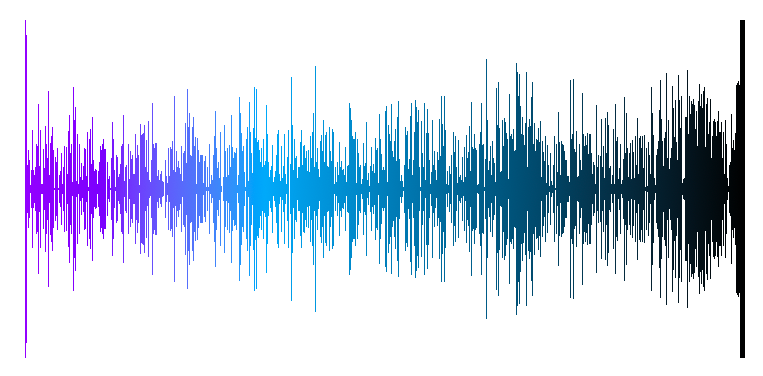
\includegraphics[width=0.7\linewidth]{../figures/SultansofSwing.png}
\end{center}

We can start wth the graphical representation of the HMM
\begin{center}
 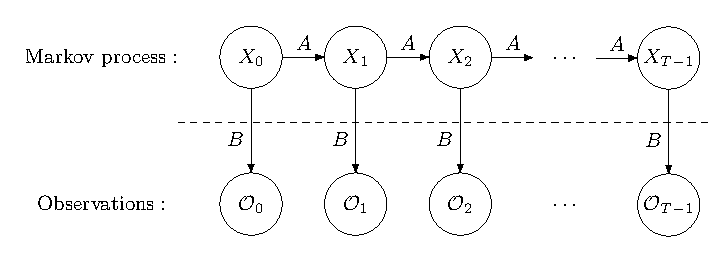
\includegraphics[width=0.7\linewidth]{../figures/HMM.pdf}
\end{center}

% To learn more on HMM:
% \begin{itemize}
%   \item \url{https://alliance.seas.upenn.edu/~cis520/wiki/index.php?n=Lectures.HMMs#toc7}
%   \item \url{http://www.columbia.edu/~mh2078/MachineLearningORFE/HMMs_MasterSlides.pdf}
% \end{itemize}

\section{Discrete Evenet Simulations (DES)}
  \begin{center}
    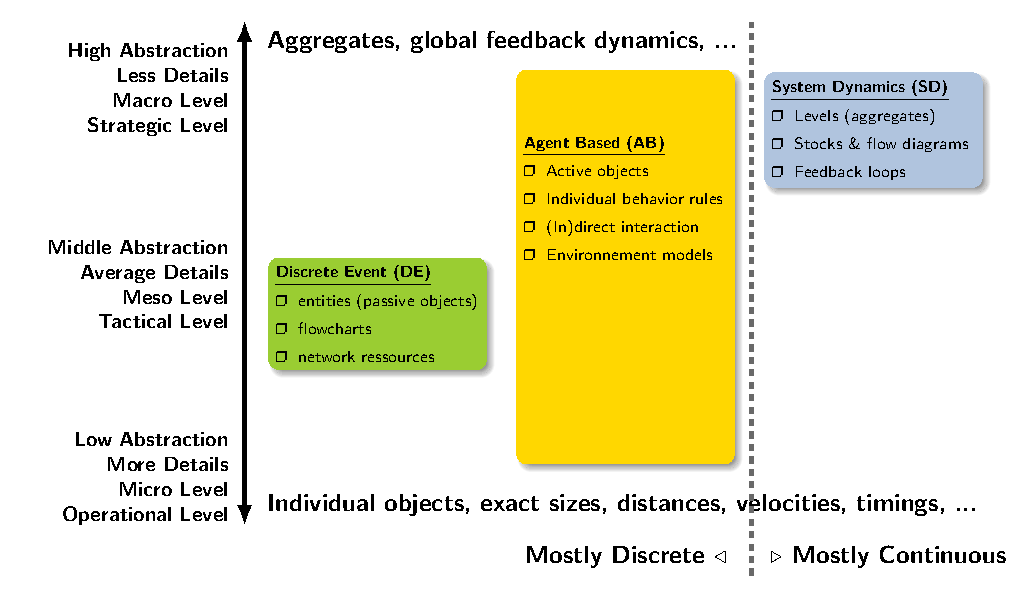
\includegraphics[width=0.7\linewidth]{../figures/simulation.pdf}
  \end{center}
  Taken from \url{https://texample.net/tikz/examples/simulation-abstraction/}

%----------------------------------------------------------------------------------------

\end{document}
